% ----------- Cover Master Thesis Faculty of Sciences ---------------
% This document should be compiled with pdflatex.  If you want to use
% latex to compile to dvi/ps, you have to convert the images to (e)ps
%                           -- December 2012
% -------------------------------------------------------------------
\RequirePackage{fix-cm}
\documentclass[12pt,a4paper,oneside]{book}

% ------------------------- Load packages ---------------------------
% You can eventually add these while you load other packages
% in case you want to integrate the titlepage with the rest of your thesis
% -------------------------------------------------------------------
\usepackage{graphicx,xcolor,textpos}


\renewcommand{\familydefault}{\sfdefault} % one could turn off this one
\usepackage{helvet}                       % one could turn off this one
%\usepackage[scaled=0.92]{helvet}
%\usepackage[scaled=1]{newtxsf}
\usepackage[helvet]{sfmath}               % one could turn off this one
%\usepackage{cmbright}
\usepackage{amsmath, amsfonts, amssymb}
\usepackage{booktabs}
%\usepackage[style = chem-acs]{biblatex}
\usepackage[numbers,sort&compress]{natbib}
\usepackage{siunitx}
\usepackage{subcaption}
\usepackage{svg}
\usepackage[T1]{fontenc}
\usepackage{setspace}
\usepackage{hyperref}
%\usepackage[nottoc,numbib]{tocbibind}
\usepackage{algorithm}
\usepackage{algpseudocode}

% ------------------------ Page settings -----------------------------
% If you change these, the cover layout will also change.  In that
% case you have to adjust the latter manually.
% --------------------------------------------------------------------

\topmargin -10mm
\textwidth 160truemm
\textheight 240truemm
\oddsidemargin 0mm
\evensidemargin 0mm

% ---------------------- textpos settings ----------------------------
% Some additional settings for the cover
% --------------------------------------------------------------------

\definecolor{green}{RGB}{172,196,0}
\definecolor{bluetitle}{RGB}{29,141,176}
\definecolor{blueaff}{RGB}{0,0,128}
\definecolor{blueline}{RGB}{82,189,236}
\setlength{\TPHorizModule}{1mm}
\setlength{\TPVertModule}{1mm}

\begin{document}

% ----------------------- Cover --------------------------------------
% Please fill in:
% - The title and subtitle (if applicable)
%         to include a formula in the title or subtitle
%         use  \form{$...$}
% - Your name
% - Your (co)supervisor, mentor (if applicable)
% - Your master
% - The academic year
% --------------------------------------------------------------------
\thispagestyle{empty}
\newcommand{\form}[1]{\scalebox{1.087}{\boldmath{#1}}}
\sffamily % one could change this one to 'rmfamily'
%
\begin{textblock}{191}(-24,-11)
\colorbox{bluetitle}{\hspace{139mm}\ \parbox[c][18truemm]{52mm}{\textcolor{white}{FACULTY OF SCIENCE}}}
\end{textblock}
%
\begin{textblock}{70}(-18,-19)
\textblockcolour{}
\includegraphics*[height=19.8truemm]{LogoKULeuven}
\end{textblock}
%
\begin{textblock}{160}(-6,63)
\textblockcolour{}
\vspace{-\parskip}
\flushleft
\fontsize{35}{37}\selectfont \textcolor{bluetitle}{\textit{Ab Initio} Molecular Dynamics Simulations of Phosphate Hydrolysis Using Neural Network Potentials}\\[1.5mm]
%\fontsize{20}{22}\selectfont Dynamics and Reactivity
\end{textblock}
%
\begin{textblock}{160}(8,153)
\textblockcolour{}
\vspace{-\parskip}
\flushright
\fontsize{14}{16}\selectfont \textbf{Albert MAKHMUDOV}
\end{textblock}
%
\begin{textblock}{70}(-6,191)
\textblockcolour{}
\vspace{-\parskip}
\flushleft
Supervisor: Prof. J. Harvey\\[-2pt]
\textcolor{blueaff}{KU Leuven}\\[5pt]
%Mentor: Prof. J. Harvey\\[-2pt]
%\textcolor{blueaff}{KU Leuven}\\
\end{textblock}
%
\begin{textblock}{160}(8,191)
\textblockcolour{}
\vspace{-\parskip}
\flushright
Thesis presented in\\[4.5pt]
fulfillment of the requirements\\[4.5pt]
for the degree of Master of Science\\[4.5pt]
in Theoretical Chemistry and Computational Modelling\\
\end{textblock}
%
\begin{textblock}{160}(8,232)
\textblockcolour{}
\vspace{-\parskip}
\flushright
Academic year 2024-2025
\end{textblock}
%
\begin{textblock}{191}(-24,248)
{\color{blueline}\rule{550pt}{5.5pt}}
\end{textblock}
%


% In case you want to integrate the TeX-file for the titlepage
% with the rest of your thesis, you cab continue below
% ------------------------- First pages ---------------------------
% For table of contents, acknowlegments, ...
% -----------------------------------------------------------------
%\rmfamily
\setcounter{page}{0}
\pagenumbering{roman}
\onehalfspacing

\mbox{}
\thispagestyle{empty}
\vfill
\noindent \textbf{© Copyright by KU Leuven}
\par\bigskip
\noindent Without written permission of the promotors and the authors it is forbidden to reproduce or adapt in any form or by
any means any part of this publication. Requests for obtaining the right to reproduce or utilize parts of this publication should be addressed to KU Leuven, Faculteit Wetenschappen, Celestijnenlaan 200H bus 2100, 3001 Leuven
(Heverlee), telephone +32 16 32 14 01.
\par\bigskip
\noindent A written permission of the promotor is also required to use the methods, products, schematics and programs
described in this work for industrial or commercial use, and for submitting this publication in scientific contests.
\par\bigskip
\noindent This thesis is an exam document that obtained no further correction of possible errors after the defense. Referring to this thesis in papers and analogous documents is only allowed after written consent of the supervisor(s), mentioned on the title page.
\chapter*{Foreword}  

The TCCM master's programme - and this thesis project in particular - provided me with the opportunity to open a completely new chapter of my life. Not only did it allow me to study at a top-notch university, but, more importantly, it gave me the chance to be surrounded by brilliant people who inspired me to think outside the box and to learn many new things, not merely in a professional sense, but also on a personal level.

\par\smallskip
I'm wholeheartedly grateful to my supervisor, Prof. Jeremy Harvey, who agreed to take me on from the time of my internship in the first year and continued to support me throughout the master's thesis. His constant guidance and encouragement made this project possible. However, most significantly, our discussions and brainstorming sessions had the greatest impact on me. They helped me to think critically about my research topic and to consider it from different perspectives.

\par\smallskip
I'd like to thank my family in Uzbekistan for always being there for me and supporting me within the course of my studies. Their love and support helped me get through all the ups and downs of living in a completely new environment. \begin{otherlanguage}{russian} Большое спасибо моей семье: маме, бабушке, папе и младшему брату за веру в меня. Люблю вас всех и крепко обнимаю! Без вашей поддержки у меня бы точно не получилось начать новую жизнь в совершенно другой части мира. \end{otherlanguage}

\par\smallskip
Student life is not only about studying, but also about making friends and having fun. In this regard, I would like to thank those I hold dear: my friends, all group and division members, as well as the TCCM cohort, for making these two years an unforgettable experience. Special \textit{dank u wel}, \textit{muchas gracias}, \textit{merci beaucoup}, and \textit{muito obrigado} go to everyone for the coffee breaks we shared - they were not only a great way to unwind, but also a source of eureka moments and ideas.

\par\smallskip
Last but not least, I would like to express my gratitude to my former supervisors and colleagues in Uzbekistan, who motivated me to embark on an academic journey and to pursue a master's degree abroad. For that, I would like to thank Dr. Artyom Baev, Dr. Anvar Sariev, Prof. Zukhra Kadirova, and Prof. Shahlo Daminova. 

\par\smallskip
This project would not have been possible without the computational resources provided by KU Leuven and the Erasmus+ scholarship from the EMJMD TCCM.


\chapter*{Contribution statement}
Albert Makhmudov proposed revisiting phosphate hydrolysis using a more advanced computational setup. Prof. Jeremy Harvey suggested the investigation of a system containing methyl diphosphate and proposed the use of a neural network potential to describe the reaction mechanism. The overall workflow was designed together by Albert Makhmudov and Prof. Jeremy Harvey, who also jointly analysed the results. All calculations, figures, and visualisations were carried out by Albert Makhmudov. The thesis was written by Albert Makhmudov with feedback and corrections from Prof. Jeremy Harvey. Ehsan Moravveji (VSC, KU Leuven), Hans Vansweevelt (KU Leuven), and Anders Johansson (Harvard) helped with the installation and compilation of the software on the high-performance computing clusters.
\chapter*{Summary}
Stearoyl-CoA desaturase (SCD1) plays an important role in the metabolism of fatty acids and is a promising therapeutic target. However, the underlying mechanism of SCD1, as well as other transmembrane non-heme diiron enzymes, remains poorly understood. This study builds upon a previous DFT cluster model study which proposed a potential reactive intermediate of SCD1. We assessed its dynamical properties by employing classical and multiscale molecular dynamics (MD) simulations. Our classical MD simulations revealed that the proposed intermediate lacks the ability to form a favourable reactive complex with stearoyl-CoA, highlighting the significance of a conserved asparagine residue in controlling the substrate's orientation. Motivated by these observations, we proposed a new intermediate in which a water molecule is strategically placed to stabilize the conserved asparagine residue. Subsequent classical MD simulations showed that the new intermediate is able to form a reactive complex with the substrate, consistent with the experimentally observed selectivity of SCD1. The free energy barrier for the first hydrogen atom abstraction (HAA) step on C$_{9}$ by the new intermediate was estimated to be 16.9 kcal/mol. The estimate is based on a hybrid quantum mechanics/molecular mechanics (QM/MM) approach utilizing the efficient semiempirical GFN2-xTB method in combination with B3LYP energy corrections. Considering its computational efficiency, GFN2-xTB seems to be a promising tool for the study of complex transition metal systems. Overall, our findings provide valuable insights into the mechanism of SCD1, thereby advancing the understanding of the entire class of transmembrane non-heme diiron enzymes. Furthermore, the findings can potentially help in the design of new inhibitors.

%\chapter*{Summary accessible to the broad public}
%Enzymes are important proteins that accelerate chemical reactions in our bodies. They typically achieve this by reducing the energy required for a reaction to occur. However, in many cases, we do not fully understand the details of how enzymes accomplish this. Experimental studies can be very challenging, so it is common to employ computer simulations to help us understand how enzymes work. Computer simulations try to mimic the atomic behaviour of the real system using some approximate models based on classical and/or quantum mechanics. The enzyme of interest in this thesis is stearoyl-CoA desaturase (SCD1). It plays a crucial role in the metabolism of fatty acids and has been linked to increased cancer growth. Studies found that its inhibition can slow down cancer growth, making it a promising therapeutic target. This thesis builds upon a previous study which suggested a potential reactive intermediate involved in the reactivity of SCD1. We used advanced computer simulations to investigate the proposed intermediate in more detail. The simulations showed that the proposed intermediate lacked the ability to interact favourably with its target molecule. Based on these results, we proposed a new intermediate that should better stabilize the rest of the protein structure and make it more favourable. Subsequent simulations indeed showed that the new intermediate is able to combine with its target molecule in a manner consistent with experimental observations. Additionally, we estimated the energy needed for the reaction to occur and found that it falls in the range typical for other enzymes, further supporting our proposal. Our findings advance the understanding of SCD1 and related enzymes, potentially helping in the design of new drugs targeting SCD1.
\chapter*{List of abbreviations}

\begin{table}[htbp]
    \begin{tabular}{ll}
%   SCD1 & Stearoyl-CoA desaturase \\
    \end{tabular}
\end{table}



\tableofcontents



\newpage
% -------------------------- Proper text --------------------------
% Introduction, chapters, ...
% -----------------------------------------------------------------
\setcounter{page}{0}
\pagenumbering{arabic}

\chapter{Introduction}
This chapter provides an overview of the role of phosphates in biological systems, the enzymes involved in phosphate hydrolysis, and a detailed explanation of the reaction mechanisms associated with these processes - topics that have puzzled researchers for a long time. The discussion begins with the fundamental importance of phosphates in life, particularly in energy transfer and storage. This is followed by a brief overview of the enzymes that catalyse phosphate hydrolysis and their implications for cellular function. Finally, the chapter explores the reaction mechanisms of phosphate hydrolysis, highlighting key studies and findings in this area.

\section{Role of phosphates in biological systems}
Phosphates are among the fundamental building blocks that play a central role in life on Earth. They form the basis for both the storage and transfer of genetic information, as well as the flow of metabolic energy within biological systems. The ubiquitous nature of phosphate esters and anhydrides - such as those found in \ac{dna}, \ac{rna}, \ac{atp}, and \ac{polyp} - highlights their fundamental importance \citep{westheimerWhyNatureChose1987}. Some of the phosphates found in biological systems and their respective functions are summarised in Table~\ref{tab:role_of_phosphates}.

A key characteristic enabling these roles is the ability of phosphoric acid to link molecular units while retaining an ionisable group. This inherent negative charge at physiological pH serves a dual purpose: it helps to retain these molecules within cellular boundaries defined by lipid membranes, and more importantly, it confers kinetic stability upon phosphate esters and anhydrides by electrostatically repelling nucleophilic attack, particularly from water \citep{westheimerWhyNatureChose1987}. For instance, the half-time for hydrolysis at 25\textdegree{C} for a pyrophosphate dianion is about 280 days; however, for a pyrophosphate trianion, this number increases dramatically to 10 years \citep{wolfendenDegreesDifficultyWaterConsuming2006}. This stability is crucial for maintaining the integrity of genetic material but can be readily overcome by enzymatic catalysis when there is a metabolic demand.

Phosphates are involved in numerous processes in living systems, such as cell signalling and sensation, regulation of metabolism, blood coagulation, and bone formation \citep{mullerInorganicPolyphosphatesStorage2019, nebesnayaInorganicPolyphosphateRegulates2024}. Their role is perhaps most evident in cellular energetics, where \ac{atp} functions as the universal energy currency. The energy derived from nutrients such as glucose is captured and stored within the high-energy phosphoanhydride bonds linking the phosphate groups of \ac{atp}. This energy is released upon hydrolysis of the terminal phosphoanhydride bond (P-O bond between $\beta$ and $\gamma$ in Figure~\ref{fig:atp}), typically yielding \ac{adp} and \ac{Pi}. The cleavage of this bond provides the thermodynamic driving force for the majority of cellular processes, including biosynthesis, active transport, and mechanical work such as muscle contraction. The standard free energy change for ATP hydrolysis is substantial ($\Delta G^{0}=-30.5$ kJ mol$^{-1}$), and under cellular conditions, the actual free energy release is often considerably greater. Specifically, the experimentally obtained $\Delta G$ values are approximately $-59$ to $-53.5$ kJ mol$^{-1}$ in the liver and about $-61.7$ to $-59.5$ kJ mol$^{-1}$ in the heart \citep{mullerInorganicPolyphosphatesStorage2019}.

\begin{table}[b!]
    \centering
    \begin{tabular}{cc}
    \toprule
    \textbf{Phosphate} & \textbf{Biological role} \\ 
    \midrule
    DNA/RNA & Genetic material \\
    ADP/ATP & Intracellular energy transfer \\
    cAMP & Cellular signalling \\
    Polyphosphate & Energy storage, Cellular signalling \\
    Creatine phosphate & Intracellular energy transfer \\
    Phosphoenolpyruvate & Metabolism \\
    Pyridoxal phosphate & Coenzyme \\
    Nicotine adenine dinucleotide & Calcium signalling \\
    Fructose 1,6-diphosphate & Metabolism \\
    Glucose-6-phosphate & Metabolism \\
    Isopentenyl pyrophosphate & Metabolism \\
    Ribose-6-phosphate & Metabolism \\
    Glycerol 3-phosphate & Metabolism \\
    Dihydroxyacetone phosphate & Calvin cycle, metabolism \\
    Inositol phosphates & Cellular signalling \\
    \bottomrule
    \end{tabular}
    \caption{Examples of biologically relevant phosphates and their roles. Reproduced and adapted from~\citep{kamerlinWhyNatureReally2013}.}
    \label{tab:role_of_phosphates}
\end{table}

Beyond \ac{atp}, \ac{polyp} - a linear polymer of orthophosphate residues linked by similar high-energy phosphoanhydride bonds - represents another significant phosphate-based energy storage found across all domains of life, including mammalian cells. However, in mammalian cells, the concentration of \ac{polyp} is significantly lower compared to that in microorganisms. While its roles in mammals are still being fully elucidated, \ac{polyp} metabolism is intrinsically linked to the cellular energy status. Mitochondrial \ac{polyp} levels fluctuate with respiratory activity and appear to depend on F\textsubscript{0}F\textsubscript{1}-ATP synthase function, suggesting a role in mitochondrial bioenergetics, potentially acting as an energy reservoir \citep{pavlovInorganicPolyphosphateEnergy2010}.

The efficient transfer of energy stored in phosphate bonds from sites of production (e.g., mitochondria) to sites of utilisation (e.g., ATPases involved in muscle contraction or ion transport) is crucial. Simple diffusion of \ac{atp} is often insufficient due to the complexity of intracellular architecture and the potential for large concentration gradients to arise, which would be thermodynamically inefficient. Instead, cells employ phosphotransfer networks, utilising enzymes such as creatine kinase and adenylate kinase, which catalyse phosphoryl exchange reactions. These networks act as 'phosphoryl wires', facilitating the efficient conduction of high-energy phosphoryl groups and energetic signals throughout the cell with minimal energy dissipation or accumulation of inhibitory products such as \ac{adp}. The existence of these networks underscores the dynamic and highly organised nature of cellular energy management, where phosphates - mainly in the form of \ac{atp} - serve as the key energy carriers \citep{dzejaPhosphotransferNetworksCellular2003}.

The synthesis of \ac{atp} occurs primarily through oxidative phosphorylation in mitochondria, a process tightly coupled to the electron transport chain, which establishes a proton-motive force ($\Delta p$) across the inner mitochondrial membrane. This electrochemical potential energy is used by the molecular machine ATP synthase. Interestingly, the principal energy input required by ATP synthase is not for the chemical formation of the phosphoanhydride bond itself, but rather for the conformational changes necessary to release the newly synthesised, tightly bound \ac{atp} molecule from the enzyme's catalytic site. This 'binding change mechanism' involves the cooperative, sequential action of the enzyme's multiple catalytic sites, driven by proton flow. The hydrolysis of \ac{atp} to \ac{adp} and \ac{Pi} is catalysed by a variety of enzymes, including ATPases and possibly F\textsubscript{1}-ATPase, which are frequently coupled to other cellular processes \citep{boyerEnergyLifeATP1998}.

In summary, the unique chemical properties of phosphates - their ability to form stable esters and energy-rich anhydrides, along with their negative charge - combined with the evolution of sophisticated enzymatic machinery for their synthesis, transfer, and hydrolysis, have secured their vital role in virtually all life processes.



\section{Enzymes involved in phosphate hydrolysis}
The hydrolysis of high-energy phosphoanhydride bonds, particularly the terminal bond in \ac{atp}, is a cornerstone of cellular bioenergetics. While numerous enzymes utilise \ac{atp} hydrolysis, the F\textsubscript{0}F\textsubscript{1}-ATP synthase complex, primarily known for synthesising \ac{atp}, also shows potential \ac{atp} hydrolytic activity, particularly through its F\textsubscript{1} component (F\textsubscript{1}-ATPase). This enzyme complex, therefore, plays a dual role in managing the cell's primary energy currency \citep{bonoraATPSynthesisStorage2012, boyerEnergyLifeATP1998, walkerATPSynthaseUnderstood2013}. Furthermore, recent evidence suggests that this complex may also participate in the metabolism, including the hydrolysis, of \ac{polyp} in mammalian cells \citep{baevInorganicPolyphosphateF0F1ATP2022, baevInorganicPolyphosphateProduced2020}.

The F\textsubscript{0}F\textsubscript{1}-ATP synthase is a molecular motor embedded in the mitochondrial membrane. It consists of two major domains: the F\textsubscript{1} domain, which carries the catalytic sites, and the F\textsubscript{0} domain, which is embedded within the membrane. These domains are connected by a central rotor stalk and a peripheral stator stalk \citep{walkerATPSynthesisRotary1998, walkerATPSynthaseUnderstood2013, wattBioenergeticCostMaking2010}. The activity of this enzyme is coupled with the electron-transport chain, as illustrated in Figure~\ref{fig:atp_synthase}.

\begin{figure}[t!]
    \centering
    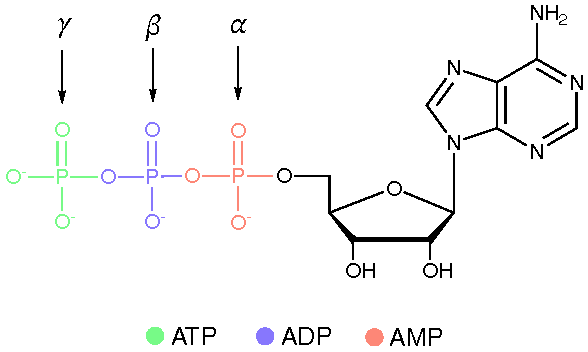
\includegraphics[width=0.6\textwidth]{Figures/1_Introduction/intro_atp.pdf}
    \caption{Chemical structures of the AMP, ADP, and ATP molecules with the phosphates marked as $\alpha$, $\beta$, and $\gamma$, respectively.}
    \label{fig:atp}
\end{figure}

The F\textsubscript{1} domain ($\alpha_3\beta_3\gamma\delta\epsilon$ stoichiometry) extends into the mitochondrial matrix. It has a globular shape as can be seen in Figure~\ref{fig:atp_synthase}. The catalytic sites for \ac{atp} synthesis and hydrolysis are located on the three $\beta$ subunits, which interact with the $\alpha$ subunits. When functioning in reverse, the F\textsubscript{1} domain acts as an F\textsubscript{1}-ATPase, hydrolysing \ac{atp}. This hydrolysis drives the counterclockwise rotation (as viewed from the membrane) of the central stalk, composed of the $\gamma$, $\delta$, and $\epsilon$ subunits \citep{walkerATPSynthesisRotary1998, walkerATPSynthaseUnderstood2013, boyerEnergyLifeATP1998}. If coupled to the F\textsubscript{0} domain, this rotation actively pumps protons from the matrix, thereby generating or maintaining the proton-motive force ($\Delta p$). This reverse function is especially important under conditions of low $\Delta p$, where it helps to prevent the complete dissipation of the proton-motive force at the expense of cellular \ac{atp} and possibly \ac{polyp} \citep{bonoraATPSynthesisStorage2012, walkerATPSynthaseUnderstood2013, baevInorganicPolyphosphateProduced2020}.

The mechanism of \ac{atp} hydrolysis (cleavage of the P-O bond between $\beta$ and $\gamma$ in Figure~\ref{fig:atp}) follows the principles of the binding change mechanism \citep{walkerATPSynthaseUnderstood2013}. The rotation of the asymmetric $\gamma$ subunit induces sequential conformational changes in the three $\beta$ subunits, cycling them through states analogous to those in synthesis: an 'open' state that binds \ac{atp}, a 'tight' state that facilitates hydrolysis, and a subsequent 'open' state that releases \ac{adp} and \ac{Pi} \citep{walkerATPSynthesisRotary1998, boyerEnergyLifeATP1998}. The hydrolysis of each \ac{atp} molecule is associated with a 120\textdegree{} rotation of the central stalk, which occurs in substeps \citep{walkerATPSynthaseUnderstood2013}.

While the metabolism of inorganic \ac{polyp} is well-characterised in microorganisms via specific kinases (PPK) and phosphatases (PPX), the enzymes responsible for its turnover in mammalian cells remain largely unknown. Recent studies using immunocaptured F\textsubscript{0}F\textsubscript{1}-ATPase have demonstrated that the enzyme complex can hydrolyse \ac{polyp}. This \ac{polyp} hydrolysis appears to drive the enzyme's proton-pumping activity, akin to \ac{atp} hydrolysis, and is sensitive to oligomycin, a specific F\textsubscript{0}F\textsubscript{1}-ATP synthase inhibitor. Medium- and long-chain \ac{polyp} molecules, made of 60 and 130 orthophosphate units, respectively, seem to be effective substrates for this hydrolytic activity. Docking simulations support the feasibility of \ac{polyp} binding to the nucleotide-binding sites within the F\textsubscript{1} domain. This suggests that \ac{polyp} could serve as an alternative energy source for the F\textsubscript{0}F\textsubscript{1} complex, potentially helping to maintain mitochondrial membrane potential when \ac{atp} levels are compromised \citep{baevInorganicPolyphosphateProduced2020, baevInorganicPolyphosphateF0F1ATP2022}.

\begin{figure}[t!]
    \centering
    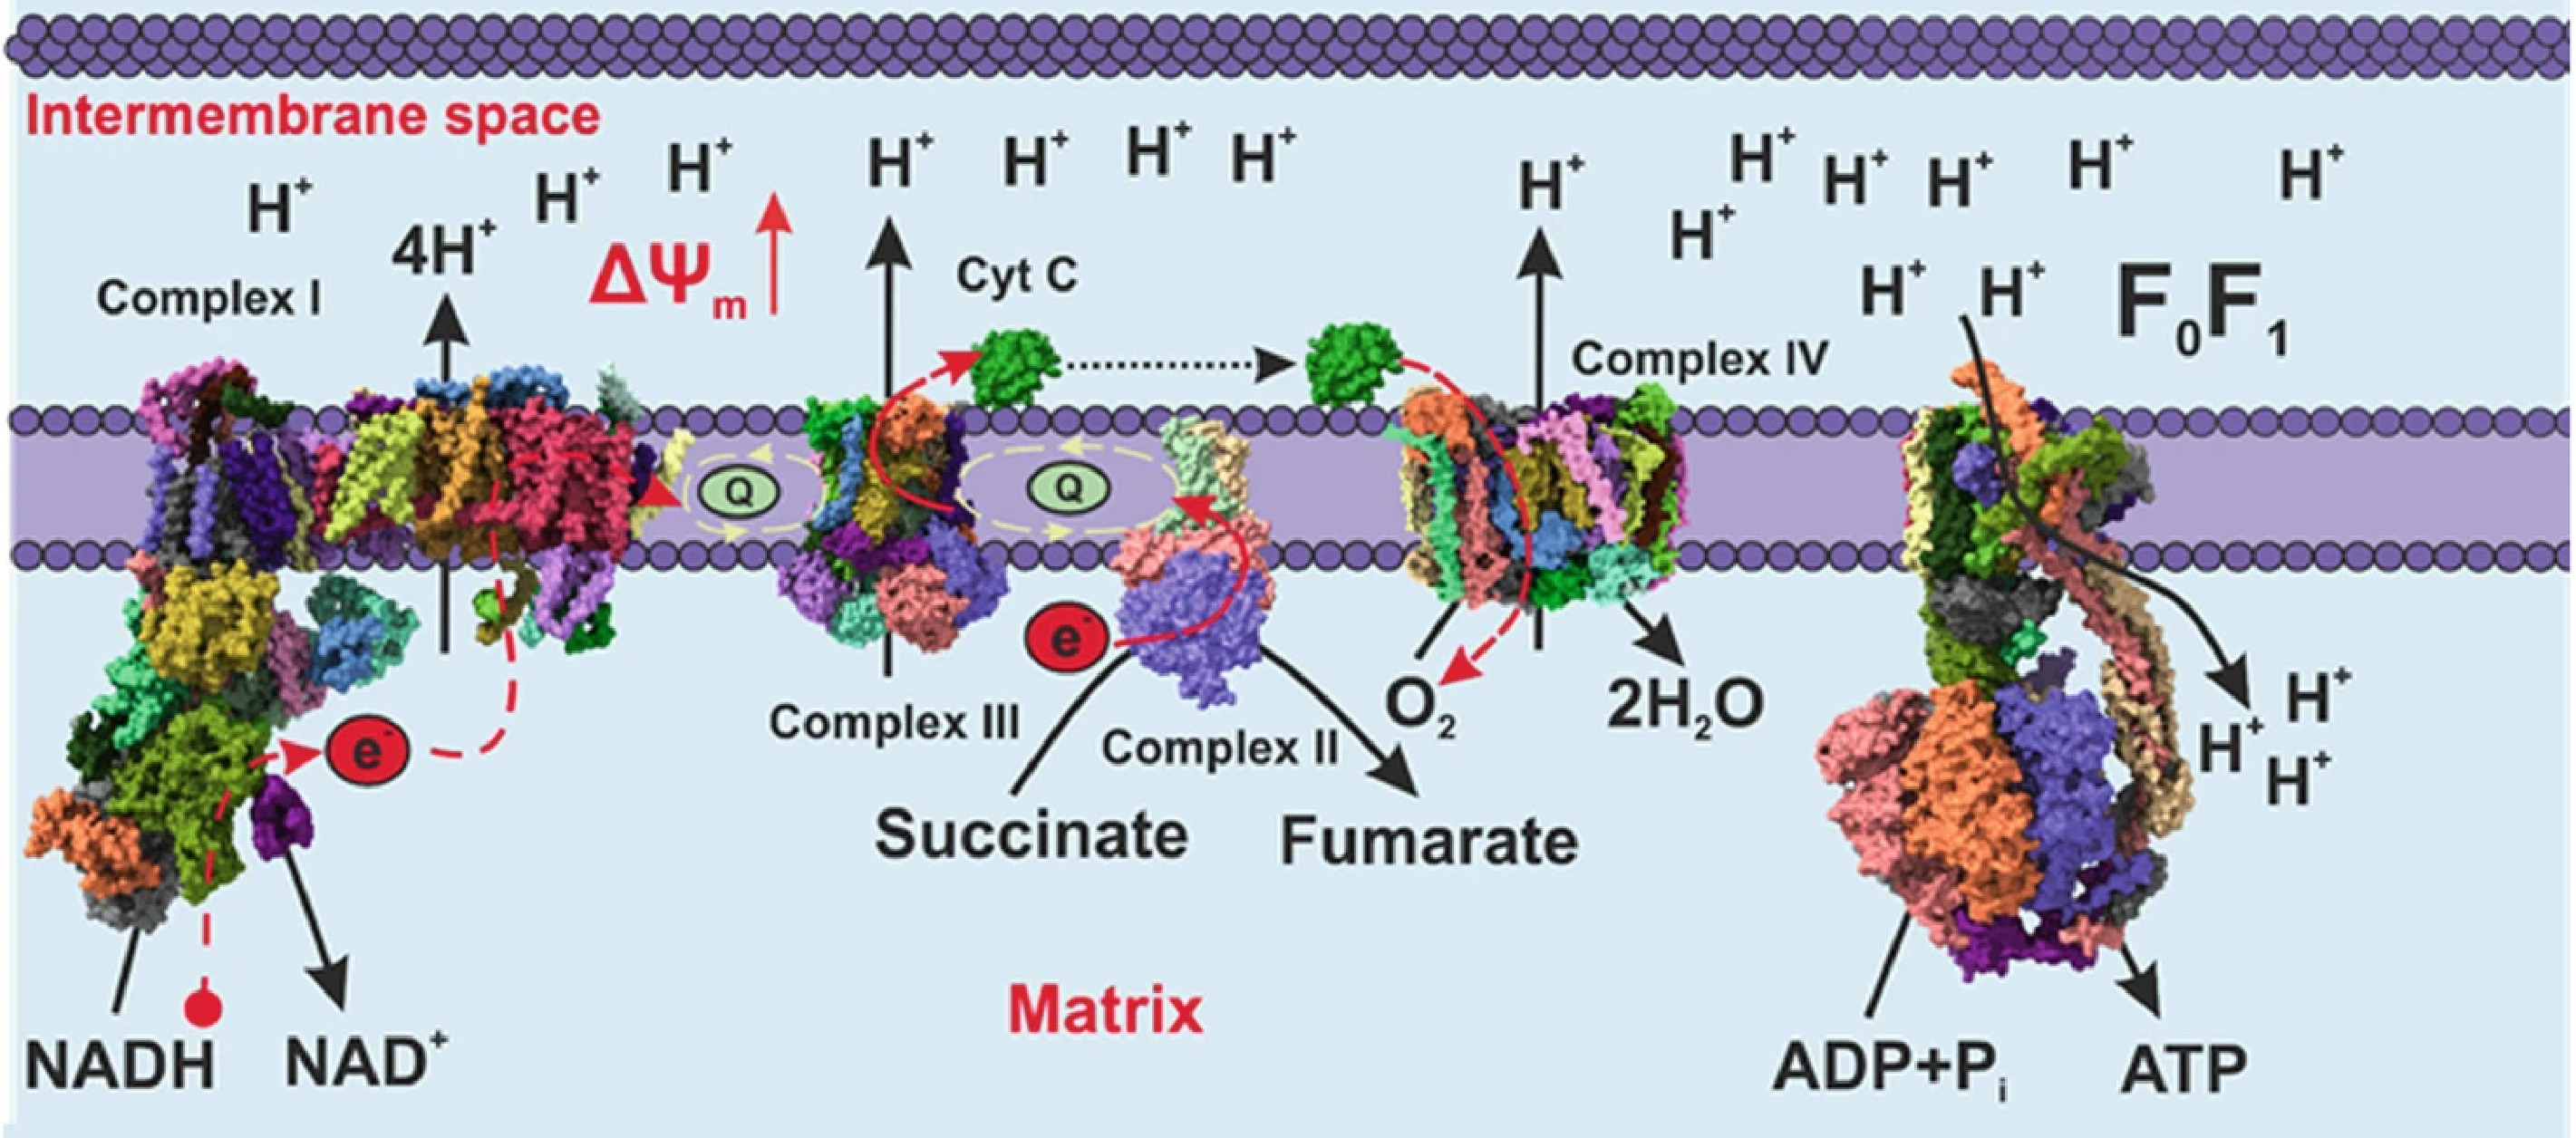
\includegraphics[width=0.95\textwidth]{Figures/1_Introduction/intro_atp_synthase.pdf}
    \caption{Electron transport chain coupled with oxidative phosphorylation in mitochondria. This figure was taken from \citep{baevInorganicPolyphosphateF0F1ATP2022}.}
    \label{fig:atp_synthase}
\end{figure}

Besides the F\textsubscript{1}-ATPase, other enzymes contribute to phosphate metabolism as well. In the context of \ac{polyp}, mammalian enzymes such as alkaline phosphatase (ALP) have demonstrated exopolyphosphatase activity, capable of hydrolysing \ac{polyp} chains of various lengths \citep{baevInorganicPolyphosphateF0F1ATP2022}.

The world of enzymes - and phosphate hydrolysis by F\textsubscript{1}-ATPase in particular - is both fascinating and complex. The F\textsubscript{1}-ATPase is a molecular machine capable of hydrolysing \ac{atp} and \ac{polyp}, yet the precise mechanism of hydrolysis remains not well understood. In order to address this gap, it is necessary to investigate the fundamental reaction mechanisms of phosphate hydrolysis, beginning with the simplest phosphate esters in less complex environments such as bulk water.



\section{Reaction mechanism: phosphate monoesters}
Computational and experimental studies have provided significant insights into the mechanisms of phosphate hydrolysis reactions. Various systems and methodologies have been employed to explore the details of these fundamental biological processes. The debate often centres on whether the reaction proceeds via an associative mechanism (bond formation precedes bond breaking) or a dissociative mechanism (bond breaking precedes bond formation), and the nature of the proton transfer.



\subsection{Phosphates} \label{subsec:phosphates}
Starting from the simplest possible system, it has been shown that the hydrolysis of \ac{memp} in water can proceed via either associative or concerted mechanisms \citep{kamerlinWhyNatureReally2013, kamerlinAssociativeDissociativeMechanisms2008, klahnMechanismHydrolysisPhosphate2006, duarteResolvingApparentConflicts2015}.

The associative mechanism may proceed in two ways: stepwise (A\textsubscript{N} + D\textsubscript{N}, where A\textsubscript{N} stands for nucleophilic addition and D\textsubscript{N} for nucleophilic departure) or concerted (A\textsubscript{N}D\textsubscript{N}). The stepwise mechanism involves two transition states and an intermediate. In contrast, the concerted mechanism proceeds through a single transition state without the formation of intermediates \citep{duarteResolvingApparentConflicts2015}.

\begin{figure}[b!]
    \centering
    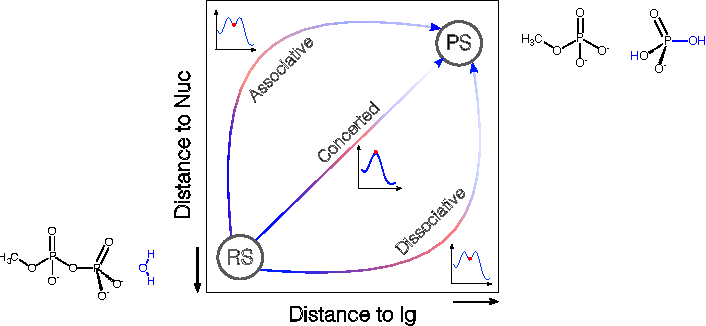
\includegraphics[width=0.95\textwidth]{Figures/1_Introduction/intro_mfj_plot.pdf}
    \caption{More O'Ferrall-Jencks (MFJ) plot of the possible reaction mechanisms for phosphate hydrolysis. The plot shows the free energy as a function of two reaction coordinates: the distance between phosphorus and the nucleophile (Nuc), and the distance between the leaving group (lg) and the phosphorus atom. RS stands for reactant state, PS for product state.}
    \label{fig:mfj_plot}
\end{figure}

In the case of the associative/stepwise mechanism (A\textsubscript{N} + D\textsubscript{N}, Figure~\ref{fig:reaction-mechanism}), the \ac{nuc} approaches the phosphorus atom while the \ac{lg} is still attached. Upon the nucleophile's approach, a concerted \ac{pt} occurs to one of the non-bridging oxygens. The reaction proceeds through a compact pentacoordinated transition state with a trigonal bipyramidal geometry, followed by a compact intermediate and the elimination of the leaving group in a subsequent transition state.

Regarding the associative/concerted mechanism (A\textsubscript{N}D\textsubscript{N}), it proceeds in a manner quite similar to the first step of the associative/stepwise pathway. The reaction also involves a compact transition state in which bond formation and bond cleavage occur simultaneously.

It has been shown that the protonation state of methyl phosphate lowers the overall barrier height of the rate-limiting step; however, it does not alter the reaction mechanism \citep{hassanEffectProtonationMechanism2017}. For the \ac{mehmp}, the calculated barrier height $\Delta G^{\ddagger}_{\text{calc}}$ is approximately 6-7 kcal/mol lower than that of the \ac{memp}. A similar effect was observed when OH\textsuperscript{-} acted as a nucleophile instead of a water molecule \citep{klahnMechanismHydrolysisPhosphate2006} (40 vs 47 kcal/mol, respectively). The latter fact arises a question about the proton-transfer in this reaction, for instance, whether it could happen in a concerted or a stepwise manner, in which the PT happens in the pre-equillibration phase.

For the associative mechanism, the barrier heights obtained from the quantum-mechanical calculations $\Delta G^{\ddagger}_{\text{calc}}$ lie in the range of 33.7-47.2 kcal/mol, while experimental values obtained at 25 \textdegree{C} range between 30.6 and 44.3 kcal/mol, depending on the protonation state. Detailed information about the calculated and experimentally determined barrier heights can be found in Table~\ref{tab:summary_comp_exp_barriers}. Corresponding data on transition state structures and intermediates is summarised in Table~\ref{tab:summary_ts_structures}.

\begin{figure}[b!]
    \centering
    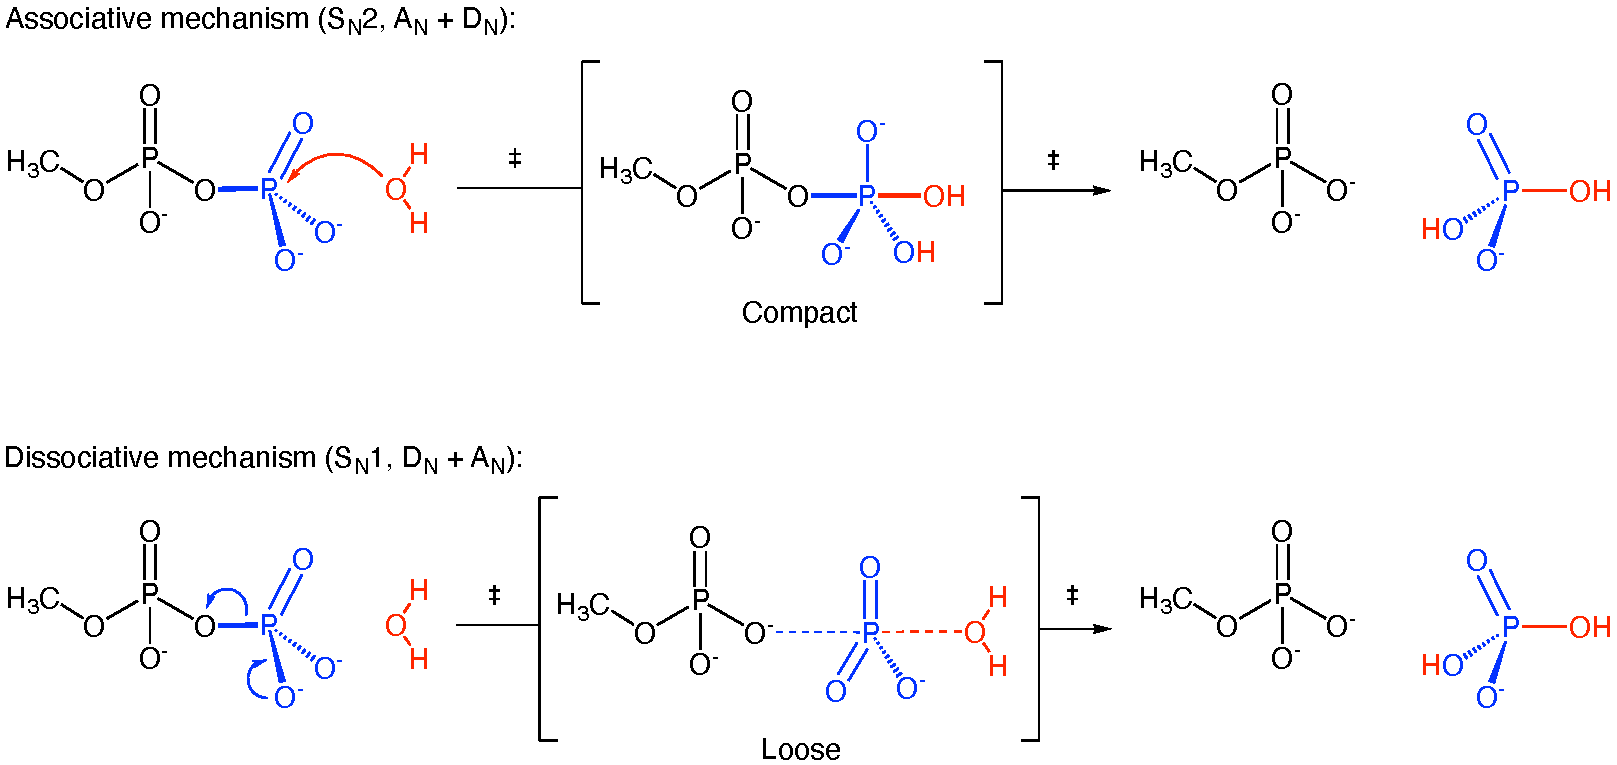
\includegraphics[width=0.95\textwidth]{Figures/1_Introduction/intro_reaction_mechanism.pdf}
    \caption{Associative and dissociative stepwise reaction mechanisms. The nucleophile (Nuc) is shown in red, the leaving group (lg) in black, and the phosphoryl group in blue.}
    \label{fig:reaction-mechanism}
\end{figure}

The concerted mechanism (A\textsubscript{N}D\textsubscript{N}) is characterised by a single transition state \; where the nucleophile approaches the phosphorus atom while the leaving group remains attached. The reaction proceeds via a compact pentacoordinated transition state with a trigonal bipyramidal geometry, which is more loose compared to that of the associative mechanism (Table~\ref{tab:summary_ts_structures}). In this transition state, the distance between the phosphorus atom and the nucleophile is approximately 2.06-2.75~\AA, while the distance between the leaving group and the phosphorus atom is around 2.61-2.75~\AA. The barrier heights for the concerted mechanism are 44-44.5 kcal/mol depending on the level of theory used in calculations and the number of water molecules in the system (Table~\ref{tab:summary_comp_exp_barriers}).

As can be observed, it is rather difficult to clearly distinguish between the associative and concerted mechanisms, and it appears that both may occur in bulk water. Even by looking at the activation entropies of both reaction pathways, it's clear that the corresponding values are similarly small: 0.7 and -1.6 kcal/mol for the associative and concerted mechanisms, respectively \citep{duarteResolvingApparentConflicts2015}.  Nevertheless, the dissociative mechanism is unlikely to take place, or at least it has not been observed.



\subsection{Diphosphates} \label{subsec:diphosphates_reaction_mechanism}
Moving on to more complex systems, the hydrolysis of pyrophosphates (diphosphates) (e.g., \ac{medp}), which are the main focus of this thesis, has also been thoroughly studied. It has been shown that the reaction mechanism can proceed through either associative or concerted pathways, just as in the case of methyl phosphate. However, there is a twist to this story: the dissociative mechanism has also been proposed to take place \citep{klahnMechanismHydrolysisPhosphate2006, kamerlinAssociativeDissociativeMechanisms2008, prasadAddressingOpenQuestions2013}. A schematic representation of these mechanisms is presented in Figure~\ref{fig:mfj_plot}, which illustrates the \ac{mfj}. The MFJ plot is a useful two-dimensional graphical representation of multidimensional free energy surfaces.

In the associative/concerted mechanism, the reaction undergoes the same steps as discussed in Subsection~\ref{subsec:phosphates}. The transition state has a similarly compact geometry: the distance between the phosphorus atom and the nucleophile is approximately 2.03--2.26~\AA, and the distance between the leaving group and the phosphorus atom is around 1.82--2.4~\AA, as shown in Table~\ref{tab:summary_ts_structures}. However, the calculated barrier heights are slightly lower in comparison to methyl phosphate, ranging from 34 to 38 kcal/mol (Table~\ref{tab:summary_comp_exp_barriers}).

\begin{table}[htbp]
    \centering
    \small
    \caption{Summary of computational and experimental studies on phosphate hydrolysis. In the case of calculated $\Delta G^\ddagger$, the predicted rate-limiting step is given. \textsuperscript{1}The values were calculated using \ac{tst}.}
    \label{tab:summary_comp_exp_barriers}
    \resizebox{\textwidth}{!}{%
    \renewcommand{\arraystretch}{1.3}
    \begin{tabular}{@{}p{4.5cm} p{2.5cm} p{4.0cm} p{3.0cm} p{3.0cm} p{1.0cm}@{}}
    \toprule
    \textbf{System} & \textbf{Method} & \textbf{Level of theory} & \textbf{Mechanism} & \textbf{\boldmath$\Delta G^\ddagger$ (kcal/mol)} & \textbf{Ref.} \\ \midrule
    
    MeMP$^{2-}$ + H$_2$O & 
    DFT & B3LYP/6-311+G** and COSMO &
    Associative \newline Concerted & 
    47.2 \newline 44.5 & 
    \citep{kamerlinAssociativeDissociativeMechanisms2008} \\
    
    MeMP$^{2-}$ + H$_2$O & 
    DFT & B3LYP/6-311++G** and COSMO & 
    Associative & 
    47 & 
    \citep{klahnMechanismHydrolysisPhosphate2006} \\
    
    MeMP$^{2-}$ + 3 H$_2$O & 
    DFT & M06-2X/6-311+G** and SMD &
    Associative \newline Concerted & 
    $\approx$ 36 \newline $\approx$ 44 & 
    \citep{duarteResolvingApparentConflicts2015} \\
    
    MeMP$^{2-}$ + 4 H$_2$O & 
    DFT & M06-2X/6-311+G** &
    Associative & 
    $\approx$ 40.8$\pm$1.9 & 
    \citep{hassanEffectProtonationMechanism2017} \\
    
    MeHMP$^{-}$ + 4 H$_2$O & 
    DFT & M06-2X/6-311+G** &
    Associative & 
    $\approx$ 33.7$\pm$1.7 & 
    \citep{hassanEffectProtonationMechanism2017} \\
    
    MeDP$^{3-}$ + 2 H$_2$O & 
    DFT & B3LYP/6-311++G** and PCM & 
    Associative \newline Dissociative & 
    34.64 \newline 35.24 & 
    \citep{prasadAddressingOpenQuestions2013} \\
    
    MeDP$^{3-}$ + H$_2$O & 
    DFT & B3LYP/6-311+G** and COSMO & 
    Associative \newline Dissociative & 
    34.8 \newline 30.3 & 
    \citep{kamerlinAssociativeDissociativeMechanisms2008} \\
    
    MeDP$^{3-}$ + H$_2$O & 
    DFT & B3LYP/6-311++G** and COSMO & 
    Associative \newline Concerted & 
    38 \newline 34 & 
    \citep{klahnMechanismHydrolysisPhosphate2006} \\
    
    MeHDP$^{2-}$ + H$_2$O & 
    DFT & B3LYP/6-311++G** and COSMO & 
    Associative \newline Concerted & 
    34 \newline 31 & 
    \citep{klahnMechanismHydrolysisPhosphate2006} \\
    
    MeDP$^{3-}$ + Mg$^{2+}$ + 5 H$_2$O & 
    QM/MM, \newline FEP (EVB) & B3LYP/6-311++G** and MM & 
    Associative \newline Concerted \newline Dissociative & 
    35 \newline 34 \newline 35 & 
    \citep{klahnMechanismHydrolysisPhosphate2006} \\

    MeTP$^{4-}$ + Mg$^{2+}$ + 54 H$_2$O & 
    CPMD & PBE/PW with Troullier-Martins pseudopotentials & 
    Associative \newline Concerted \newline Dissociative & 
    39.1 \newline 35.1 \newline 36.6 & 
    \citep{akolaATPHydrolysisWater2003} \\
    
    MeTP$^{4-}$ + Mg$^{2+}$ + 113 H$_2$O & 
    BOMD, \newline metadynamics & BLYP/TZV2P with GTH pseudopotentials & 
    Associative \newline Concerted & 
    29 \newline 29-30 & 
    \citep{glavesMechanisticInsightsHydrolysis2012} \\

    ATP$^{4-}$ + Mg$^{2+}$ + 4163 H$_2$O + counterions & 
    QM/MM, NEB & B3LYP/6-311++G** and MM & 
    Concerted & 
    32.5 & 
    \citep{wangQMMMInvestigation2015} \\
    
    ATP$^{4-}$ + Mg$^{2+}$ + 1800 H$_2$O + counterions & 
    QM/MM, QM = CPMD & BLYP/PW with Troullier-Martins pseudopotentials and MM & 
    Associative \newline Dissociative & 
    36.2 \newline 33.4 & 
    \citep{harrisonQuantumClassicalDynamics2012} \\
    
    \midrule
    
    Methyl phosphate \newline dianion & 
    Exp. at 25\textdegree{C} & 
    -- & -- & 
    44.3 & 
    \citep{wolfendenDegreesDifficultyWaterConsuming2006} \\
    
    Methyl phosphate \newline monoanion & 
    Exp. at 25\textdegree{C} & 
    -- & -- & 
    30.6 & 
    \citep{wolfendenDegreesDifficultyWaterConsuming2006} \\
    
    Pyrophosphate trianion & 
    Exp. at 25\textdegree{C} & 
    -- & -- & 
    29.2 & 
    \citep{wolfendenDegreesDifficultyWaterConsuming2006} \\
    
    Pyrophosphate dianion & 
    Exp. at 25\textdegree{C} & 
    -- & -- & 
    27.7 & 
    \citep{wolfendenDegreesDifficultyWaterConsuming2006} \\
    
    ADP$^{2-}$ (or ATP$^{3-}$) & 
    Exp. at 25\textdegree{C} & 
    -- & -- & 
    27.5 & 
    \citep{wolfendenDegreesDifficultyWaterConsuming2006} \\
    
    ATPH$^{3-}$ (or ATP$^{4-}$) & 
    Exp. at 70\textdegree{C} & 
    pH=6.69-7.66 & -- & 
    24.34-24.78\textsuperscript{1} & 
    \citep{ramirezMagnesiumCalciumIon1980} \\
    
    dADPH$^{2-}$ (or dADP$^{3-}$) & 
    Exp. at 70\textdegree{C} & 
    pH=6.82 & -- & 
    24.25\textsuperscript{1} & 
    \citep{ramirezComparativeStudyHydrolysis1982a} \\
    
    dATPH$^{3-}$ (or dATP$^{4-}$) & 
    Exp. at 70\textdegree{C} & 
    pH=7.00  & -- & 
    24.50\textsuperscript{1} & 
    \citep{ramirezComparativeStudyHydrolysis1982a} \\
    
    MgATPH$^{-}$ (or MgATP$^{2-}$) & 
    Exp. at 70\textdegree{C} & 
    pH=6.59-7.63  & -- & 
    24.59-24.64\textsuperscript{1} & 
    \citep{ramirezMagnesiumCalciumIon1980} \\
    
    CaATPH$^{-}$ (or CaATP$^{2-}$) & 
    Exp. at 70\textdegree{C} & 
    pH=6.67-7.01 & -- & 
    25.71-25.72\textsuperscript{1} & 
    \citep{ramirezMagnesiumCalciumIon1980} \\
    
    \bottomrule
    \end{tabular}%
    }
\end{table}

The concerted pathway is characterised by the same general mechanism as discussed in Subsection~\ref{subsec:phosphates}. The transition state is more expansive than in the associative mechanism, with the distance between the phosphorus atom and the nucleophile being approximately 2.26--2.5~\AA, while the distance between the leaving group and the phosphorus atom is around 2.7~\AA\ (Table~\ref{tab:summary_ts_structures}). The barrier heights for the concerted mechanism are 31 and 34 kcal/mol (Table~\ref{tab:summary_comp_exp_barriers}), which is notably lower than in the case of methyl phosphate.

In general, it can be noted that the barrier height is strongly dependent on the $pK_a$ value of the leaving group. The lower the $pK_a$, the lower the $\Delta G^{\ddagger}$ ($pK_a$(CH\textsubscript{3}O\textsuperscript{-}) $= 15.5$ vs $pK_a$(CH\textsubscript{3}PO\textsubscript{4}\textsuperscript{2-}) $= 6.3$). Not only does a lower $pK_a$ reduce the barrier height, but it also favours the mechanisms towards the dissociative pathway on the spectrum of associative/stepwise-concerted-dissociative/stepwise mechanisms \citep{klahnMechanismHydrolysisPhosphate2006}.

The dissociative mechanism can proceed via both concerted and stepwise routes. The dissociative/concerted pathway is quite similar to the general concerted mechanism. The main difference lies in the synchrony of the transition state: while the general concerted mechanism has a more synchronous transition state, the dissociative/concerted is asynchronous and features a greater distance between the phosphorus atom and the leaving group.

On the other hand, the dissociative/stepwise pathway (D\textsubscript{N} + A\textsubscript{N}) is characterised by the departure of the leaving group from the phosphorus atom in the first saddle point. Thus, there is no bond remaining between the phosphorus and the leaving group. Following the departure of the leaving group, a planar metaphosphate PO\textsubscript{3}\textsuperscript{-} is formed, as illustrated in Figure~\ref{fig:reaction-mechanism}. The transition state is more loose compared to that of the associative mechanism, with the distance between the phosphorus atom and the nucleophile being 2.7~\AA, and the distance between the leaving group and the phosphorus atom being 3.4~\AA\ (Table~\ref{tab:summary_ts_structures}). Consequently, after TS\textsubscript{1}, the system reaches an intermediate step in which the nucleophile is positioned closer to the metaphosphate, followed by a nucleophile attack and bond formation in TS\textsubscript{2}.

Calculated barrier heights for the dissociative mechanism lie in the range of 30.3-35.24 kcal/mol (Table~\ref{tab:summary_comp_exp_barriers}), which is lower than those for any of the previously mentioned mechanisms. By comparing the calculated and experimentally obtained $\Delta G^{\ddagger}$, one could notice that the dissociative mechanism is more favourable than the associative and concerted ones. The $\Delta G^{\ddagger}_{\text{exp}}$ values for the pyrophosphate trianion and dianion are 29.2 and 27.7 kcal/mol, respectively. The influence of one-water (1W) or two-water (2W) mechanisms has also been explored \citep{prasadAddressingOpenQuestions2013}, but the overall barriers remain similar.

The dissociative mechanism is further favoured by the presence of metal ions, such as Mg\textsuperscript{2+}, as well as in cases where \ac{medp} is protonated, i.e. \ac{mehdp}. Interestingly, in the latter case, the proton always transfers to the leaving group en route to the product state \citep{klahnMechanismHydrolysisPhosphate2006}.

\begin{table}[htbp]
    \centering
    \small
    \caption{Summary of the distances between the phosphorus atom and the nucleophile as well as the leaving group in the transition states and intermediates. All distances are in \AA.}
    \label{tab:summary_ts_structures}
    \resizebox{\textwidth}{!}{%
    \renewcommand{\arraystretch}{1.2}
    \begin{tabular}{@{}p{2.0cm} p{2.0cm} 
                    >{\centering\arraybackslash}p{2.16cm} 
                    >{\centering\arraybackslash}p{2.16cm} 
                    >{\centering\arraybackslash}p{2.16cm} 
                    >{\centering\arraybackslash}p{2.16cm} 
                    >{\centering\arraybackslash}p{2.16cm} 
                    >{\centering\arraybackslash}p{2.16cm} 
                    p{1.0cm}@{}}
    \toprule
    \textbf{System} & \textbf{Mechanism} & 
    \multicolumn{2}{c}{\textbf{TS\textsubscript{1}}} & 
    \multicolumn{2}{c}{\textbf{Intermediate}} & 
    \multicolumn{2}{c}{\textbf{TS\textsubscript{2}}} & 
    \textbf{Ref.} \\
    \cmidrule(lr){3-4} \cmidrule(lr){5-6} \cmidrule(lr){7-8}
    & & \textbf{d(P-O\textsubscript{Nuc})} & \textbf{d(P-O\textsubscript{lg})} & 
            \textbf{d(P-O\textsubscript{Nuc})} & \textbf{d(P-O\textsubscript{lg})} & 
            \textbf{d(P-O\textsubscript{Nuc})} & \textbf{d(P-O\textsubscript{lg})} & \\ 
    \midrule

    MeMP$^{2-}$ & 
    Associative (A\textsubscript{N}D\textsubscript{N}) & 
    2.0 & 1.8 & 
    -- & -- & 
    -- & -- & 
    \citep{klahnMechanismHydrolysisPhosphate2006} \\

    & 
    Associative (A\textsubscript{N}D\textsubscript{N}) & 
    1.9 & 2.15 & 
    -- & -- & 
    -- & -- & 
    \citep{kamerlinAssociativeDissociativeMechanisms2008} \\

    & 
    Associative (A\textsubscript{N} + D\textsubscript{N}) & 
    2.16 & 1.71 & 
    1.84 & 1.78 & 
    1.71 & 2.24 & 
    \citep{duarteResolvingApparentConflicts2015} \\

    & 
    Associative (A\textsubscript{N} + D\textsubscript{N}) & 
    2.08 & 1.78 & 
    1.99 & 1.80 & 
    1.77 & 2.52 & 
    \citep{hassanEffectProtonationMechanism2017} \\

    & 
    Concerted (A\textsubscript{N}D\textsubscript{N}) & 
    2.75 & 2.75 & 
    -- & -- & 
    -- & -- & 
    \citep{kamerlinAssociativeDissociativeMechanisms2008} \\

    & 
    Concerted (A\textsubscript{N}D\textsubscript{N}) & 
    2.06 & 2.61 & 
    -- & -- & 
    -- & -- & 
    \citep{duarteResolvingApparentConflicts2015} \\

    MeHMP$^{-}$& 
    Associative (A\textsubscript{N} + D\textsubscript{N}) & 
    2.26 & 1.66 & 
    1.76 & 1.77 & 
    1.68 & 2.25 & 
    \citep{hassanEffectProtonationMechanism2017} \\

    \midrule

    MeDP$^{3-}$& 
    Associative (A\textsubscript{N}D\textsubscript{N}) & 
    2.2 & 2.0 & 
    -- & -- & 
    -- & -- & 
    \citep{kamerlinAssociativeDissociativeMechanisms2008} \\

    & 
    Associative (A\textsubscript{N}D\textsubscript{N}) & 
    2.03 & 1.88 & 
    -- & -- & 
    -- & -- & 
    \citep{klahnMechanismHydrolysisPhosphate2006} \\
    
    & 
    Associative (A\textsubscript{N}D\textsubscript{N}) & 
    2.2 & 2.0 & 
    -- & -- & 
    -- & -- & 
    \citep{prasadAddressingOpenQuestions2013} \\

    &
    Concerted (A\textsubscript{N}D\textsubscript{N}) & 
    2.5 & 2.7 & 
    -- & -- & 
    -- & -- & 
    \citep{klahnMechanismHydrolysisPhosphate2006} \\

    & 
    Dissociative (A\textsubscript{N}D\textsubscript{N}) & 
    2.8 & 3.25 & 
    -- & -- & 
    -- & -- & 
    \citep{kamerlinAssociativeDissociativeMechanisms2008} \\

    & 
    Dissociative (D\textsubscript{N} + A\textsubscript{N}) & 
    2.7 & 3.4 & 
    2.0 & 3.75 & 
    1.7 & 3.75 & 
    \citep{prasadAddressingOpenQuestions2013} \\

    MeDP$^{3-}$ \newline + Mg$^{2+}$ &
    Associative (A\textsubscript{N}D\textsubscript{N}) &
    2.1 & 2.4 & 
    -- & -- & 
    -- & -- & 
    \citep{klahnMechanismHydrolysisPhosphate2006} \\

    &
    Concerted (A\textsubscript{N}D\textsubscript{N}) &
    2.3 & 2.7 & 
    -- & -- & 
    -- & -- & 
    \citep{klahnMechanismHydrolysisPhosphate2006} \\

    &
    Dissociative (A\textsubscript{N}D\textsubscript{N}) &
    2.8 & 3.4 & 
    -- & -- & 
    -- & -- & 
    \citep{klahnMechanismHydrolysisPhosphate2006} \\

    MeHDP$^{2-}$& 
    Associative (A\textsubscript{N}D\textsubscript{N}) & 
    2.26 & 1.82 & 
    -- & -- & 
    -- & -- & 
    \citep{klahnMechanismHydrolysisPhosphate2006} \\

    &
    Concerted (A\textsubscript{N}D\textsubscript{N}) & 
    2.26 & 2.78 & 
    -- & -- & 
    -- & -- & 
    \citep{klahnMechanismHydrolysisPhosphate2006} \\
    
    \midrule

    MeTP$^{4-}$ \newline + Mg$^{2+}$&
    Associative (A\textsubscript{N}D\textsubscript{N}) & 
    1.9 & 2.0 & 
    -- & -- & 
    -- & -- & 
    \citep{akolaATPHydrolysisWater2003} \\

    & Associative (A\textsubscript{N} + D\textsubscript{N}) & 
    2.03 & 3.11 & 
    1.95 & 3.06 & 
    1.66 & 3.26 & 
    \citep{glavesMechanisticInsightsHydrolysis2012} \\

    &
    Concerted (A\textsubscript{N}D\textsubscript{N}) & 
    2.5 & 2.6 & 
    -- & -- & 
    -- & -- & 
    \citep{akolaATPHydrolysisWater2003} \\

    &
    Concerted (A\textsubscript{N}D\textsubscript{N}) & 
    2.28 & 2.69 & 
    -- & -- & 
    -- & -- & 
    \citep{glavesMechanisticInsightsHydrolysis2012} \\

    &
    Dissociative (A\textsubscript{N}D\textsubscript{N}) & 
    3.6 & 3.5 & 
    -- & -- & 
    -- & -- & 
    \citep{akolaATPHydrolysisWater2003} \\

    ATP$^{4-}$ \newline + Mg$^{2+}$ &
    Associative (A\textsubscript{N}D\textsubscript{N}) & 
    1.9 & 1.9 & 
    -- & -- & 
    -- & -- & 
    \citep{harrisonQuantumClassicalDynamics2012} \\
    
    &
    Concerted (A\textsubscript{N}D\textsubscript{N}) & 
    2.8 & 3.2 & 
    -- & -- & 
    -- & -- & 
    \citep{wangQMMMInvestigation2015} \\

    &
    Dissociative (A\textsubscript{N}D\textsubscript{N}) & 
    3.5 & 3.5 & 
    -- & -- & 
    -- & -- & 
    \citep{wangQMMMInvestigation2015} \\

    \bottomrule
    \end{tabular}%
    }
\end{table}

Even though computational studies suggest that Mg\textsuperscript{2+} promotes the dissociative mechanism, experimental data do not support this hypothesis \citep{ramirezMagnesiumCalciumIon1980}, since the $\Delta G^{\ddagger}_{\text{exp}}$ obtained at 70\textdegree{C} shows little to no difference, at least in the case of adenosine triphosphate (Table~\ref{tab:summary_comp_exp_barriers}).



\subsection{Triphosphates}
Last but not least, let us consider the hydrolysis of triphosphates. These systems more closely resemble the molecules, e.g., \ac{atp}, that are in charge of energy metabolism in all living organisms.

The hydrolysis of \ac{metp} and \ac{atp} has been studied using a range of computational methods. It has been shown that the reaction mechanisms share many similarities with those observed in mono- and diphosphates. Specifically, the mechanism may proceed via associative/concerted and associative/stepwise routes, as well as concerted and dissociative/concerted pathways (Table~\ref{tab:summary_ts_structures}). 

When comparing the calculated and experimentally obtained $\Delta G^{\ddagger}$ values, it is difficult to clearly distinguish between the aforementioned mechanisms. The calculated barrier heights span a range from 29 to 39.1 kcal/mol, whereas experimental data suggest that the barrier height for ATP should be around 27.5 kcal/mol, as shown in Table~\ref{tab:summary_comp_exp_barriers}. The more complex the system becomes, the more factors one must likely take into account.

In summary, computational investigations reveal a nuanced and peculiar picture of phosphate hydrolysis. The preferred mechanism (associative, concerted, or dissociative) and the proton transfer route (1W, 2W, etc.) depend significantly on specific factors such as the pKa of the leaving group, the protonation state, the presence of metal ions like Mg$^{2+}$, and the surrounding solvent environment.

While the studies discussed in the sections above provide valuable insights into the reaction mechanism of phosphate hydrolysis, they suffer from several weaknesses. First, the majority of these studies are based on small model systems containing a substrate and a handful of water molecules, with calculations conducted in the gas phase or using an implicit solvent model. Such systems lack important interactions with the bulk solvent, which are crucial for processes like proton transfer via the water network. Moreover, the free energy surface scans often cover only a limited number of points, resulting in poor sampling of the configurational space.

Second, in \ac{bomd} and \ac{cpmd} studies, the simulation lengths were limited to a few hundred picoseconds at most, which is insufficient to yield converged free energy surfaces and, consequently, to get accurate kinetics and thermodynamics of the reaction.

Limitations of previous studies highlight the need for a more comprehensive investigation of the reaction mechanism of methyl diphosphate hydrolysis in water, and serve as a motivation for revisiting phosphate hydrolysis in this thesis.



\section{Research goals}

To properly study the underlying free energy surface of the reaction mechanism, adequate sampling of the configurational space is crucial. To achieve this, various free energy techniques, such as metadynamics, can be employed - provided that the level of theory is sufficient to describe a system of realistic size while allowing results to be obtained within a reasonable timeframe. This is precisely the goal of the present project.

As a model system, methyl diphosphate hydrolysis in water has been chosen. Methyl diphosphate is a relatively simple phosphate ester that can represent more complex molecules like \ac{adp} and \ac{atp}. The main focus of this thesis is to investigate the reaction mechanism of \ac{medp} hydrolysis in water using well-tempered metadynamics, and to explore the influence of the protonation state and the solvent environment on the reaction mechanism. To run the metadynamics simulations, a neural network potential will be trained, thus allowing \textit{ab initio} molecular dynamics simulations to be performed at low computational cost.

Specifically, the following goals have been set for this thesis:
\begin{itemize}
    \item Compose a comprehensive dataset of molecular configurations covering all steps of the methyl diphosphate hydrolysis reaction mechanism.
    \item Train the NequIP neural network to fit a neural network potential that serves as an engine for the \textit{ab initio} molecular dynamics simulations.
    \item Assess the accuracy and performance of the neural network potential with respect to network complexity and the size of the training set.
    \item Perform extensive well-tempered metadynamics simulations to obtain the free energy surface of the methyl diphosphate hydrolysis reaction mechanism.
    \item Gain insights into the reaction mechanism, i.e. the kinetics and thermodynamics of the reaction, and compare the results with previously published data.
    \item Gain insights into the proton transfer mechanism.
\end{itemize}

Taking the above-mentioned goals into account, the present thesis follows the idea of Paul A. M. Dirac~\citep{diracQuantumMechanicsManyelectron1997}, who emphasised the need for approximate practical methods in quantum mechanics to explain complex atomic systems without excessive computational demands: 

\begin{displayquote}
    The underlying physical laws necessary for the mathematical theory of a large part of physics and the whole of chemistry are thus completely known, and the difficulty is only that the exact application of these laws leads to equations much too complicated to be soluble. \textit{It therefore becomes desirable that approximate practical methods of applying quantum mechanics should be developed, which can lead to an explanation of the main features of complex atomic systems without too much computation.}
\end{displayquote}

The use of neural network potentials in this thesis aims to achieve precisely that: to provide a practical and efficient approach to studying the reaction mechanism while maintaining a high level of accuracy.

\chapter{Theory}

\section{A brief introduction to statistical mechanics}
The discussion in this section is mostly based on the ``Introduction to Computational Chemistry'' textbook written by Jensen~\citep{jensenIntroductionComputationalChemistry2017}, ``Statistical Mechanics: Theory and Molecular Simulation'' by Tuckermann~\citep{tuckermanStatisticalMechanicsTheory2023}, and ``Understanding Molecular Simulation: From Algorithms to Applications'' by Frenkel and Smit~\citep{frenkelUnderstandingMolecularSimulation2002} unless stated otherwise.



\subsection{Partition functions}
The development of the field of statistical mechanics has been crucial for the computational chemistry community, as it enables the connection between the jigglings and wigglings of atoms and the properties of much larger systems such as liquids and solids.

Let us begin with the most fundamental concept: the partition function. The partition function is akin to a Swiss army knife in statistical mechanics, meaning it is a versatile tool that makes the connection between microscopic and macroscopic properties in thermodynamics possible. In the simplest case of a single molecule, the partition function $q$ takes the following form:

\begin{equation}
    q = \sum_{i = \text{levels}}^{\infty} g_i e^{-\epsilon_i/kT}
\end{equation}

Here, it is expressed as a sum over all energy levels $\epsilon_i$ of a molecule (or particle), multiplied by a degeneracy factor $g_i$ in cases where multiple levels have the same energy. The term $kT$ represents the Boltzmann factor.

Moving on to a more complex scenario in which the partition function describes multiple molecules, we arrive at the partition function $Q$ for non-interacting particles, such as those in an ideal gas:

\begin{equation}
    \label{eq:Q_noninteracting}
    Q = q^N \; \text{(different particles)} \quad Q = \frac{q^N}{N!} \; \text{(identical particles)}
\end{equation}

Here, $N$ denotes the total number of particles. However, one could argue that if we wish to describe a real system such as bulk water, we must account for interactions between molecules. Consequently, Equation~\ref{eq:Q_noninteracting} must be rewritten:

\begin{equation}
    Q = \sum_{i}^{\infty} e^{-E_i/kT}
\end{equation}

In this case, the partition function $Q$ includes contributions from all possible energy states $E_i$ of the system.

Although the concept of the partition function might initially appear abstract, it can be clarified by expressing it in a different form, namely, within the context of the \ac{rrho} approximation, where the electronic, vibrational, and rotational degrees of freedom can be separated. For a single molecule case it would look like:

\begin{equation}
    q_{\text{tot}} = q_{\text{trans}} \times q_{\text{rot}} \times q_{\text{vib}} \times q_{\text{elec}}
\end{equation}

Let us now examine each contribution in more detail. From this point onward we will consider polyatomic molecules in the formulation of the partition functions, unless stated otherwise.

The translational partition function $q_\text{trans}$ can be derived from the energy expression for a particle in a one-dimensional box and is given by:

\begin{equation}
    q_{\text{trans}} = \left(\frac{2\pi MkT}{h^2}\right)^{3/2} V
\end{equation}

Here, $M$ is the total molecular mass, and $V$ is the volume. Turning to the rotational partition function $q_\text{rot}$, it can be derived from the Schr\"odinger equation for a diatomic "rigid rotor" and has the following form:

\begin{equation}
    q_{\text{rot}} = \frac{8\pi^2IkT}{h^2\sigma}
\end{equation}

In this expression, $I$ denotes the moment of inertia, and $\sigma$ represents the symmetry factor, i.e. the order of the rotational subgroup within the molecular point group. For polyatomic molecules, writing an exact expression is more complex, but an approximate form can be used:

\begin{equation}
    q_{\text{rot}} = \frac{\sqrt{\pi}}{\sigma}\left(\frac{8\pi^2kT}{h^2}\right)^{3/2} \sqrt{I_1I_2I_3}
\end{equation}

For the vibrational partition function $q_\text{vib}$, it is expressed as a product over the various vibrational modes of a molecule, each with frequency $\nu_i$:

\begin{equation}
    q_{\text{vib}} = \prod_{i} \frac{e^{-h\nu_i/2kT}}{1-e^{-h\nu_i/kT}}
\end{equation}

Lastly, the electronic partition function $q_\text{elec}$ is given as a sum over all electronic states of a molecule, from the ground state to all excited states. However, since the energy difference between the ground state and higher states is usually much greater than $kT$ at ambient temperatures, the function can typically be approximated by considering only the ground state:

\begin{equation}
    q_{\text{elec}} = \sum_{i=0}^{\infty} g_i e^{-\epsilon_i/kT} \approx g_0 e^{-\epsilon_0/kT}
\end{equation} 



\subsection{Macroscopic properties and thermodynamic functions}

Once the partition function is determined, it provides a direct means of evaluating macroscopic properties. For instance, the internal energy $U$ and the Helmholtz free energy $A$ can be calculated from the partition function $Q$:

\begin{align}
    U &= kT^2 \left(\frac{\partial \ln Q}{\partial T}\right)_V \\
    A &= -kT\ln Q
\end{align}

In addition, other macroscopic properties, such as pressure $P$ and the heat capacity at constant volume $C_V$, can also be expressed in terms of the partition function:

\begin{align}
    P &= -\left(\frac{\partial A}{\partial V}\right)_T = kT\left(\frac{\partial \ln Q}{\partial V}\right)_T \\
    C_V &= \left(\frac{\partial U}{\partial T}\right)_V = 2kT\left(\frac{\partial \ln Q}{\partial T}\right)_V + kT^2\left(\frac{\partial^2 \ln Q}{\partial T^2}\right)_V
\end{align}

Turning to thermodynamic functions, namely enthalpy $H$, entropy $S$, and Gibbs free energy $G$, these can also be derived from the partition function $Q$:

\begin{align}
    H &= U + PV = kT^2\left(\frac{\partial \ln Q}{\partial T}\right)_V + kTV\left(\frac{\partial \ln Q}{\partial V}\right)_T \\
    S &= \frac{U-A}{T} = kT\left(\frac{\partial \ln Q}{\partial T}\right)_V + k\ln Q \\
    G &= H - TS = kTV\left(\frac{\partial \ln Q}{\partial V}\right)_T - kT\ln Q
\end{align}

This connection between macroscopic observables, thermodynamic functions, and the partition function once again highlights its fundamental importance in statistical thermodynamics.



\subsection{The canonical ensemble}
Having established a method to calculate the macroscopic properties of a system we implicitly relied on averaging over a large enough number of states. Therefore one may naturally ask: how can we sample enough configurations to apply the equations described in the previous section under conditions that resemble those in experiments? One such answer is the canonical ensemble.

The canonical ensemble describes a system at constant temperature $T$, fixed volume $V$, and a fixed number of particles $N$ (\acs{nvt}). In this ensemble, the system is in contact with a heat bath, which makes it particularly relevant to most molecular simulations that are describing the experimental conditions, where the temperature is externally controlled while the internal energy of the system is allowed to fluctuate.

Since the energy fluctuates in the canonical ensemble, a logical step is to estimate the magnitude of these fluctuations:

\begin{equation}
    \frac{\Delta E}{E} \sim \frac{\sqrt{N}}{N} \sim \frac{1}{\sqrt{N}}
\end{equation}

Here, $N$ denotes the number of particles, and thus for sufficiently large systems, the relative energy fluctuations become negligible.

The use of the canonical ensemble implicitly assumes that the system is ergodic, meaning that time averages obtained from simulation trajectories are equivalent to ensemble averages over the Boltzmann distribution. This assumption is, for instance, central to molecular dynamics simulations where the canonical ensemble can be sampled.



\subsection{Classical forcefields and molecular dynamics}
Bringing all the puzzle pieces together, we can now discuss how to simulate a molecular or atomic system of interest. One widely used approach is \ac{md} simulations. The first step involves defining a potential energy function that describes the interactions between atoms. This function, often referred to as a forcefield, is typically parameterised based on experimental data or high-level quantum mechanical calculations.

In classical \ac{md}, the evolution of a system of $N$ atoms is governed by Newton's equations of motion. A commonly used form of the potential energy function is:

\begin{equation}
\begin{aligned}
    U(\mathbf{r}_1, \dots, \mathbf{r}_N) = &\sum_{\text{bonds}} \frac{1}{2} K_{\text{bond}} (r - r_0)^2 + 
    \sum_{\text{bends}} \frac{1}{2} K_{\text{bend}} (\theta - \theta_0)^2 \\
    &+ \sum_{\text{tors}} \sum_{n=0}^{6} A_n \left[ 1 + \cos(C_n \phi + \delta_n) \right] \\
    &+ \sum_{i,j \in \text{nb}} \left\{ \left[ 4\epsilon_{ij} \left( \frac{\sigma_{ij}}{r_{ij}} \right)^{12}
    - \left( \frac{\sigma_{ij}}{r_{ij}} \right)^6 \right] + \frac{q_i q_j}{r_{ij}} \right\}
\end{aligned}
\label{eq:md_potential}
\end{equation}

Here, the total energy is decomposed into bonded interactions (bonds, angles, and torsions) and non-bonded interactions, including Lennard-Jones and Coulombic terms. Once the potential is specified, the force on each atom $i$ is obtained via:

\begin{equation}
    \mathbf{F}_i = -\frac{\partial U}{\partial \mathbf{r}_i}
    \label{eq:md_force}
\end{equation}

To propagate the positions and velocities of atoms in time, numerical integration schemes are employed. Among these, the velocity Verlet algorithm is widely used in perhaps all \ac{md} engines. Let us consider the Taylor expansion of the position of particle $i$ to second order in the time step $\Delta t$:

\begin{equation}
    \mathbf{r}_i(t + \Delta t) \approx \mathbf{r}_i(t) + \Delta t\, \mathbf{v}_i(t) + \frac{\Delta t^2}{2m_i} \mathbf{F}_i(t)
    \label{eq:vv_pos}
\end{equation}

Here, $\mathbf{F}_i(t)$ is the force on particle $i$ at time $t$, and $m_i$ is its mass, calculated using Equation~\ref{eq:md_force} and $\mathbf{v}_i(t)$ is its velocity. This expression provides a prediction of the new position based on the current velocity and force.

We can also consider a backward expansion in time from $\mathbf{r}_i(t + \Delta t)$ and $\mathbf{v}_i(t + \Delta t)$, yielding:

\begin{equation}
    \mathbf{r}_i(t) = \mathbf{r}_i(t + \Delta t) - \Delta t\, \mathbf{v}_i(t + \Delta t) + \frac{\Delta t^2}{2m_i} \mathbf{F}_i(t + \Delta t)
    \label{eq:vv_pos_backward}
\end{equation}

By substituting Equation~\ref{eq:vv_pos} into Equation~\ref{eq:vv_pos_backward} and solving for $\mathbf{v}_i(t + \Delta t)$, we get:

\begin{equation}
    \mathbf{v}_i(t + \Delta t) = \mathbf{v}_i(t) + \frac{\Delta t}{2m_i} \left[ \mathbf{F}_i(t) + \mathbf{F}_i(t + \Delta t) \right]
    \label{eq:vv_vel}
\end{equation}

Equations~\ref{eq:vv_pos} and \ref{eq:vv_vel} together form the velocity Verlet integrator. The algorithm proceeds as follows:
\begin{enumerate}
  \item First, update positions using Equation~\ref{eq:vv_pos}.
  \item Then, compute new forces $\mathbf{F}_i(t + \Delta t)$ based on the updated positions.
  \item Finally, update velocities using Equation~\ref{eq:vv_vel}.
\end{enumerate}

To correctly sample the canonical ensemble, one should consider the use of thermostats to maintain the system temperature. In this work, we focus on two widely used thermostats: the Nos\'e--Hoover thermostat~\citep{noseUnifiedFormulationConstant1984, hooverCanonicalDynamicsEquilibrium1985} and the \ac{csvr} thermostat~\citep{bussiCanonicalSamplingVelocity2007}. In the former, the equations of motion are modified to include a friction term that couples the system to a heat bath, allowing for energy exchange. The \ac{csvr} thermostat, on the other hand, uses a velocity rescaling approach to maintain the desired temperature by adjusting particle velocities at each time step.



\subsection{Enhanced sampling techniques}
Even though \ac{md} simulations are a powerful tool for studying molecular systems, their applicability can be limited due to the presence of energy barriers separating minima in the potential energy landscape. As a result, the system may remain trapped in local minima, leading to insufficient sampling of the relevant configurational space. This issue becomes particularly pronounced in the context of reactive systems, where rare events involve transitions between states separated by high free energy barriers and occur on timescales much longer than typical simulation durations.

To address this challenge, various enhanced sampling techniques have been developed. These methods aim to accelerate the exploration of phase space. In general, they bias the system along reaction coordinates, or \acp{cv}, by applying a biasing potential that drives the system towards regions of interest. One such approach is metadynamics~\citep{laioEscapingFreeenergyMinima2002, laioMetadynamicsMethodSimulate2008}.

In metadynamics, a biasing (external) potential is added to the system's potential energy surface. This biasing potential takes the following form:

\begin{equation}
    V_{\text{G}}(S(x), t) = w \sum_{t' = \tau_{\text{G}}, 2\tau_{\text{G}}, \ldots}^{t' < t} \exp\left(-\frac{(S(x) - s(t'))^2}{2\delta s^2}\right)
    \label{eq:biasing_potential}
\end{equation}

where $s(t) = S(x(t))$ is the value of the \ac{cv} at time $t$. The height of the Gaussian kernel is denoted by $w$, $\delta s$ is its width, and $\tau_{\text{G}}$ is the deposition rate.

The approach used in metadynamics can be explained using the Panama Canal as an analogy as illustrated in Figure~\ref{fig:metadynamics}. The idea is to fill the basins of the free energy landscape with a Gaussian potential, which can be thought of as water gradually filling the basins, lifting the system (like a ship in a lock) out of a free energy minimum and helping it traverse to other states.

The assumption in metadynamics is that, after sufficiently long sampling, the biasing potential $V_{\text{G}}(S, t)$ converges to the negative of the underlying free energy surface:

\begin{equation}
    \label{eq:free_energy_from_metadynamics}
    \lim_{t \to \infty} V_G(s,t) \sim -F(s)
\end{equation}

Despite the many benefits that metadynamics offers, it is important to note that it has limitations. For example, obtaining a converged free energy surface is not straightforward, especially when multiple \acp{cv} are involved. In principle, Gaussian kernels can be deposited indefinitely, making it difficult to assess convergence. To address this issue, the well-tempered variant of metadynamics was developed~\citep{barducciWellTemperedMetadynamicsSmoothly2008}. In this method, a history-dependent potential is added, which is defined as:

\begin{equation}
    V(s, t) = \Delta T \ln\left(1 + \frac{\omega N(s, t)}{\Delta T}\right)
    \label{eq:history_dependant_potential}
\end{equation}

Here, $N(s, t)$ is the histogram of $s$ obtained from a biased simulation, $\Delta T$ is the biasing temperature, and $\omega$ has the dimension of an energy rate. The rate at which this potential is modified over time is given by:

\begin{figure}[b!]
    \centering
    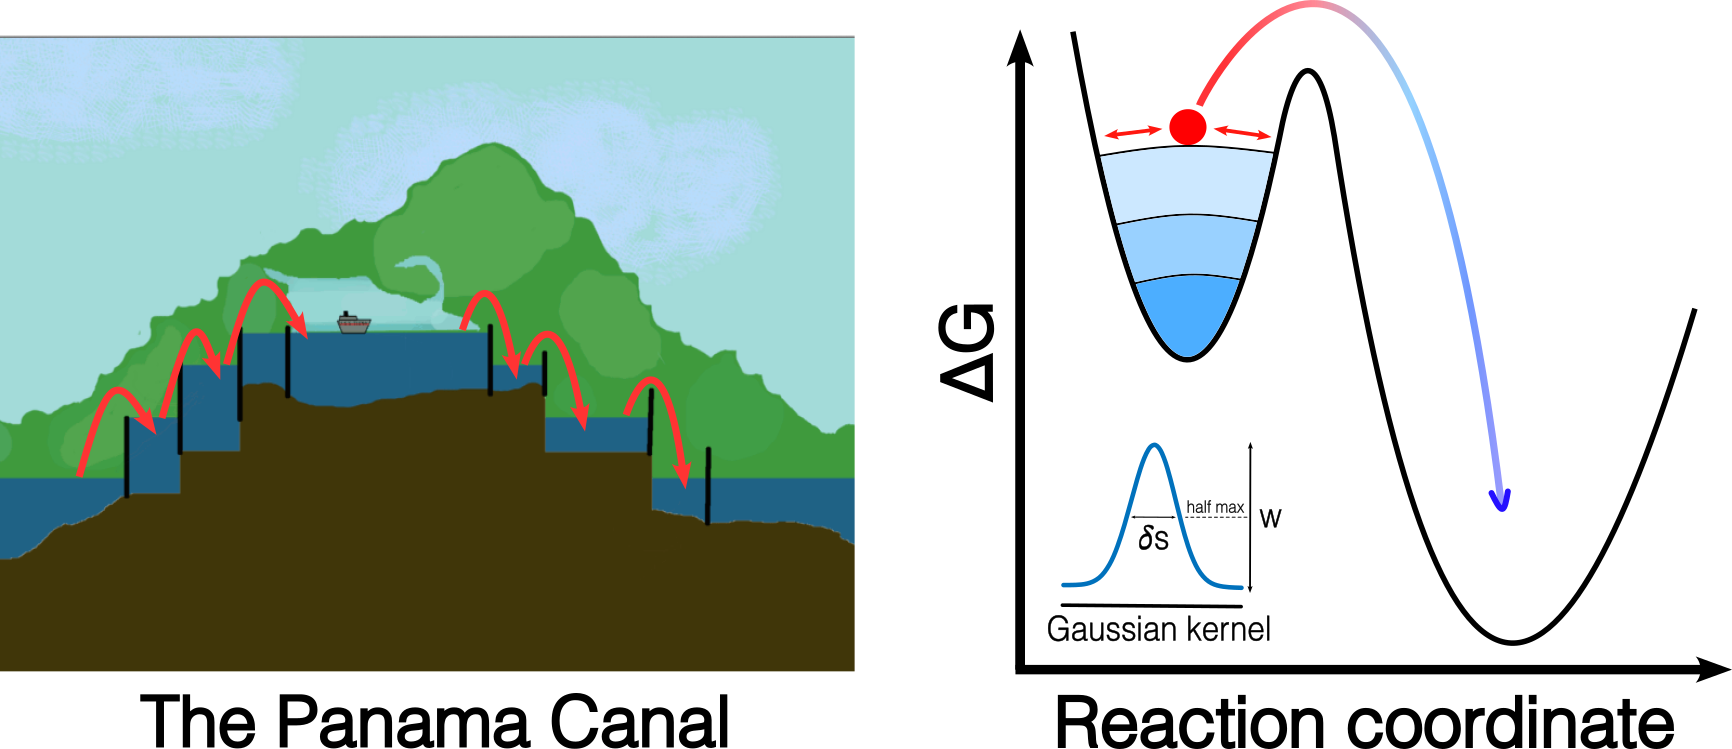
\includegraphics[width=0.8\textwidth]{Figures/2_Theory/theory_metadynamics.png}
    \caption{The concept of metadynamics. $w$ stands for the Gaussian kernel height, and $\delta s$ stands for its width. The Panama Canal cartoon was taken from~\citep{HowPanamaCanal}.}
    \label{fig:metadynamics}
\end{figure}

\begin{equation}
    \dot{V}(s,t) = \frac{\omega \Delta T \delta_{s,s(t)}}{\Delta T + \omega N(s,t)} 
    = \omega e^{-[V(s,t)/\Delta T]} \delta_{s,s(t)}
    \label{eq:hill_deposition_rate}
\end{equation}

The height of the Gaussian kernels used is:

\begin{equation}
    w = \omega e^{-[V(s,t)/\Delta T]} \tau_{\text{G}}
    \label{eq:hill_height}
\end{equation}

where $\tau_{\text{G}}$ is the deposition rate and $\omega$ represents the initial bias deposition rate. The Gaussian kernel height is now dependent on the history of the system, allowing for a more controlled exploration of the free energy landscape.

Ultimately, the underlying free energy surface can be estimated using the following equation:

\begin{equation}
    \tilde{F}(s,t) = -\frac{T + \Delta T}{\Delta T} V(s,t) 
    = -(T + \Delta T) \ln\left(1 + \frac{\omega N(s,t)}{\Delta T} \right)
    \label{eq:free_energy_surface_reconstruction}
\end{equation}

The advantage of \ac{wtmd} is that it enables more efficient exploration of the free energy landscape, as the biasing potential adapts according to the trajectory's history. Moreover, the convergence can be easily monitored by observing the decay of the Gaussian height, which should approach zero as the system fully explores the relevant phase space.



%%%%%%%%%%%%%%%%%%%%%%%%%%%%%%%%%%%%%%%%%%%%%%%%%%%%%%%%%%%%%%%%%%%%%%%%%%%%%%%%

% \section{Transition state theory}



%%%%%%%%%%%%%%%%%%%%%%%%%%%%%%%%%%%%%%%%%%%%%%%%%%%%%%%%%%%%%%%%%%%%%%%%%%%%%%%%

\section{The density functional theory tourist}
The discussion in this section is primarily based on the ``Introduction to Computational Chemistry'' textbook written by Jensen~\citep{jensenIntroductionComputationalChemistry2017}, ``Density Functional Theory: a Practical Introduction'' by Scholl and Steckel~\citep{shollDensityFunctionalTheory2011}, and ``A Chemist's Guide to Density Functional Theory'' by Koch and Holthausen~\citep{kochChemistsGuideDensity2015} unless stated otherwise.

\subsection{The Kohn-Sham approach}
In order to describe reactive events in relatively large systems, up to approximately 1,000 atoms, it is necessary to use methods that offer a good balance between accuracy and computational cost. One such method is \ac{dft}, which is based on the Hohenberg-Kohn theorems and the Kohn-Sham equations.

The central idea behind \ac{dft}, established by Hohenberg and Kohn, is that the ground state energy of a many-electron system can be expressed as a functional of the electron density. This reformulation reduces the problem from solving a 3$N$-dimensional wavefunction to working with a 3-dimensional electron density.

The energy functional can be written as:

\begin{equation}
    \begin{aligned}
    E[\rho(\mathbf{r})] &= T_{\text{s}}[\rho] + J[\rho] + E_{\text{Ne}}[\rho] + E_{\text{XC}}[\rho] =  \\
    &= -\frac{1}{2} \sum_{i}^{N} \langle \phi_i | \nabla^2 | \phi_i \rangle \\
    &\quad + \frac{1}{2} \sum_{i}^{N} \sum_{j}^{N} \iint \left| \phi_i(\mathbf{r}_1) \right|^2 \frac{1}{r_{12}} \left| \phi_j(\mathbf{r}_2) \right|^2 d\mathbf{r}_1 d\mathbf{r}_2 \\
    &\quad - \sum_{i}^{N} \sum_{A}^{M} \int \frac{Z_A}{r_{1A}} \left| \phi_i(\mathbf{r}_1) \right|^2 d\mathbf{r}_1 \\
    &\quad + E_{\text{XC}}[\rho(\mathbf{r})] 
    \label{eq:ks_energy}
    \end{aligned}
\end{equation}

Here, the first three terms are “known” and represent the kinetic energy of the electrons, the Coulomb interaction between the electrons, and the electron-nucleus interaction, respectively. The final term, the exchange-correlation energy functional, is the unknown component. It contains all the effects that are not straightforward to treat exactly, for instance, the residual part of the kinetic energy and the non-classical electron-electron interactions:

\begin{equation}
    E_{\text{XC}}[\rho] \equiv (T[\rho] - T_{\text{s}}[\rho]) + (E_{\text{ee}}[\rho] - J[\rho])
    \label{eq:xc_energy}
\end{equation}

The biggest challenge in \ac{dft} lies in the formulation of $E_{\text{XC}}$. This term is particularly important, as finding the minimum of the total energy functional, as expressed in Equation~\ref{eq:ks_energy}, depends on its accurate representation.

To address this, the Kohn-Sham approach introduces a set of single-electron equations that can be solved iteratively to obtain the electron density and the total energy of the system. The Kohn-Sham equations are given by:

\begin{equation}
    \left( -\frac{1}{2} \nabla^2 + V_{\text{eff}}(\mathbf{r}) \right) \phi_i = \varepsilon_i \phi_i
    \label{eq:ks_equations}
\end{equation}

Here, $V_{\text{eff}}$ takes the form:

\begin{equation}
    V_{\text{eff}}(\mathbf{r}) = \int \frac{\rho(\mathbf{r}_2)}{r_{12}} d\mathbf{r}_2 + V_{\text{XC}}(\mathbf{r}) - \sum_{A}^{M} \frac{Z_A}{r_{1A}}
    \label{eq:v_eff}
\end{equation}

The iterative procedure to solve these equations proceeds as follows: first, a trial electron density is defined. Then, the Kohn-Sham equations are solved using this trial density to obtain the single-particle wavefunctions. Next, a new electron density is calculated from the obtained wavefunctions. Finally, the new density is compared with the initial trial density. If the two densities match within a given convergence criterion, the ground state electron density has been found, and the total energy of the system can be computed.



\subsection{Generalised gradient approximation and PBE functional}
The field of \ac{dft} has opened new avenues for computational chemists and physicists, enabling them to study the properties of materials and molecules, as well as to investigate the reaction pathways of chemical processes. However, the accuracy of \ac{dft} calculations is highly dependent on the choice of the exchange-correlation functional.

In this work, we focus on the \ac{gga} exchange-correlation functionals, which are widely used in \ac{dft} calculations and are known to provide results close to chemical accuracy at a relatively low computational cost, as can be seen in Figure~\ref{fig:jacobs_ladder}. In fact, the development of \ac{gga} functionals marked a turning point in the acceptance of the \ac{dft} method by the quantum chemistry community.

The \ac{gga} functionals are based on the idea that the exchange-correlation energy can be expressed as a functional of the electron density $\rho$ and its gradient $\nabla \rho$. The general form of a \ac{gga} functional is given by:

\begin{equation}
E_{\text{XC}}^{\text{GGA}}[\rho] = \int f(\rho, \nabla\rho) \, d\mathbf{r}
\label{eq:gga_functional}
\end{equation}

The exchange-correlation energy can be explicitly divided into two parts:

\begin{equation}
E_{\text{XC}}^{\text{GGA}} = E_{\text{X}}^{\text{GGA}} + E_{\text{C}}^{\text{GGA}}
\label{eq:gga_xc}
\end{equation}

One of the most widely used \ac{gga} functionals is the Perdew-Burke-Ernzerhof (PBE) functional~\citep{perdewGeneralizedGradientApproximation1996}. Its formulation incorporates parameters in the exchange and correlation parts derived from first principles, making it a truly \textit{ab initio} functional.

\begin{figure}[b!]
    \centering
    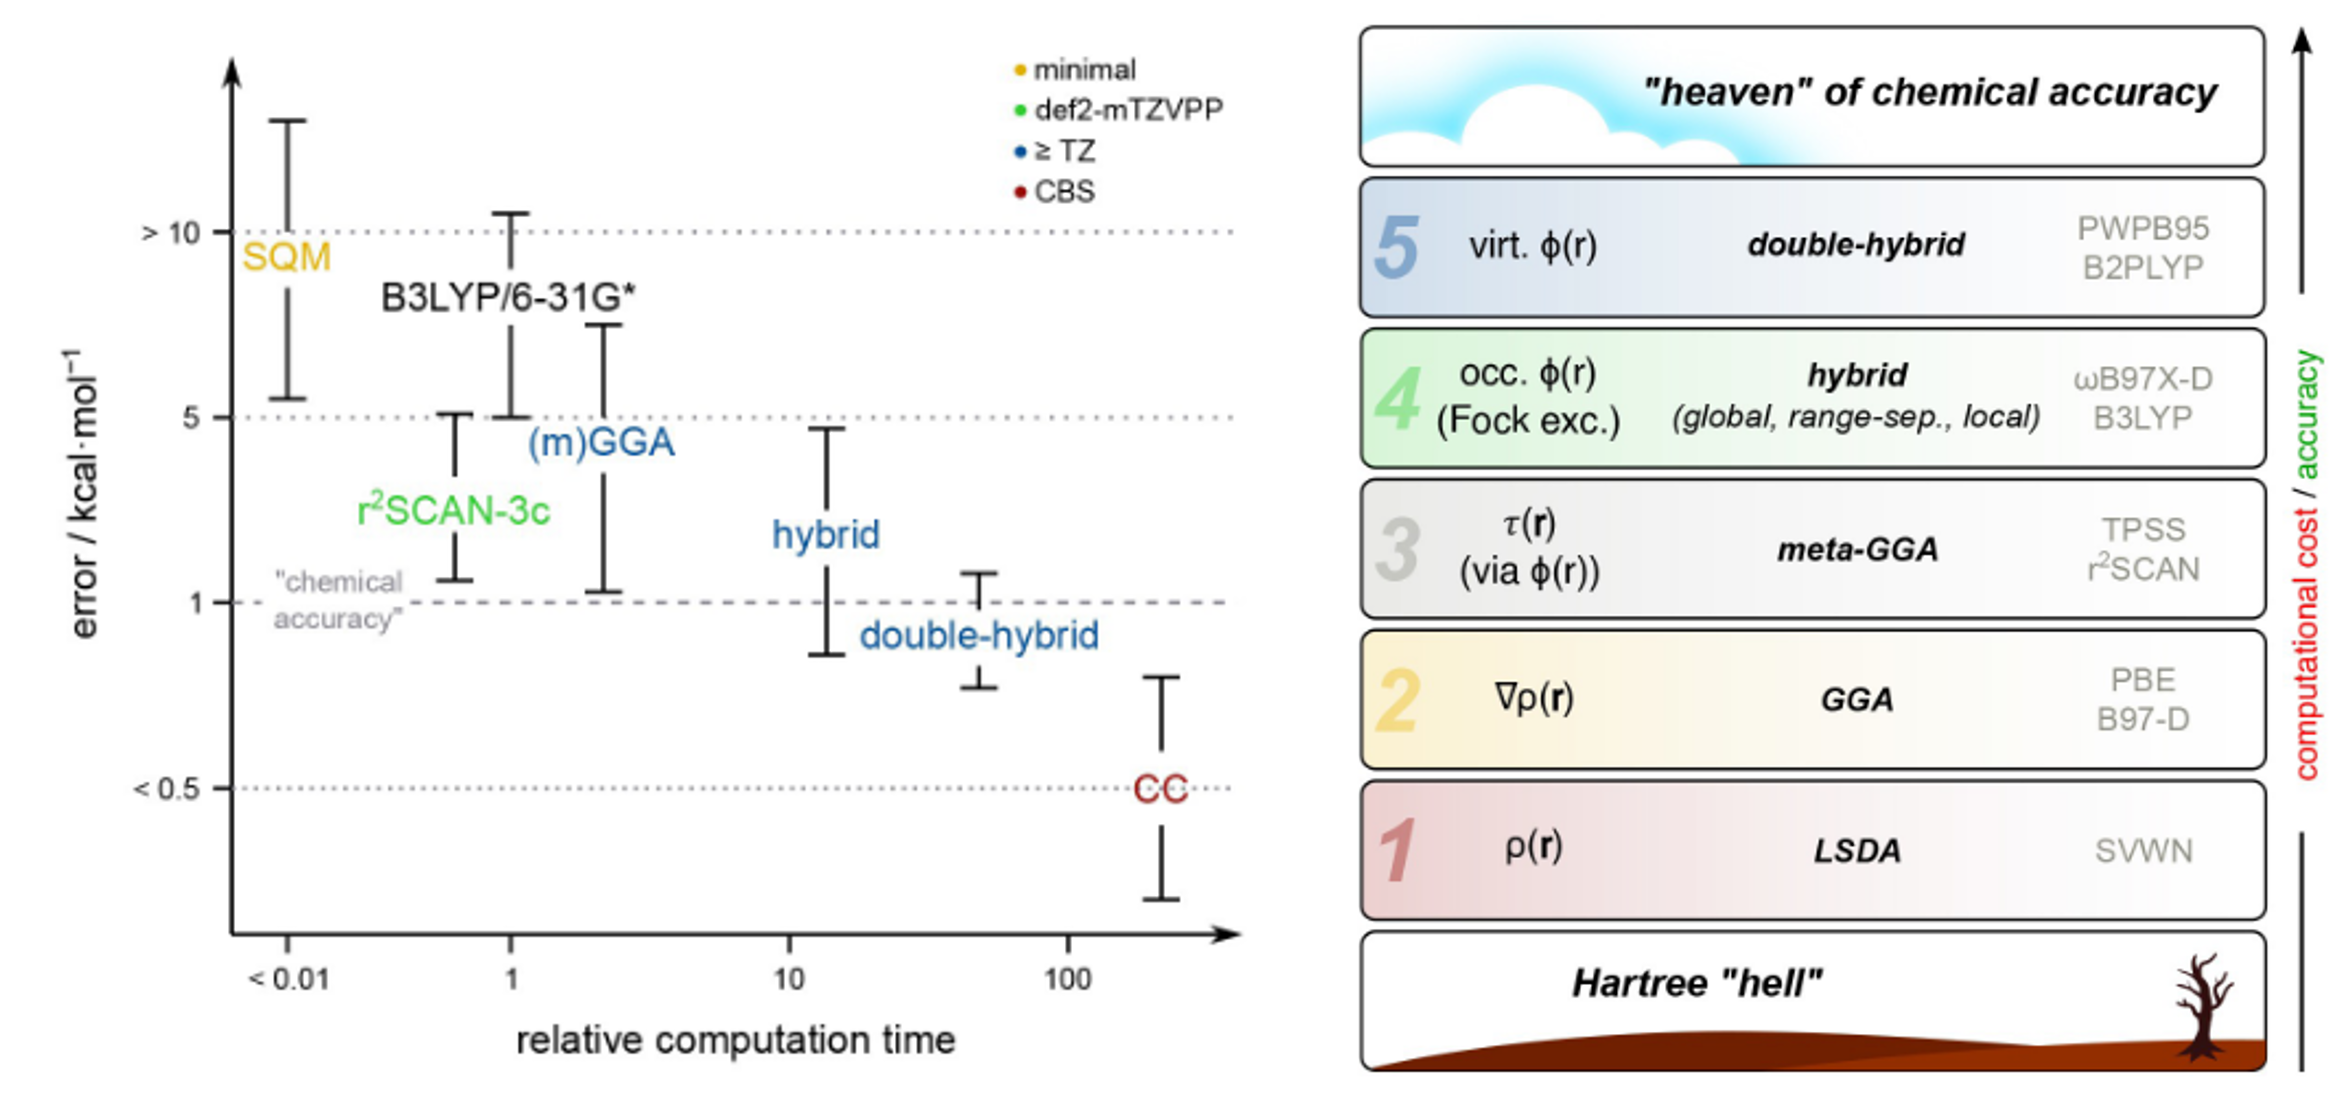
\includegraphics[width=0.7\textwidth]{Figures/2_Theory/theory_jacobs_ladder.png}
    \caption{Left panel: accuracy of the common quantum chemical methods as a function of the computatinal cost. Right panel: categorisation of the exchange-correlation functionals according to Perdew's ``Jacob's ladder''. The figure was reproduced from \citep{burschBestPracticeDFTProtocols2022}.}
    \label{fig:jacobs_ladder}
\end{figure}



\subsection{\textit{Ab initio} molecular dynamics}
In one of the previous sections, we touched upon the topic of classical \ac{md} simulations. However, classical force fields are unable to simulate bond-breaking and bond-forming processes. Although reactive events can also be studied using static approaches, by calculating the potential energy surface at a given set of coordinates, we believe that incorporating dynamics provides more informative insights and a clearer picture of the reaction mechanism.

To simulate the dynamics of a chemical reaction, one could consider using \ac{aimd}, and in particular, \ac{bomd}. In \ac{bomd}, the forces acting on the atoms are calculated at each time step using quantum mechanical methods, such as \ac{dft}, while the nuclei are propagated according to classical mechanics. This process can be described using the Lagrangian formalism, $L$, which offers an alternative formulation of classical dynamics:

\begin{equation}
    L = K - U = \frac{1}{2} \sum_{i=1}^{3N} m_i v_i^2 - E[\phi(\mathbf{r}_1, \ldots, \mathbf{r}_{3N})]
    \label{eq:lagrangian_aimd}
\end{equation}

where $K$ is the kinetic energy, $U$ represents the potential energy, and $\phi(\mathbf{r}_1, \ldots, \mathbf{r}_{3N})$ is a set of one-electron Kohn-Sham wave functions.

It is important to note that, since nuclear dynamics are treated classically in this framework, zero-point vibrational energy is not accounted for, nor can tunnelling effects be studied. 



%%%%%%%%%%%%%%%%%%%%%%%%%%%%%%%%%%%%%%%%%%%%%%%%%%%%%%%%%%%%%%%%%%%%%%%%%%%%%%%%

\section{Extended tight binding}

\begin{equation}
    E[\rho] = E^{(0)}[\rho_0] + E^{(1)}[\rho_0, \delta \rho] + E^{(2)}[\rho_0, (\delta \rho)^2] + E^{(3)}[\rho_0, (\delta \rho)^3] + \cdots
    \label{eq:tb_energy_expansion}
\end{equation}

\begin{equation}
    \begin{aligned}
    E_{\text{GFN1-xTB}} &= E_{\text{rep}}^{(0)} + E_{\text{disp}}^{(0)} + E_{\text{XB}}^{(0)} + E_{\text{EHT}}^{(1)} + E_{\text{IES+IXC}}^{(2)} + E_{\text{IES+IXC}}^{(3)} \\
    &= E_{\text{rep}} + E_{\text{disp}}^{\text{D3}} + E_{\text{XB}}^{\text{GFN1}} + E_{\text{EHT}} + E_{\gamma} + E_{\Gamma}^{\text{GFN1}}
    \end{aligned}
    \label{eq:gfn1xtb_energy}
\end{equation}




%%%%%%%%%%%%%%%%%%%%%%%%%%%%%%%%%%%%%%%%%%%%%%%%%%%%%%%%%%%%%%%%%%%%%%%%%%%%%%%%
\section{Neural network potentials}

\begin{figure}[t!]
    \centering
    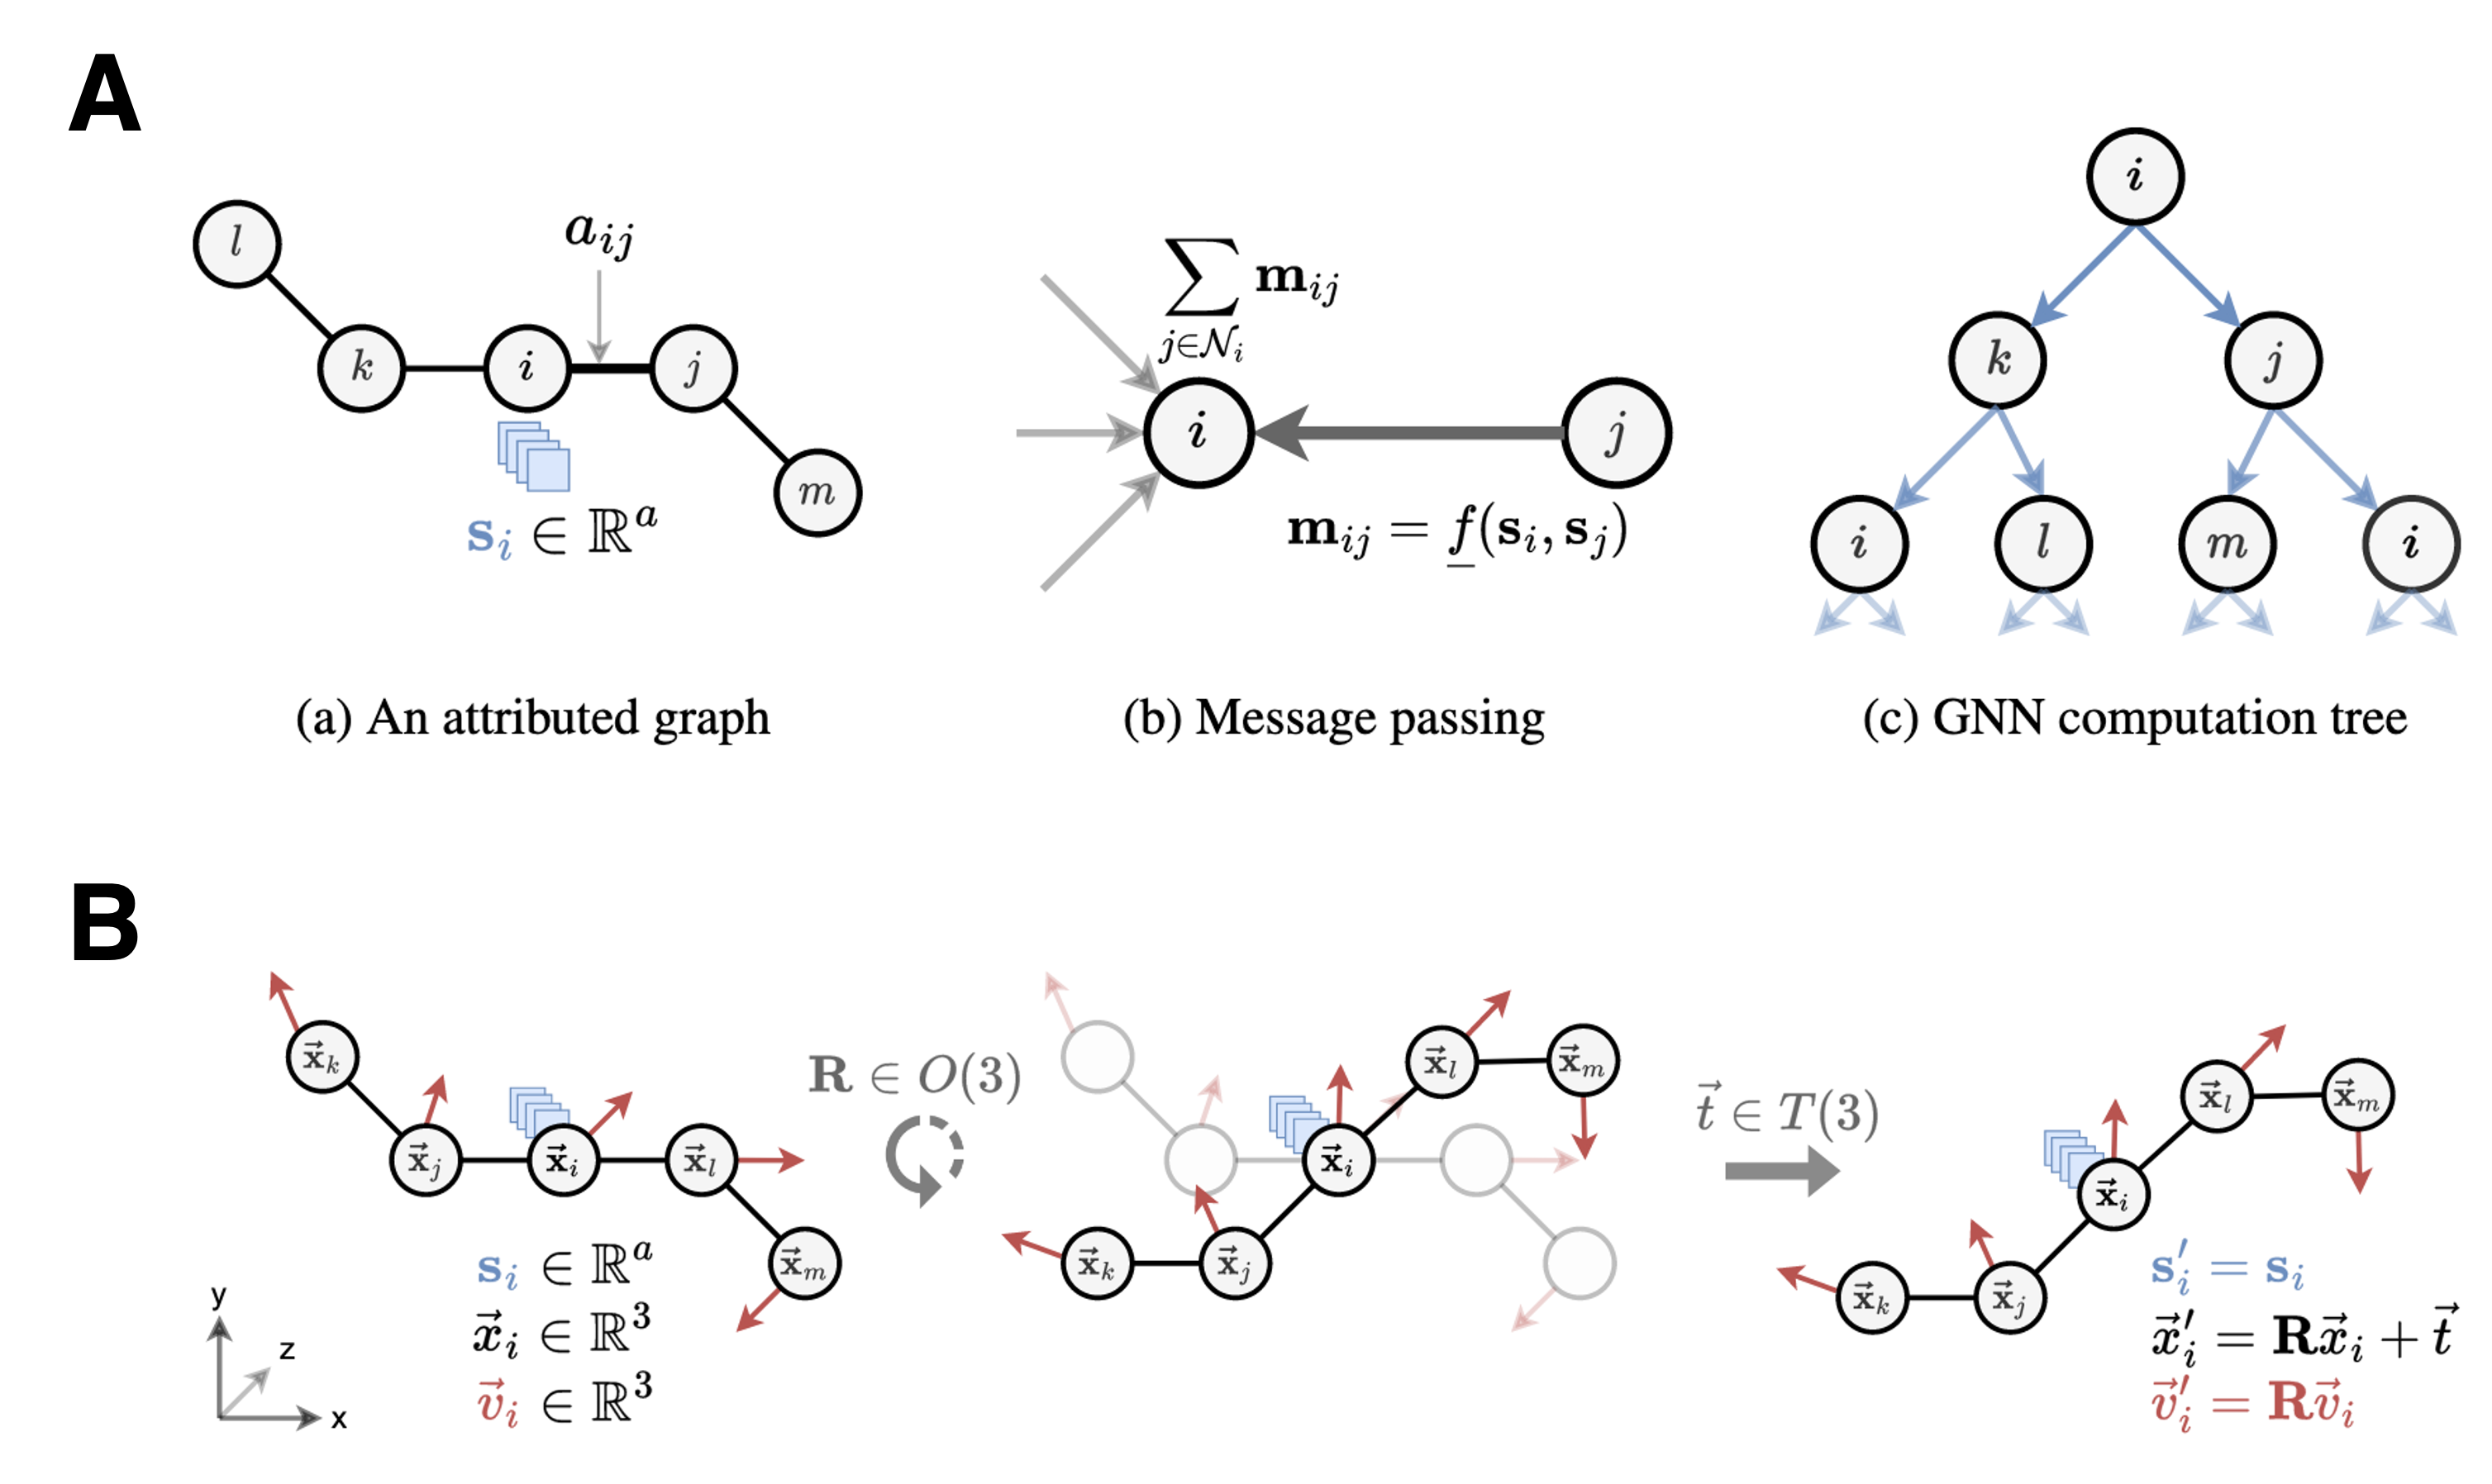
\includegraphics[width=0.7\textwidth]{Figures/2_Theory/graph_and_geometric_nns.png}
    \caption{This figure was reproduced from \citep{duvalHitchhikersGuideGeometric2024}.}
    \label{fig:graph_and_geometric_nns}
\end{figure}

The discussion in this section is mainly based on the textbook ``Deep Learning: Foundations and Concepts'' by C. M. Bishop and H. Bishop~\citep{bishopDeepLearningFoundations2023}, the excellent review by Duval, Mathis, Joshi, and Schmidt et al.~\citep{duvalHitchhikersGuideGeometric2024}, the research paper by Batatia and Batzner et al.~\citep{batatiaDesignSpaceE3Equivariant2022}, and the research paper by Batzner et al.~\citep{batznerE3equivariantGraphNeural2022}, unless stated otherwise.

\subsection{Graph neural networks}
One can easily imagine how computationally expensive it would be to run \ac{aimd} simulations for a system containing hundreds of atoms. In recent years, the field of machine learning has made significant progress in addressing this challenge. In particular, the development of \acp{gnn} has enabled the design of \acp{nnp}, which learn the potential energy surface of molecular systems and can replace \ac{dft} in molecular dynamics simulations.

A natural question one may ask here: why use \acp{gnn}? The answer lies in the fact that \acp{gnn} provide a natural way to represent molecular systems. Atoms can be considered as nodes in a graph, with bonds between them represented as edges. This concept is visualised in Figure~\ref{fig:graph_and_geometric_nns}~A. 

An essential property of any graph $\mathcal{G} = (\mathbf{A}, \mathbf{S})$ is its adjacency matrix $\mathbf{A}$, which encodes the connectivity of the nodes via elements $a_{ij}$. This matrix is square with dimensions $n \times n$, where $n$ is the number of nodes in the graph. Each entry is either 0 or 1, indicating the absence or presence of a connection between two nodes.

Because the ordering of nodes in the graph is arbitrary, \acp{gnn} are, by construction, permutation symmetric.

In addition to the adjacency matrix, each graph also has a matrix of scalar features $\mathbf{S}$ associated with its nodes. In the case of molecular systems, these features may include atomic numbers or atom types.

\Acp{gnn} are neural networks specifically designed to operate on graph-structured data. They learn representations of nodes, edges, or entire graphs by iteratively updating node features based on their neighbours $\mathcal{N}_i$. This iterative process is commonly referred to as message passing, illustrated in Figure~\ref{fig:graph_and_geometric_nns}~A. Conceptually, the process proceeds as follows:
\begin{enumerate}
    \item At iteration $t$, each node $i$ receives messages from its neighbours $\mathcal{N}_i$:
    \begin{equation}
        \mathbf{m}_{ij}^{(t)} = \underline{\text{MSG}}\left(\mathbf{s}_i^{(t)}, \mathbf{s}_j^{(t)}\right)
        \label{eq:message_passing}
    \end{equation}

    \item These messages are aggregated to update the node's features: $\bigoplus_{j \in \mathcal{N}_i} \mathbf{m}_{ij}^{(t)}$.
        
    \item At iteration $t + 1$, the node's representation is updated using the aggregated messages and its current state:
    \begin{equation}
        \mathbf{s}_i^{(t+1)} = \underline{\text{UPD}}\left(\mathbf{s}_i^{(t)}, \bigoplus_{j \in \mathcal{N}_i} \mathbf{m}_{ij}^{(t)}\right)
        \label{eq:representation_update}
    \end{equation}
\end{enumerate}

The $\underline{\text{MSG}}$ and $\underline{\text{UPD}}$ functions form an entire research topic within \acp{gnn}, and are typically implemented as neural networks themselves. The aggregation operator $\bigoplus$ must be permutation-invariant and can take forms such as summation, averaging, etc. After the final iteration, the resulting node representations can be used to predict properties at various levels, whether for the entire graph, such as the total energy of a molecular system, or at the node or edge level.

A particularly important subclass of \acp{gnn} is the geometric \acp{gnn}, which are designed to handle geometric data in Euclidean space. These are depicted in Figure~\ref{fig:graph_and_geometric_nns}~B. Geometric graphs $\mathcal{G} = (\mathbf{A}, \mathbf{S}, \overrightarrow{\mathbf{x}}, \overrightarrow{\mathbf{v}})$ contain additional information such as atomic coordinates $\overrightarrow{x_i}$ and other vector features $\overrightarrow{v_i}$. These vectors may represent quantities such as velocities or forces.

Geometric \acp{gnn} are tailored to work with data that has an inherent geometric structure, such as point clouds. Their key advantage is in handling symmetry operations, i.e. that under rotations and translations of the data, scalar features remain invariant, or the same, while vector features transform appropriately. This property is crucial for accurately capturing the underlying physics of molecular systems.

\subsection{Invariance and equivariance}

In the context of geometric \acp{gnn}, the concepts of invariance and equivariance play a fundamental role in ensuring that models respect the symmetries of the data they are trained on. These properties are especially crucial when working with molecules, where rotations or translations should not change the outcome of the prediction or should change it in a predictable way.

\begin{figure}[t!]
    \centering
    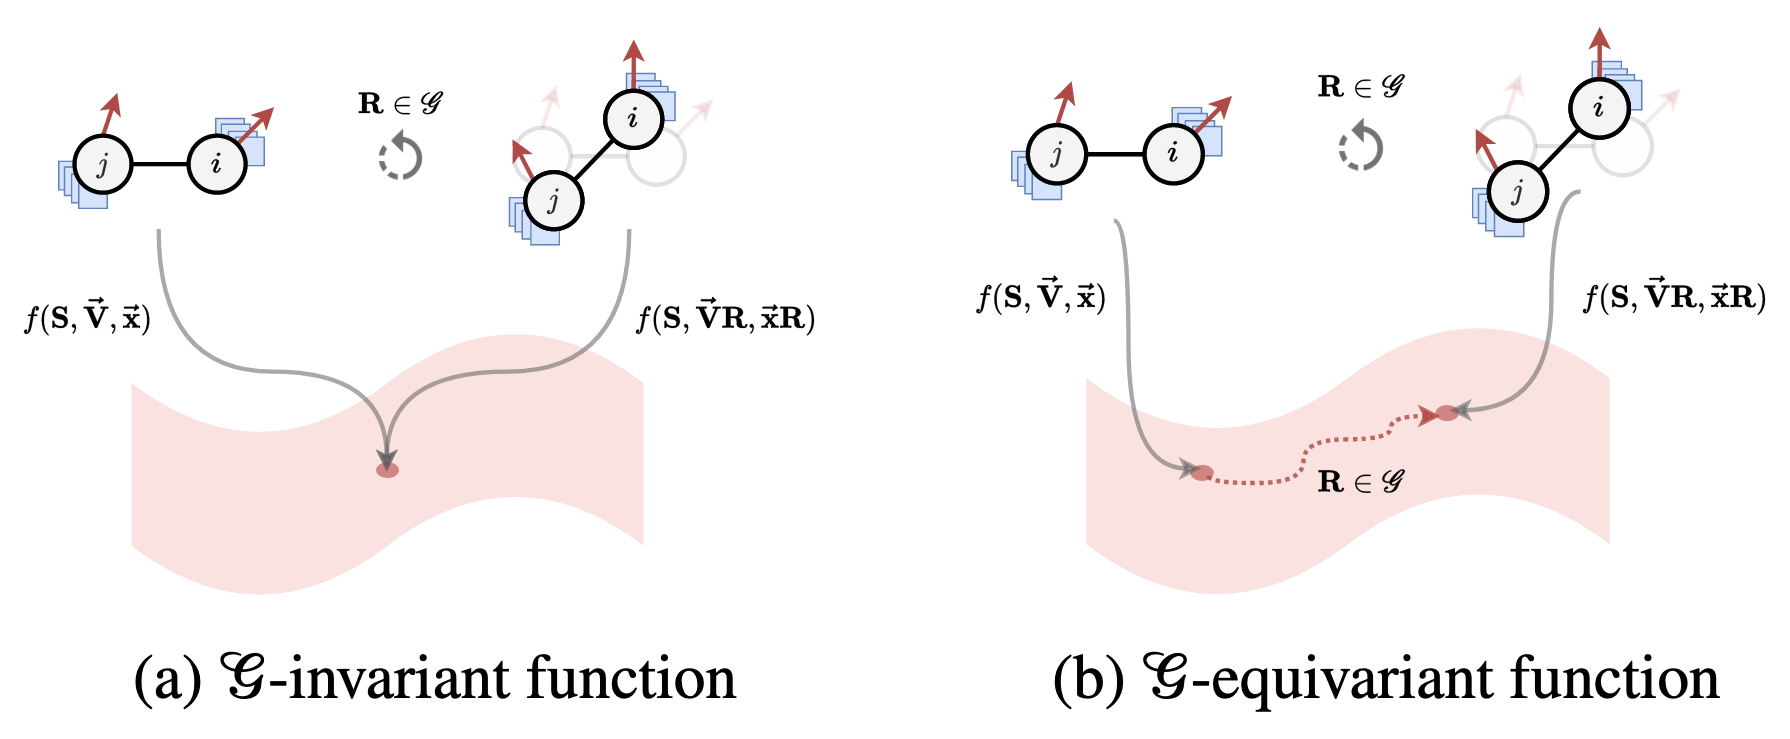
\includegraphics[width=0.8\textwidth]{Figures/2_Theory/invariance_equivariance.png}
    \caption{Invariance and equivariance. This figure was taken from \citep{duvalHitchhikersGuideGeometric2024}.}
    \label{fig:invariance_equivariance}
\end{figure}

Mathematically, a function $f$ is said to be invariant to a transformation $g$ if applying $g$ to the input $x$ does not affect the output of the function:

\begin{equation}
f(g \cdot x) = f(x)
\label{eq:invariance}
\end{equation}

A simple real-world example of invariance is the total energy of a molecule. Typically it stays invariant under rotations and translations of its atomic coordinates.

On the other hand, a function $f$ is said to be equivariant to a transformation $g$ if applying $g$ to the input results in the same transformation being applied to the output:

\begin{equation}
f(g \cdot x) = g \cdot f(x)
\label{eq:equivariance}
\end{equation}

A familiar example of equivariance is the behaviour of vector quantities such as velocity or force. If we rotate a coordinate system (or the object within it), the velocity or force vectors will also rotate accordingly. In the context of molecular systems, atomic forces are equivariant under rotations: if the molecule is rotated, the directions of the forces rotate in the same way. Both concepts of invariance and equivariance are illustrated in Figure~\ref{fig:invariance_equivariance}.

Designing \acp{gnn} that are invariant or equivariant helps reduce the amount of data needed for training. Geometric neural networks, for instance, are explicitly constructed to respect such symmetries, making them particularly well-suited for chemical modelling.

\clearpage
\subsection{Equivariant graph neural networks}

\begin{figure}[b!]
    \centering
    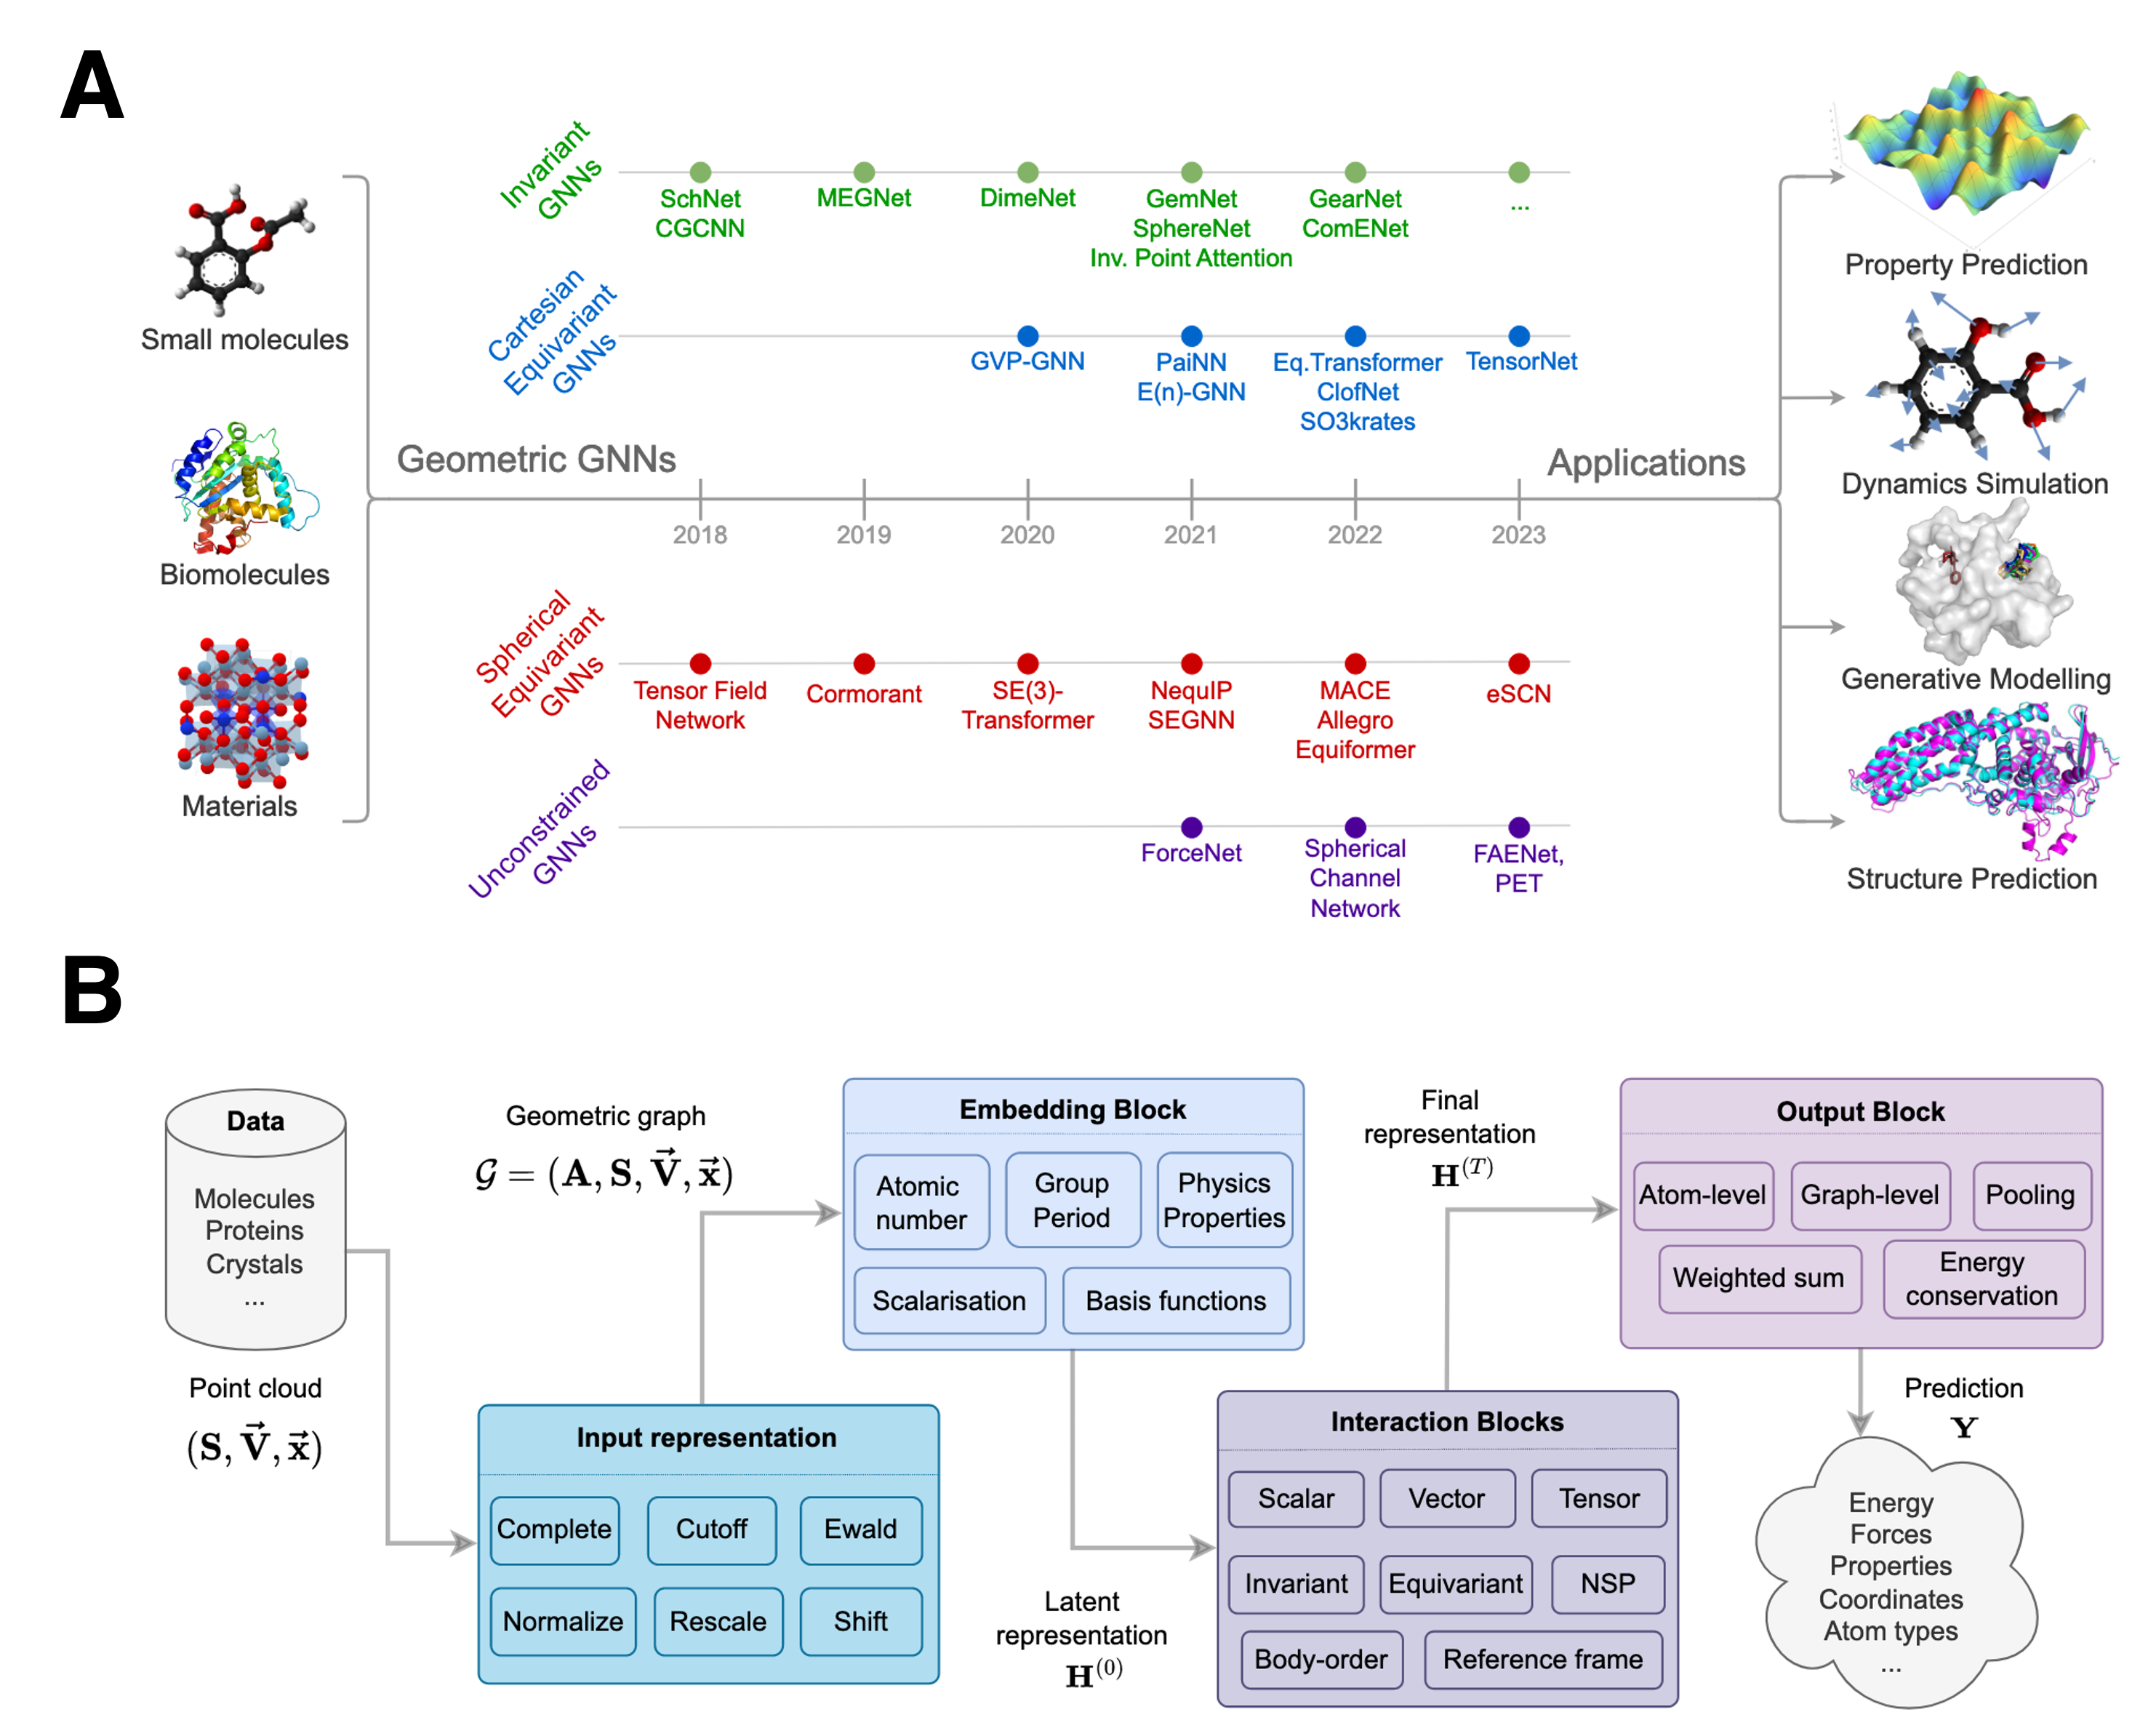
\includegraphics[width=0.7\textwidth]{Figures/2_Theory/equivariant_gnns.png}
    \caption{This figure was reproduced from \citep{duvalHitchhikersGuideGeometric2024}.}
    \label{fig:equivariant_gnns}
\end{figure}
\chapter{Computational Details}
This chapter provides the details of the computational methods used in this work. The first section describes the generation of the training dataset, including the preparation of the system, initial equilibration using the molecular mechanics, exploration of the configuration space at the xTB level, further data labeling, and iterative training of the neural network potential. The second section discusses the production runs at different temperatures using the fitted neural network potential. The third section describes the workflow of validating the transition states obtained from the simulations following the partial Hessian formalism. Finally, the fourth section presents the data analysis and visualisation techniques employed to interpret the results.

\section{Training dataset generation}

\subsection{System preparation}
The systems were prepared using the \texttt{CHARMM-GUI} webserver's functionality \citep{jo_charmm-gui_2008}. In particular, the \texttt{Multicomponent Assembler} interface \citep{kern_charmm-gui_2024} was utilised. 

As a first step, the singly protonated and deprotonated forms of the methyl diphosphate were parametrised in \texttt{CGenFF} \citep{kim_charmm-gui_2017}, i.e. CHARMM General Forcefield. These states of the methyl diphosphate were chosen based on the fact that pyrophosphoric (diphosphoric) acid has the following dissociation constants \citep{haynes_crc_2016}:
\begin{align*}
    \mathrm{H_4P_2O_7} \rightleftharpoons \mathrm{[H_3P_2O_7]^-} + \mathrm{H^+},\quad \mathrm{p}K_\mathrm{a} = 0.91 \\
    \mathrm{[H_3P_2O_7]^-} \rightleftharpoons \mathrm{[H_2P_2O_7]^{2-}} + \mathrm{H^+},\quad \mathrm{p}K_\mathrm{a} = 2.10 \\
    \mathrm{[H_2P_2O_7]^{2-}} \rightleftharpoons \mathrm{[HP_2O_7]^{3-}} + \mathrm{H^+},\quad \mathrm{p}K_\mathrm{a} = 6.70 \\
    \mathrm{[HP_2O_7]^{3-}} \rightleftharpoons \mathrm{[P_2O_7]^{4-}} + \mathrm{H^+},\quad \mathrm{p}K_\mathrm{a} = 9.32
\end{align*}
Thus, at the physiological pH of 7.4 this acid exists as an equillibrium between the doubly and singly protonated forms. As an assumption, the methyl group can be considered as a proton, therefore we condsidered the methyl diphosphate molecule to exist as a mixture of the singly (MeHDP) and deprotonated (MeDP) forms at the physiological pH.

After succesfully parametrising the molecules, the system was solvated in a cubic box of TIP3 water molecules together with the sodium counterions Na\textsuperscript{+} to neutralise the charge. The final system composition can be seen in Table \ref{tab:system-before-equilibration}.

\subsection{Initial equilibration using the classical forcefields}
The equilibration of the system was performed following the standard protocol generated by the \texttt{CHARMM-GUI} webserver \citep{jo_charmm-gui_2008}. The system was first energy minimised using the steepest descent algorithm for 5000 steps. 

Subsequently the system was equillibrated in the NVT (constant number of particles, volume, and temperature) ensemble for 5 ns. During the minimisation and NVT equilibration, the heavy atoms of the solute were restrained using a harmonic potential with a force constant of 400 kJ mol\textsuperscript{-1} nm\textsuperscript{-2}.

As a last step, the system was equilibrated in the NPT (constant number of particles, pressure, and temperature) ensemble for 45 ns. Throughout the whole protocol, the temperature was set to 300 K and the pressure was set to 1 bar. To ensure the constant temperature and pressure, the system was coupled to a $\nu$-rescale thermostat with a coupling constant of 1 ps and an isotropic \textit{c}-rescale barostat with a coupling constant of 5 ps. During the NPT run, the cut-off for the non-bonded interactions was set to 0.6 nm and the long-range electrostatics were treated using the Particle Mesh Ewald (PME) method.

All simulations were conducted in \texttt{GROMACS 2021.4} \citep{abraham_gromacs_2015} using the CHARMM36m forcefield \citep{huang_charmm36m_2017} and the Leap-Frog integration method with a time step of 1 fs. All hydrogen involving bonds were constrained using the LINCS algorithm. The final dimensions of the box for all further calculations were obtained after the NPT run and are shown in Table \ref{tab:system-before-equilibration}.
\begin{table}[htbp]
    \centering
    \caption{System composition and simulation box details. \textsuperscript{1}The final dimensions were obtained after the NPT run using the CHARMM36m forcefield.}
    \label{tab:system-before-equilibration}
    \begin{tabular}{@{}lccc@{}}
    \toprule
    System & Equillibrated box dimensions\textsuperscript{1} (\AA) & No. of water molecules & No. of Na\textsuperscript{+} \\
    \midrule
    MeDP  & $15.877 \times 15.877 \times 15.877$ & 119 & 3 \\
    MeHDP & $15.901 \times 15.901 \times 15.901$ & 124 & 2 \\
    \bottomrule
    \end{tabular}
\end{table}
\subsection{GFN1-xTB based exploration of the configuration space}

\subsection{Data labeling}

\subsection{Iterative training of the neural network potential}

\subsubsection{First round}

\subsubsection{Second round}

\subsubsection{Third round}



\section{Production runs at different temperatures}



\section{Validation of the transition states}



\section{Data analysis and visualisation}
\chapter{Results and discussion}

\section{Final dataset composition}

\begin{figure}[ht]
    \centering
    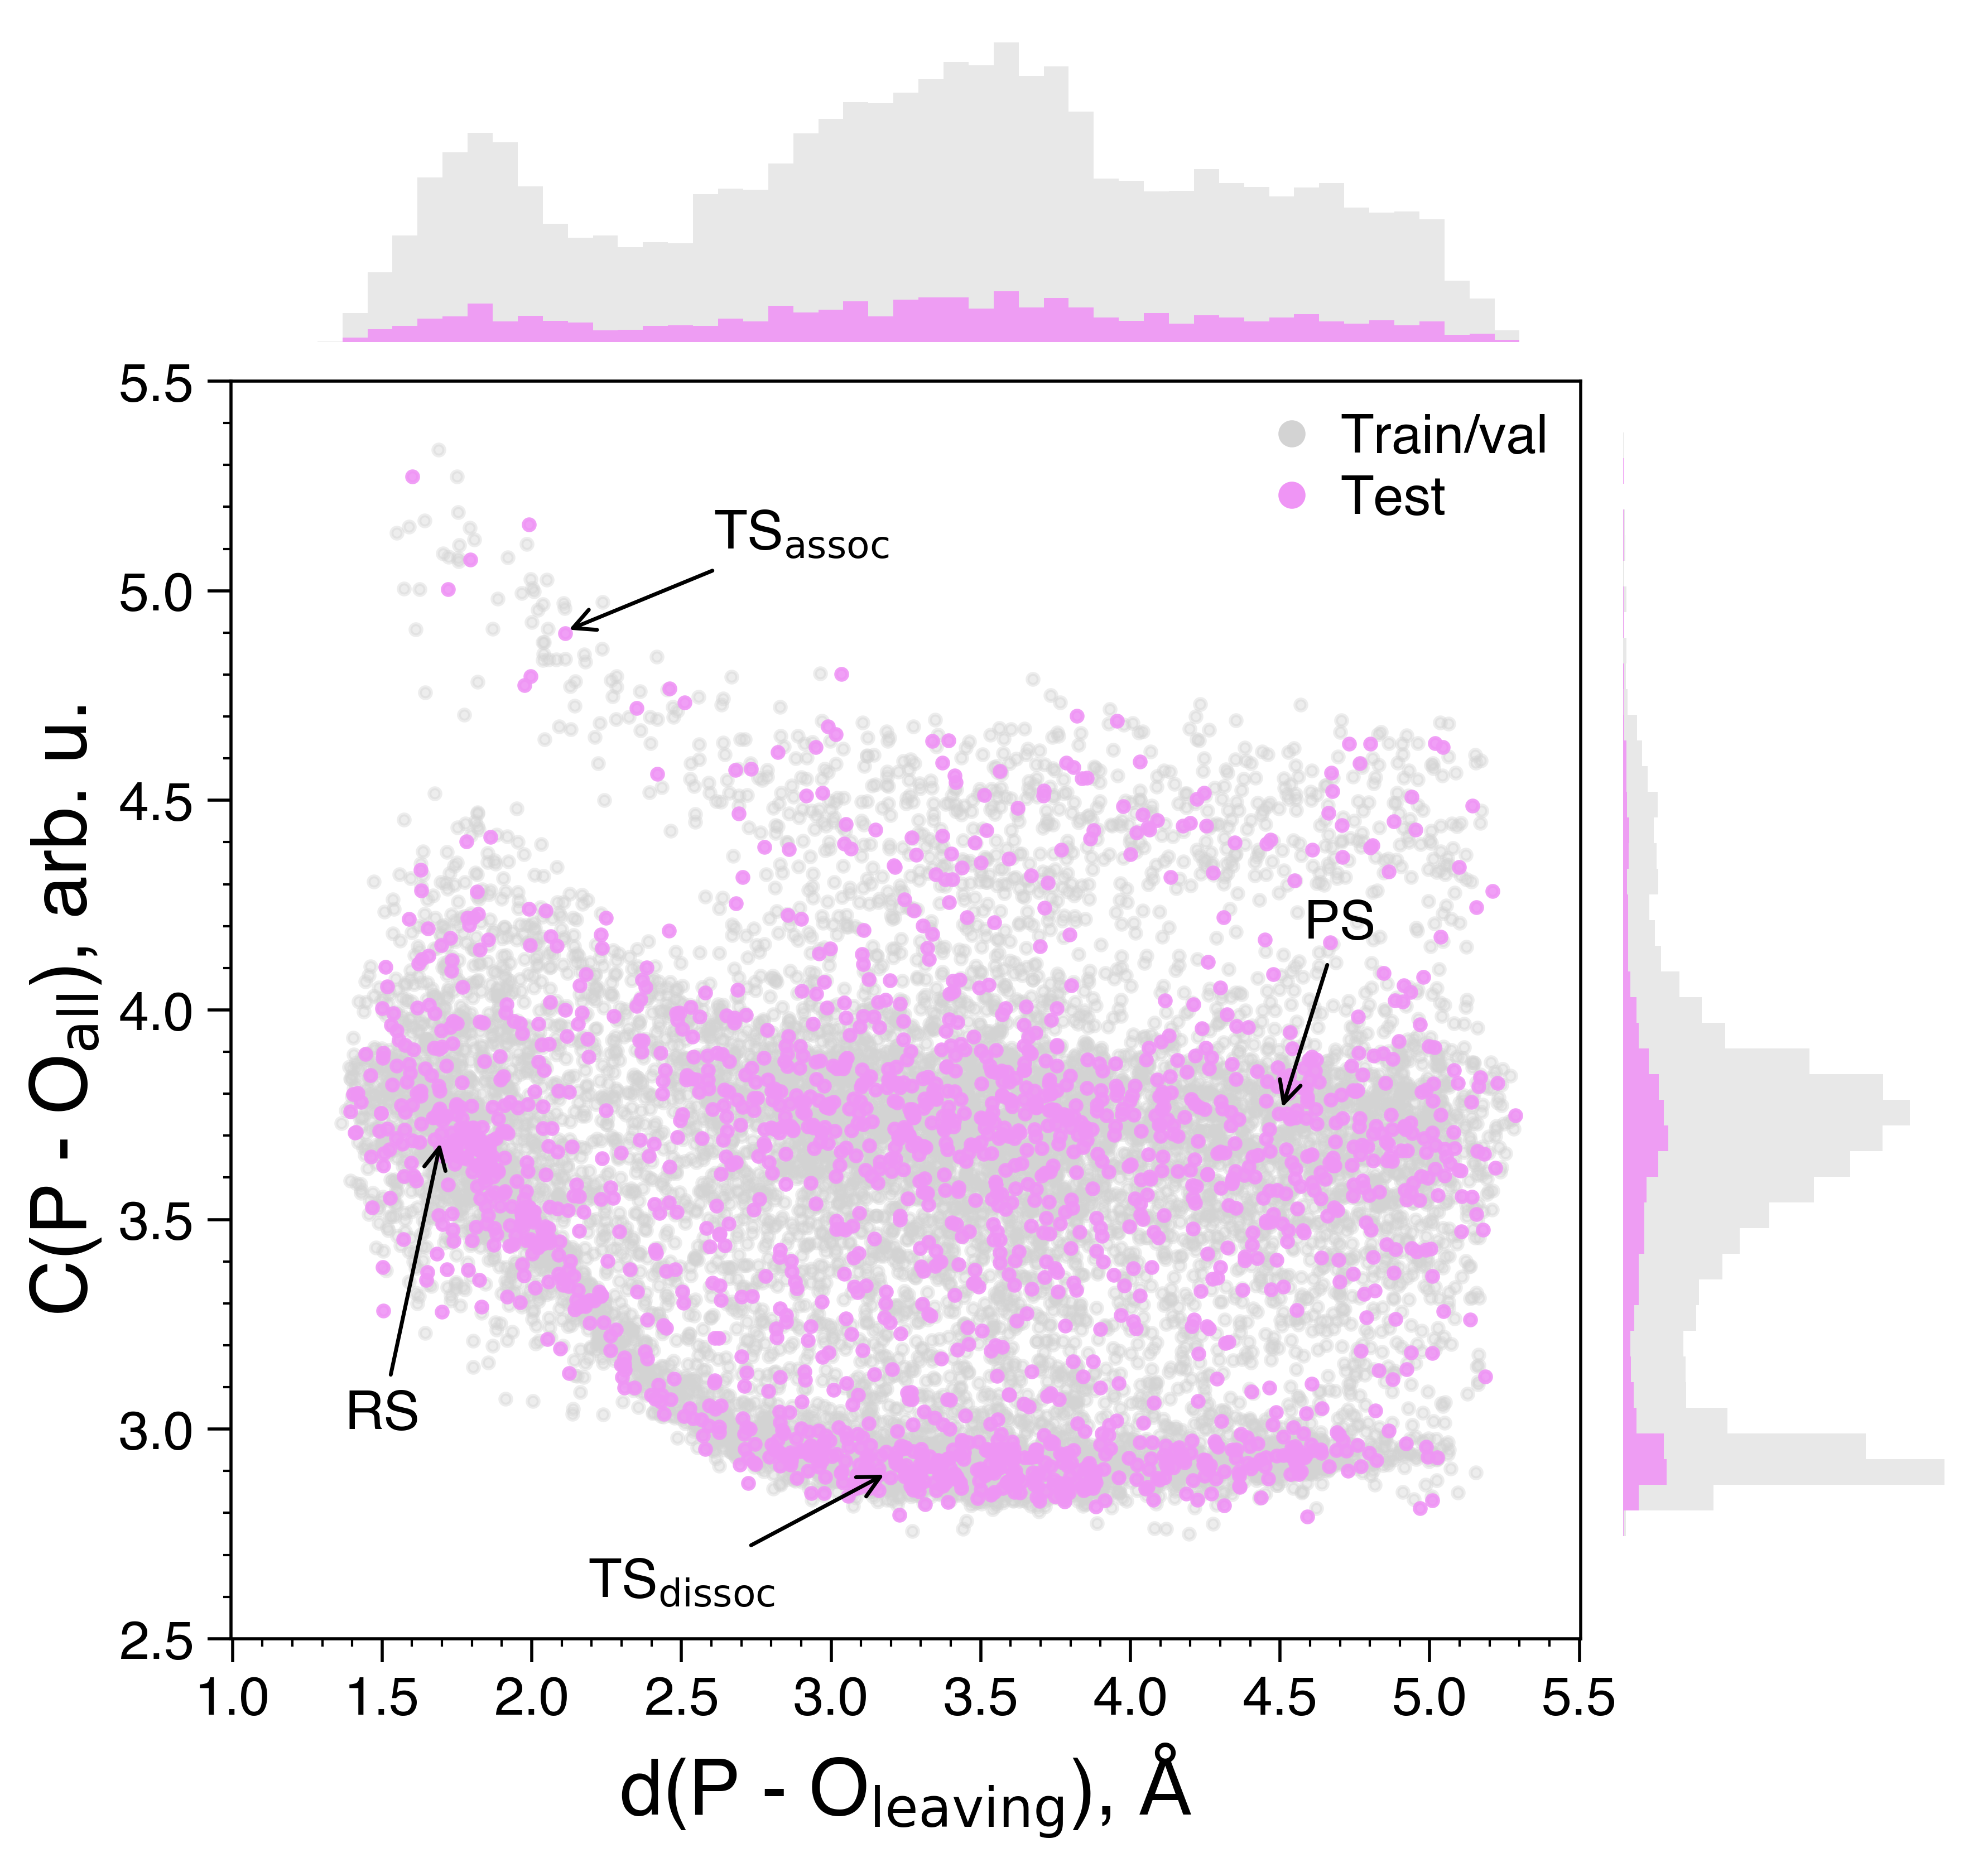
\includegraphics[width=0.9\textwidth]{Figures/4_Results/results_final_dataset_with_histograms.png}
    \caption{Left panel: final dataset composition projected on the two \acp{cv} space. In total, 12,000 data points are visualised for the training and validation parts, as well as 1,800 points for the test set. RS stands for the reactants state, PS for the product state, and TS for the transition state. 50 bins were used to produce the histograms. Right panel: normalised densities of the two \acp{cv} for the training/validation and test sets.}
    \label{fig:final_dataset}
\end{figure}


%%%%%%%%%%%%%%%%%%%%%%%%%%%%%%%%%%%%%%%%%%%%%%%%%%%%%%%%%%%%%%%%%%%%%%%%%%%%%%%%
\clearpage
\section{Accuracy and performance of the neural network potential}

\begin{figure}[ht]
    \centering
    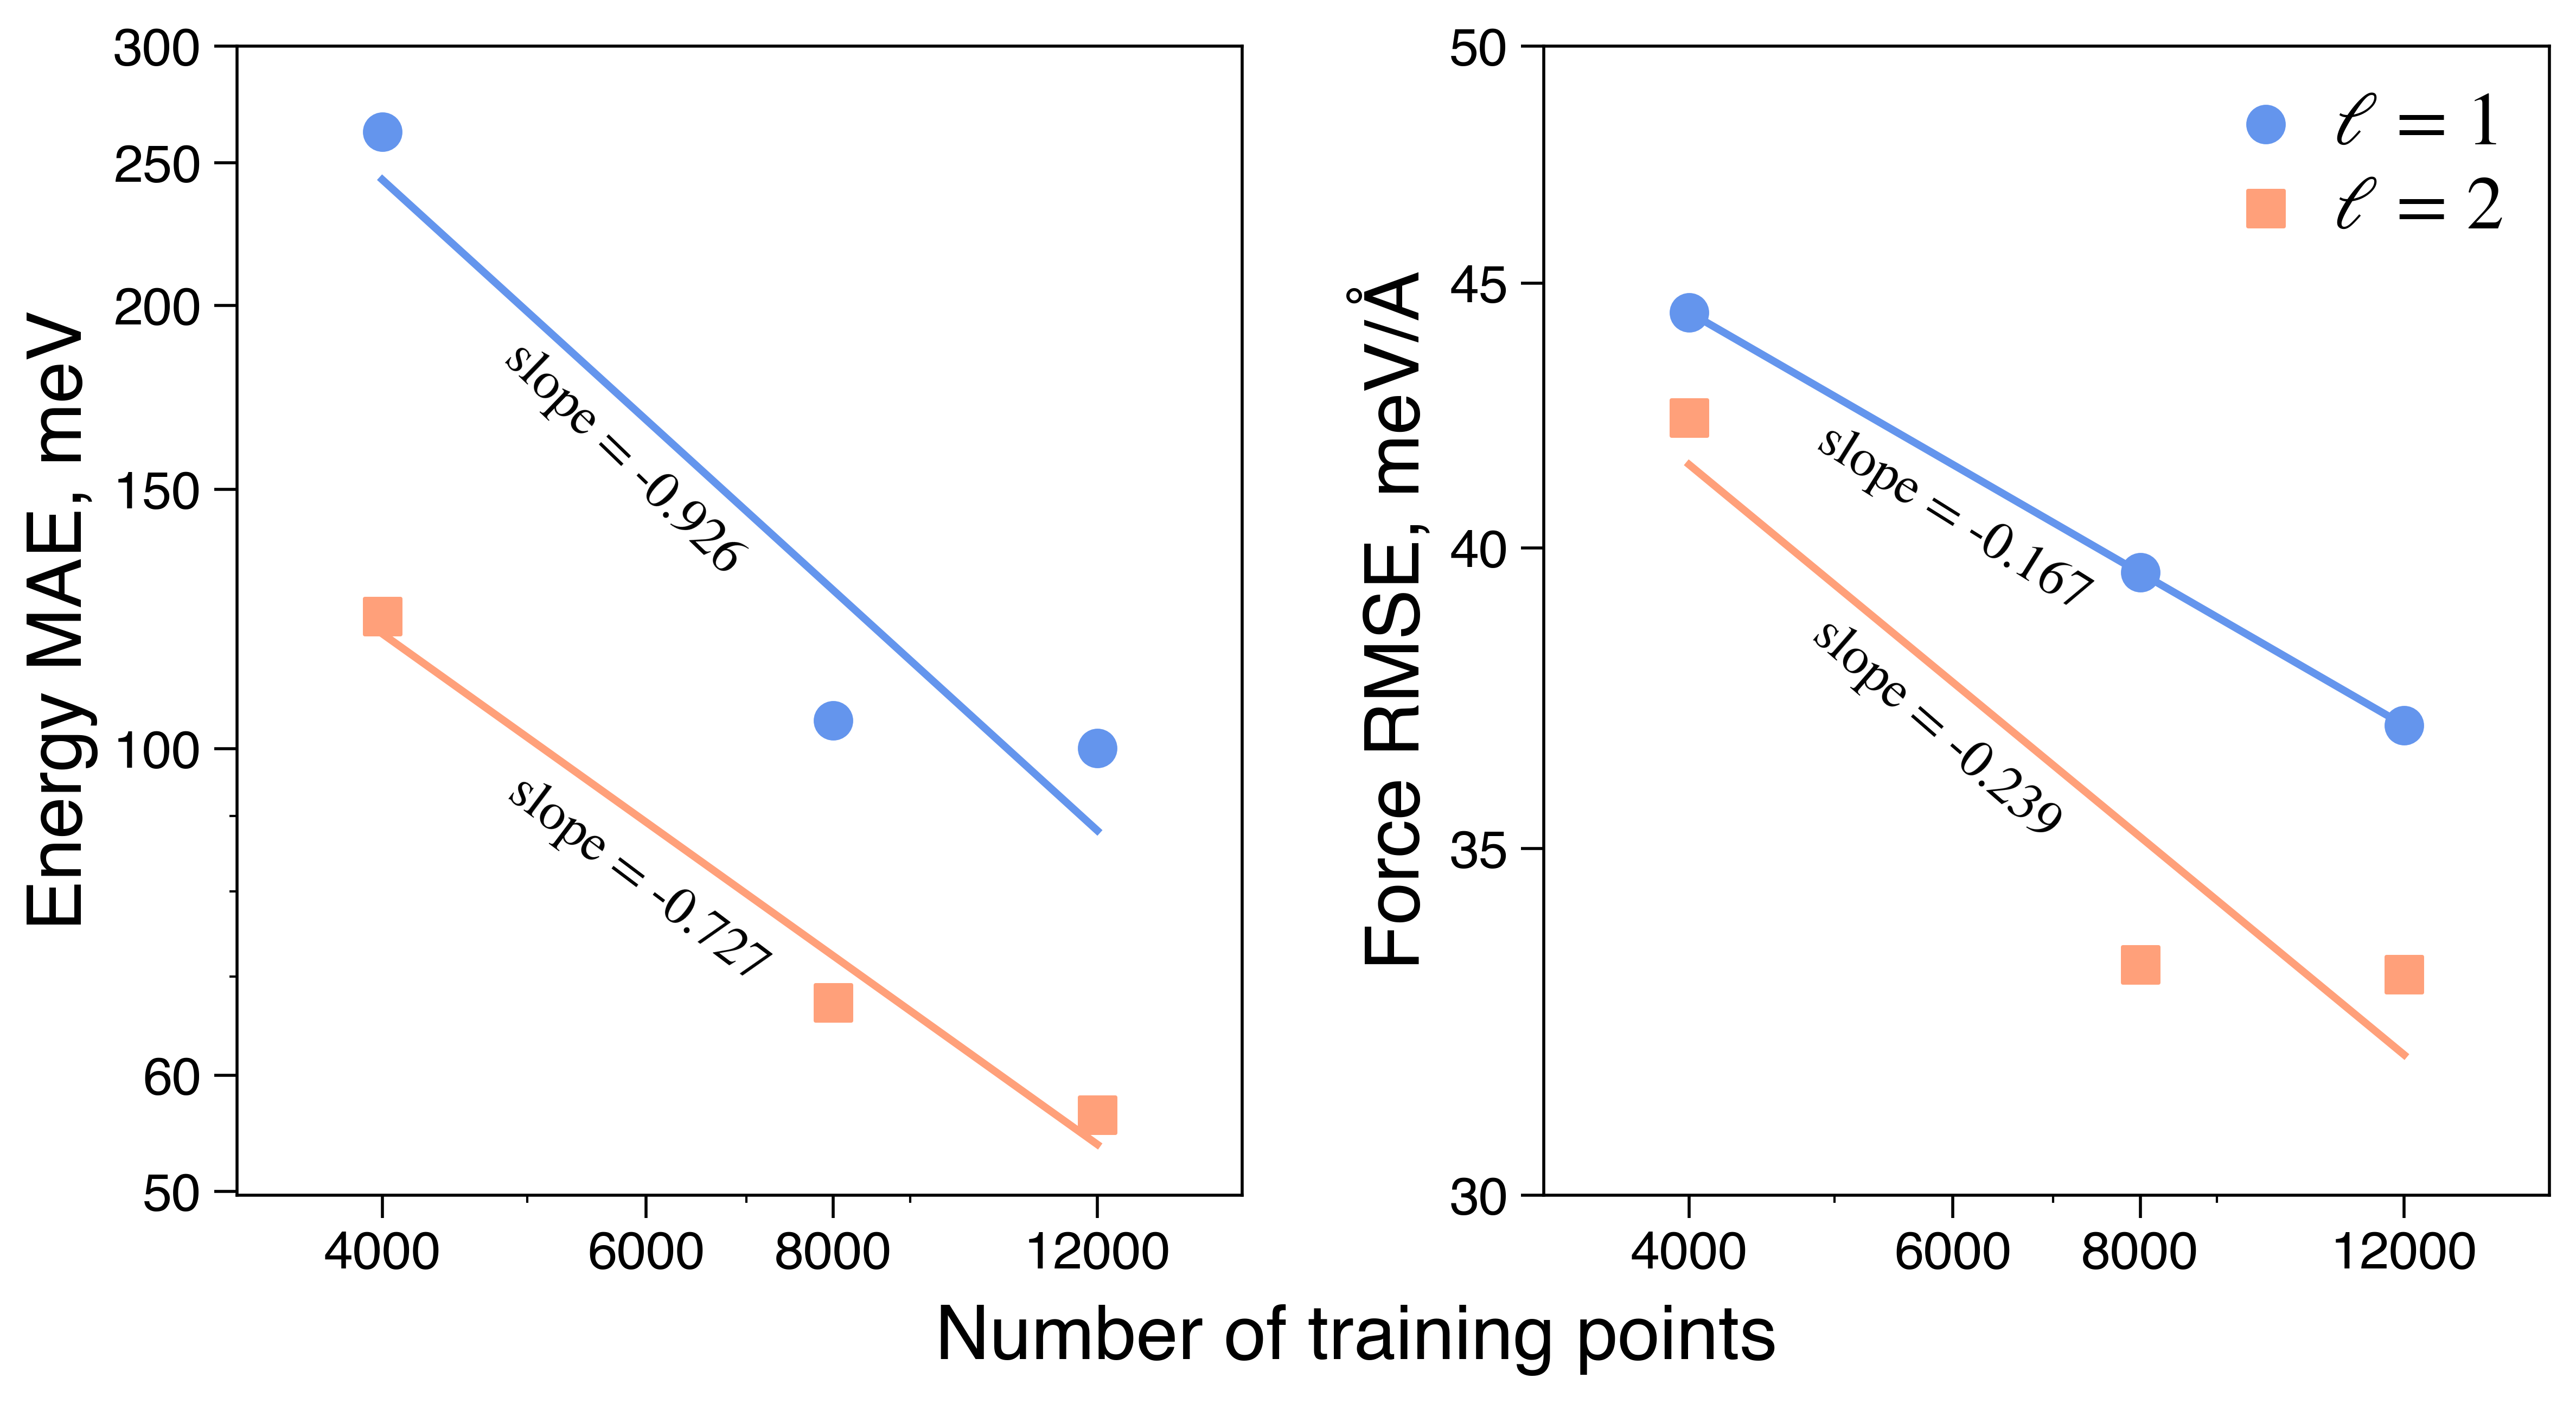
\includegraphics[width=0.8\textwidth]{Figures/4_Results/results_nnp_loglog_energy_force.png}
    \caption{Log-log plot of the errors in the energy and forces for the neural network potential with the respect to the training dataset size. In all cases, the errors were calculated on the final test set of 1,200 data points.}
    \label{fig:nnp_log-log}
\end{figure}

\begin{figure}[ht]
    \centering
    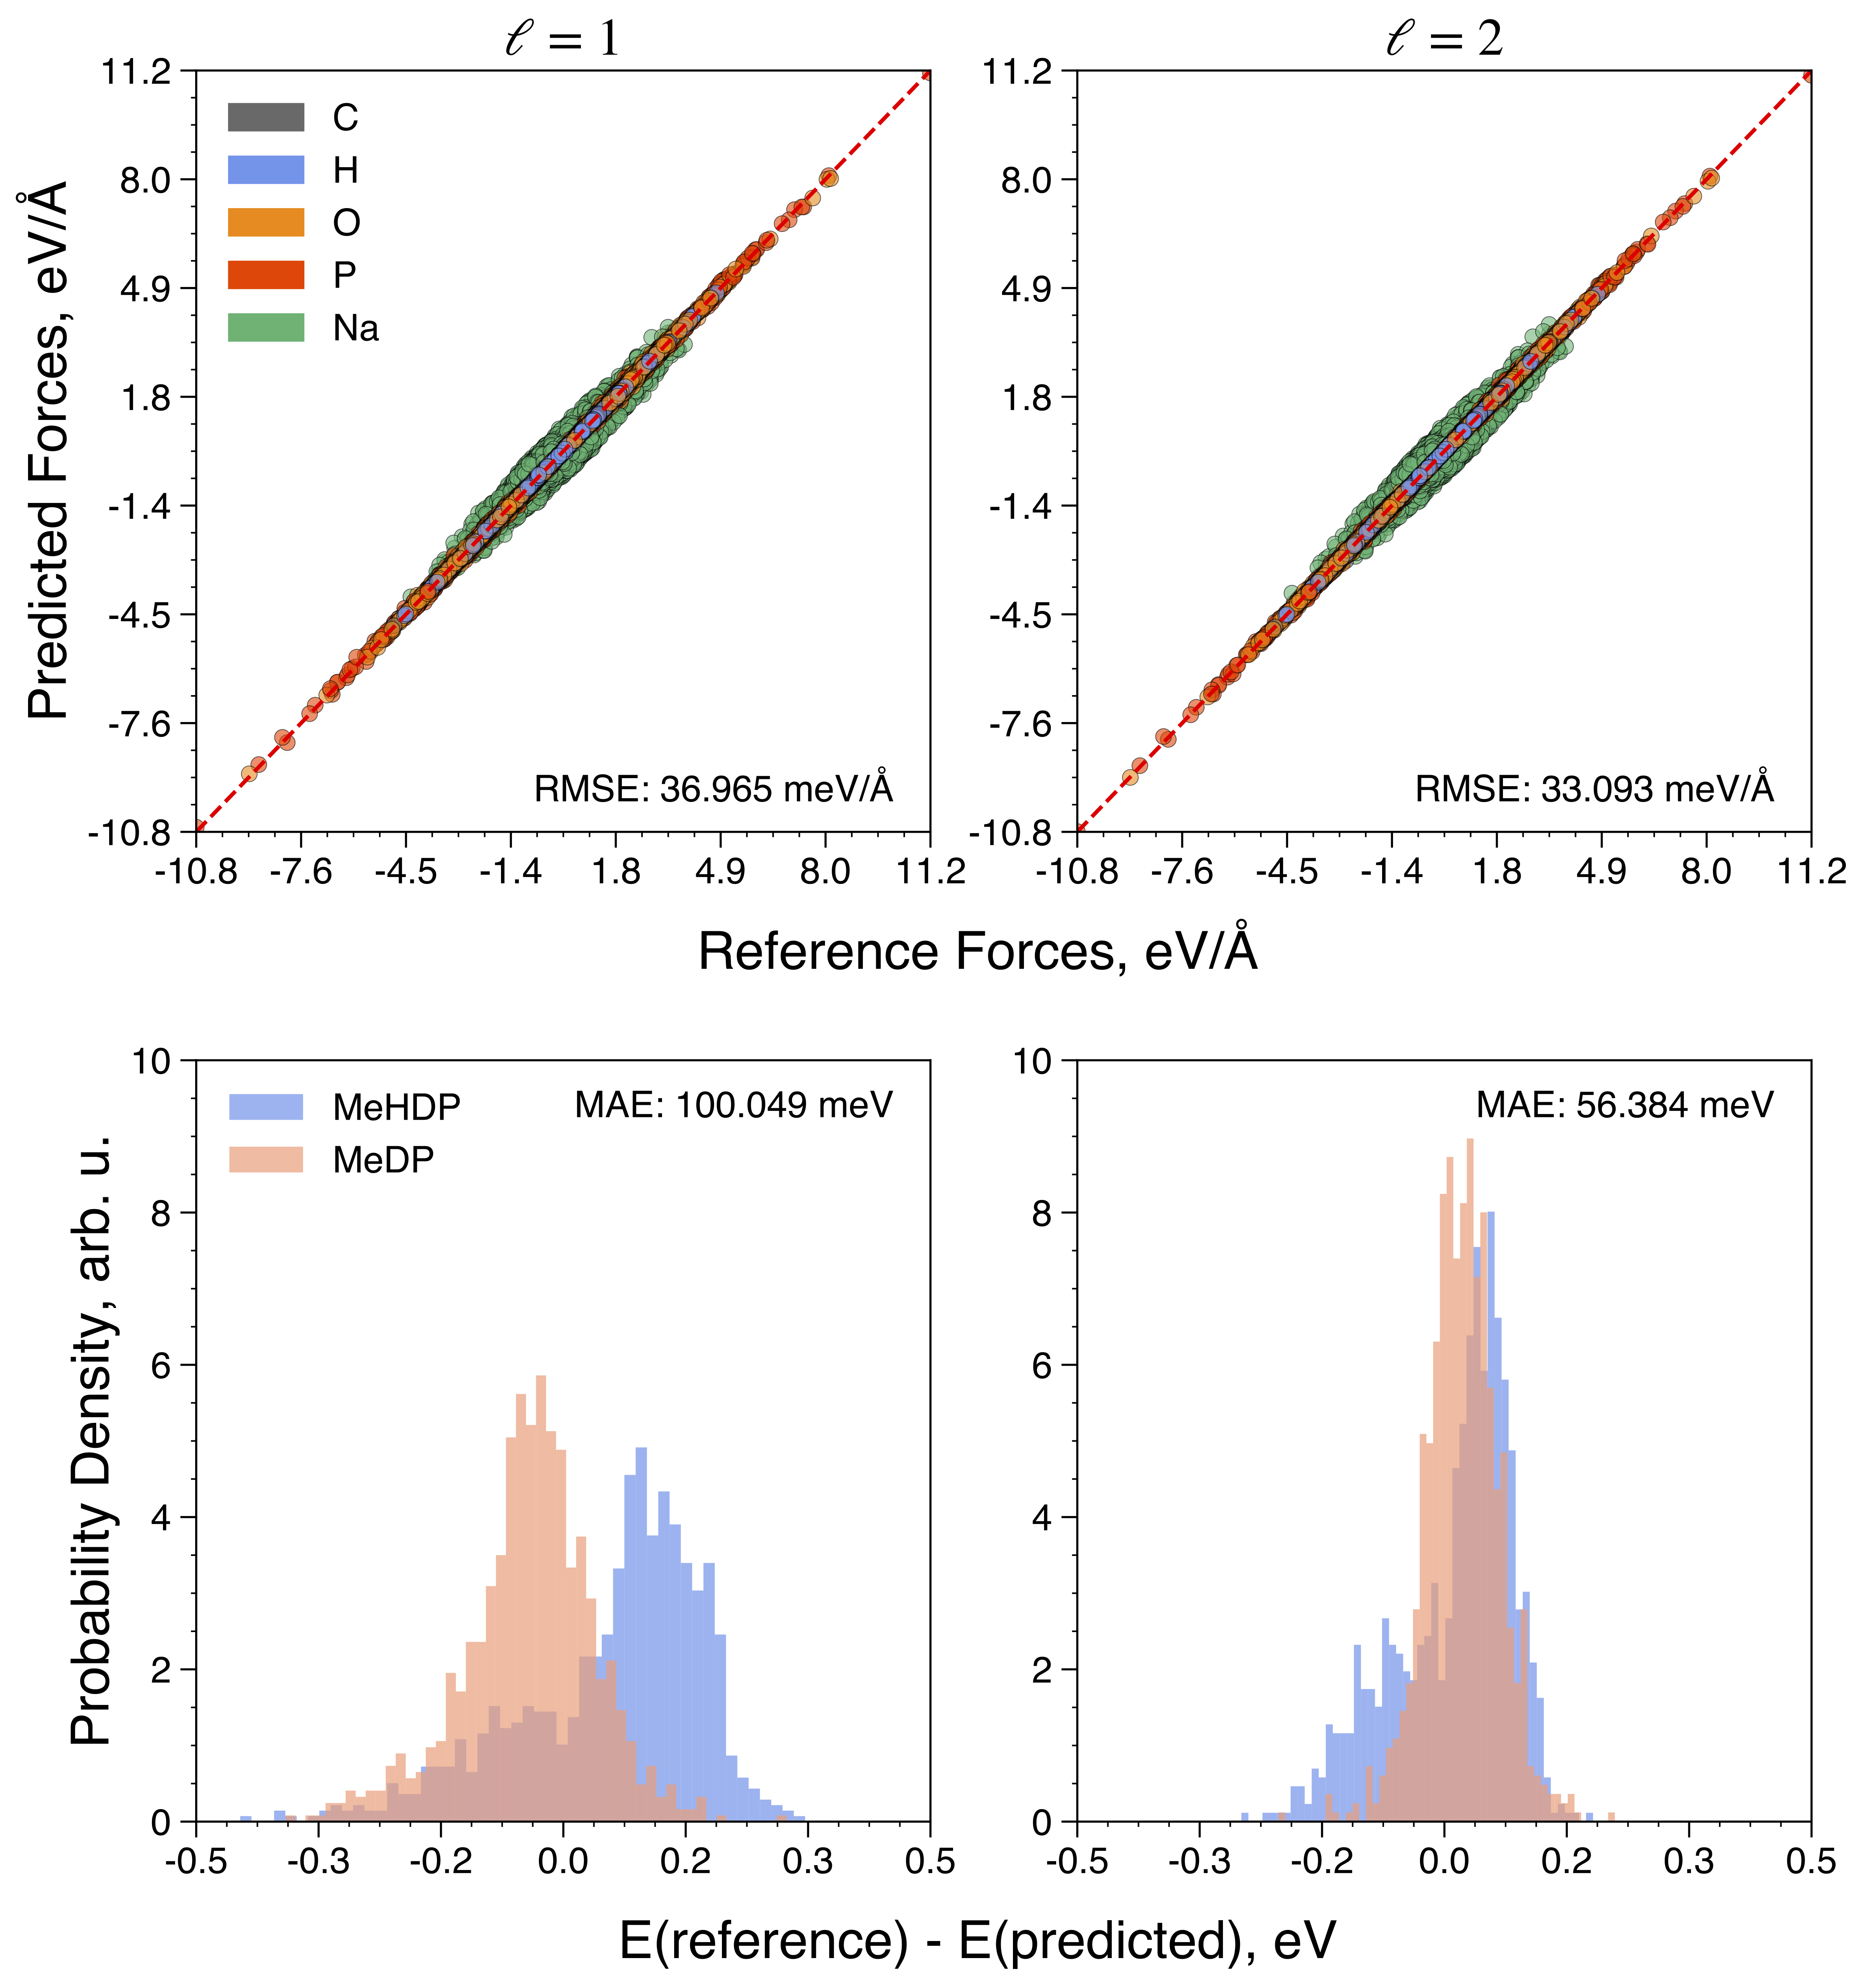
\includegraphics[width=0.8\textwidth]{Figures/4_Results/results_nnp_accuracy_l-1_l-2.png}
    \caption{Accuracy of the neural network potential trained on 12,000 data points. The left panel shows the errors in the forces and energy for the tensor rank $\ell=1$ and the right panel shows the errors for $\ell=2$. The errors are calculated as the difference between the neural network potential and the reference DFT values. For the histograms, the number of bins was set to 50.}
    \label{fig:nnp_accuracy}
\end{figure}

\begin{figure}[ht]
    \centering
    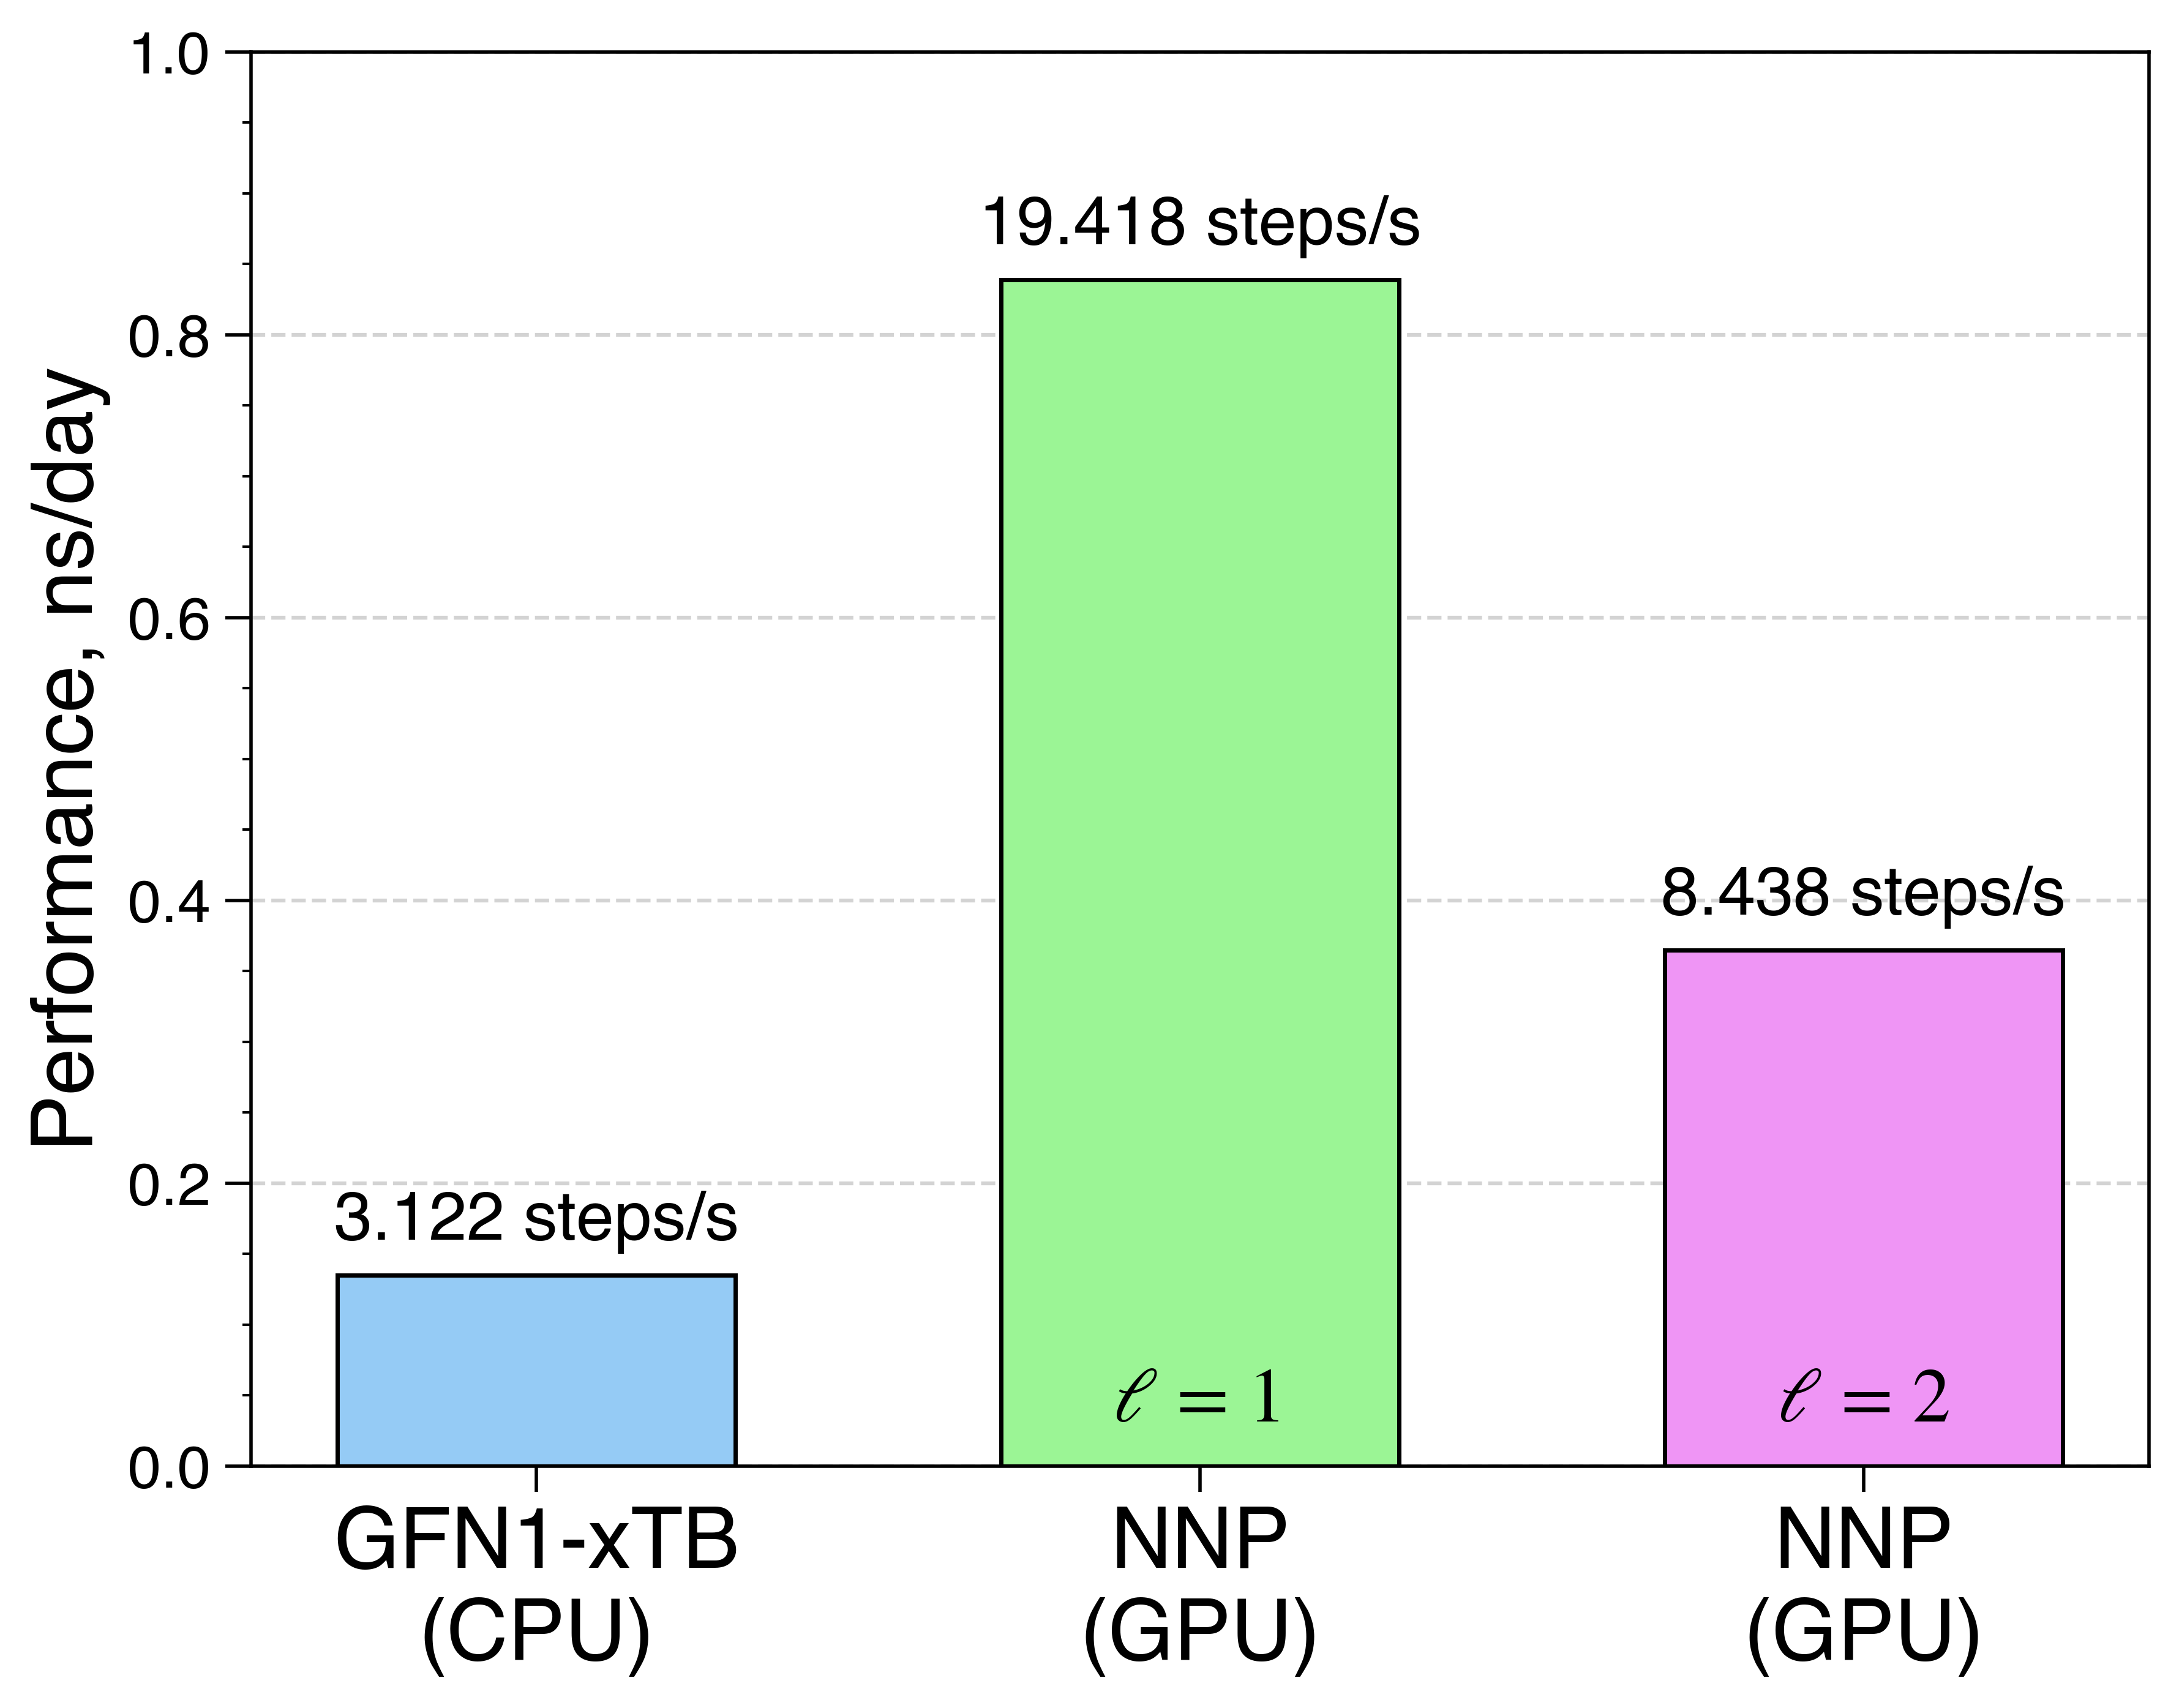
\includegraphics[width=0.6\textwidth]{Figures/4_Results/results_performance_comparison.png}
    \caption{Comparison of the performance between the \textit{ab initio} molecular dynamics runs driven by GFN1-xTB and neural network potentials fitted with the different tensor ranks.}
    \label{fig:performance_comparison}
\end{figure}


%%%%%%%%%%%%%%%%%%%%%%%%%%%%%%%%%%%%%%%%%%%%%%%%%%%%%%%%%%%%%%%%%%%%%%%%%%%%%%%%
\clearpage
\section{Stability of the production runs}



%%%%%%%%%%%%%%%%%%%%%%%%%%%%%%%%%%%%%%%%%%%%%%%%%%%%%%%%%%%%%%%%%%%%%%%%%%%%%%%%
\clearpage
\section{Radial distribution function of water}

\begin{figure}[ht]
    \centering
    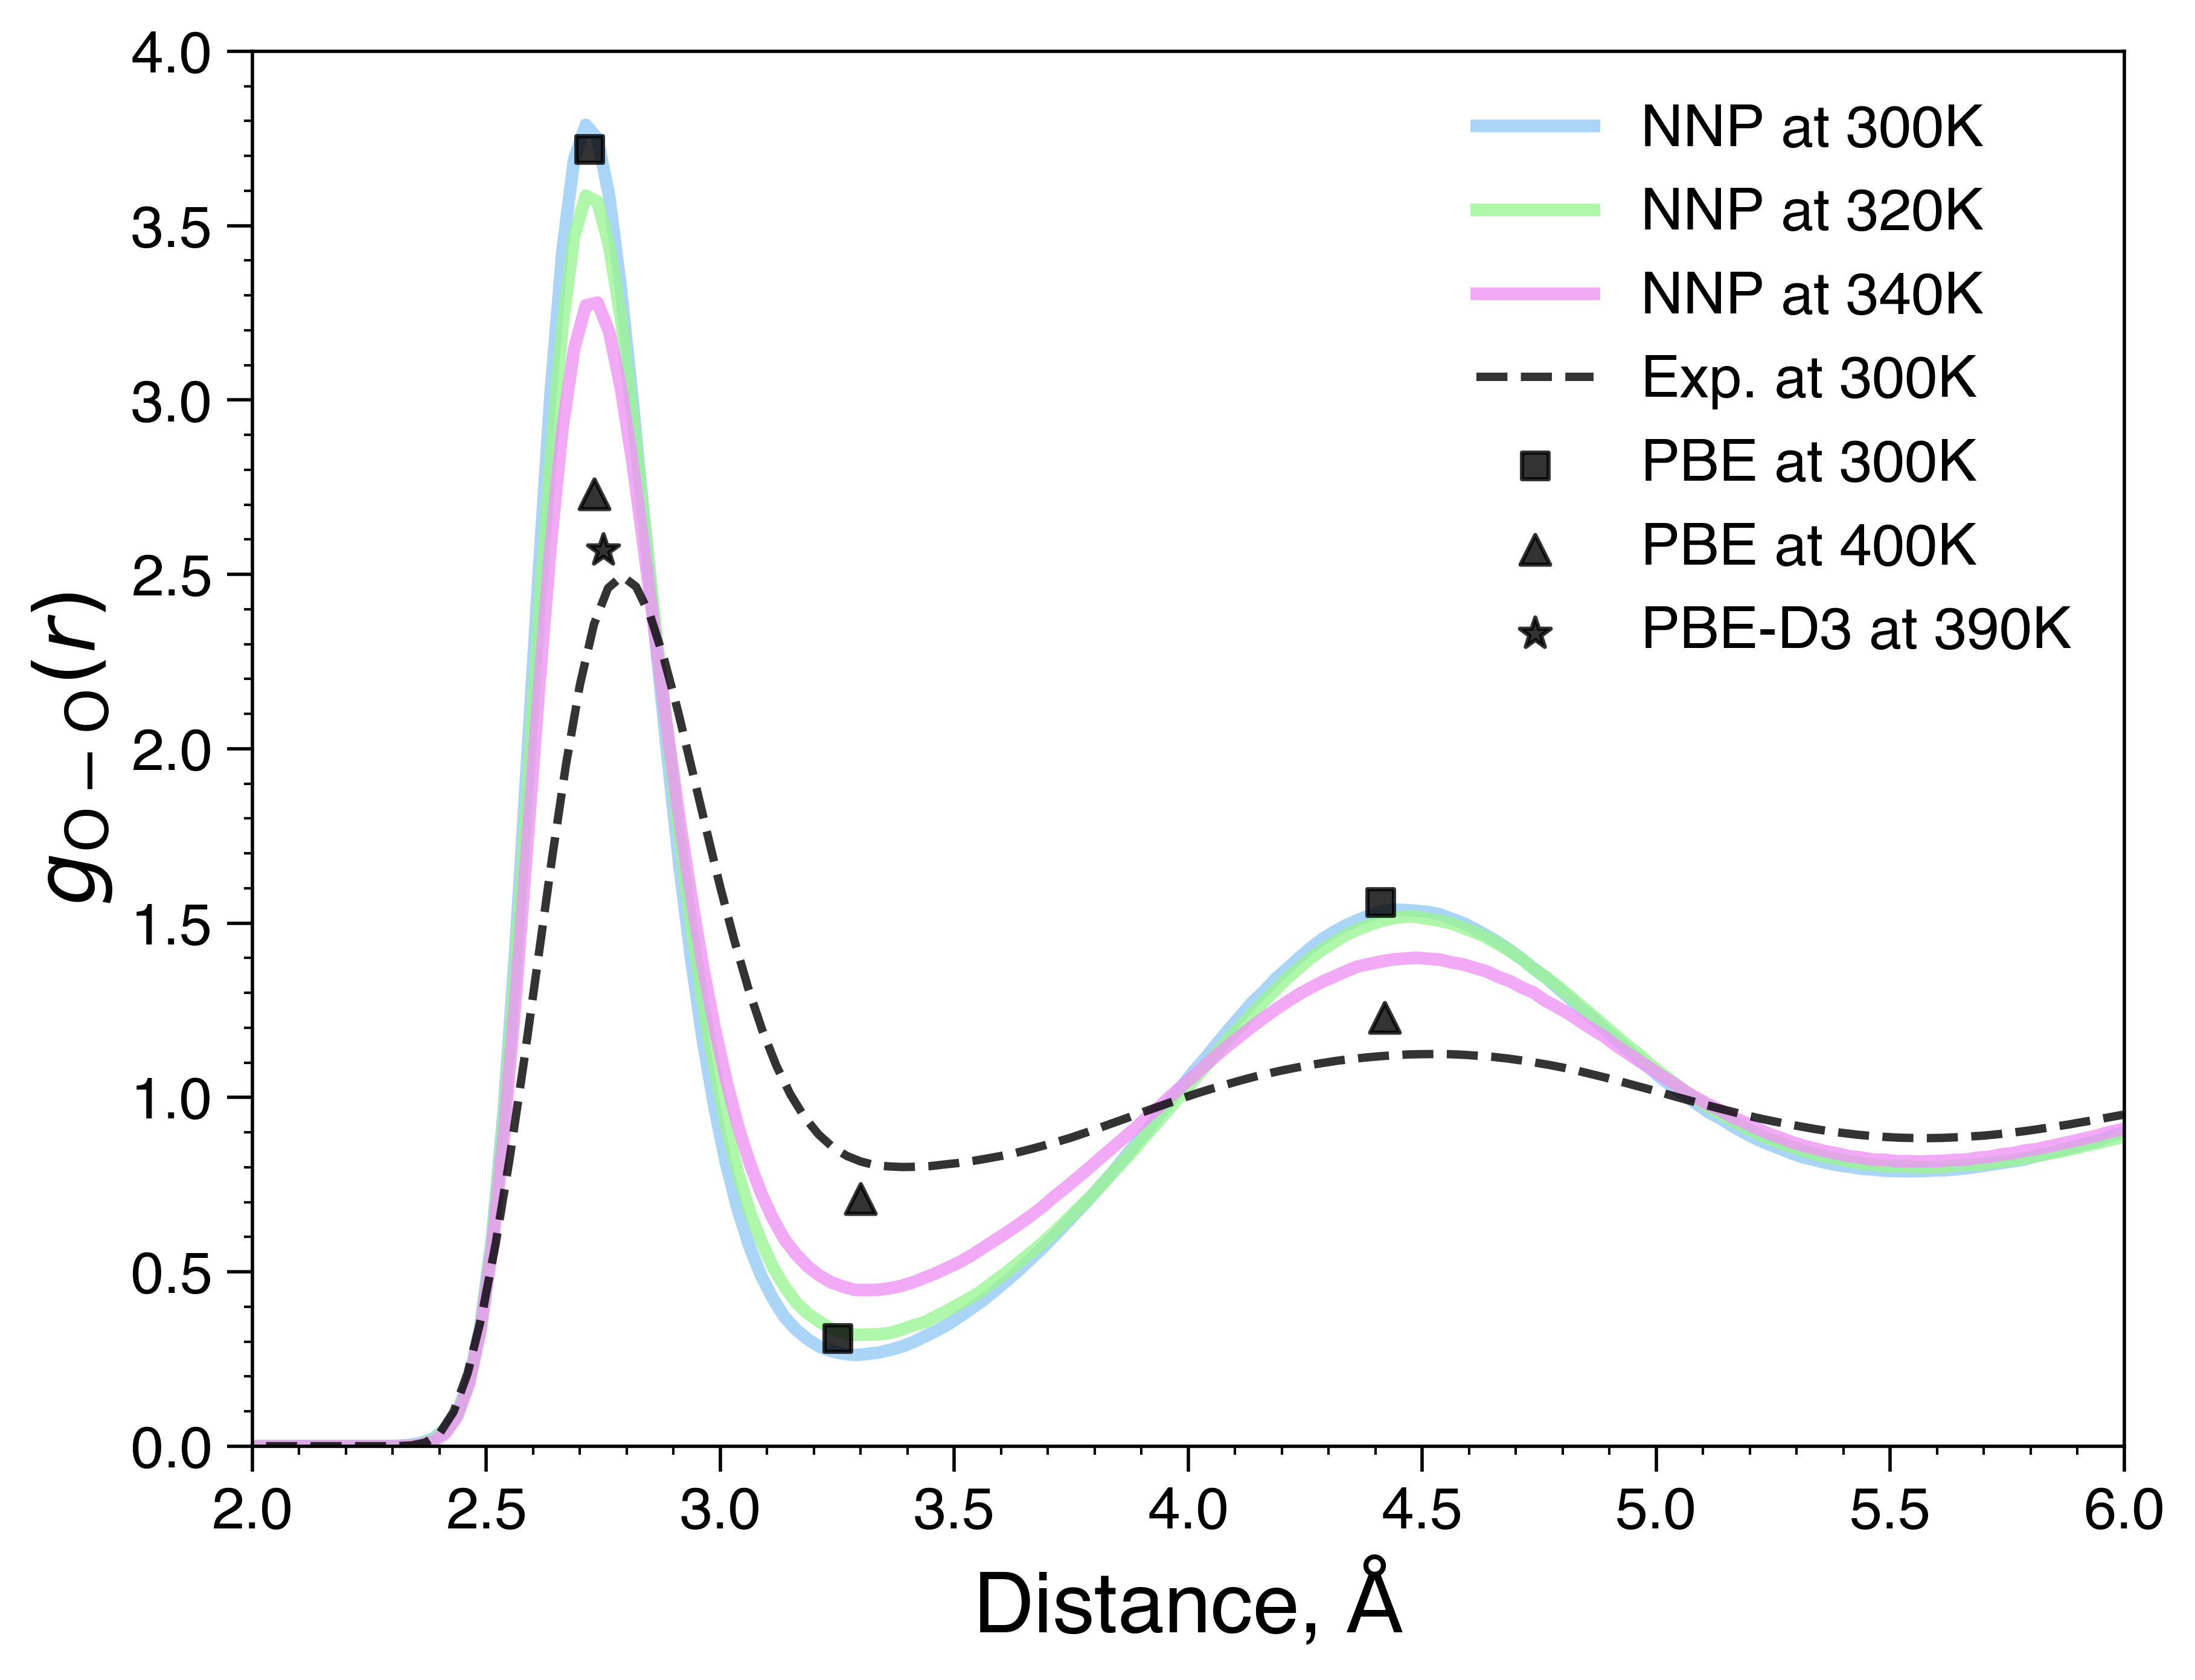
\includegraphics[width=0.6\textwidth]{Figures/4_Results/results_water_rdf.png}
    \caption{\ac{rdf} of water calculated from the production runs at 300, 320, and 340 K. The \acp{rdf} were calculated using the last 2 ns. Experimental data were taken from~\citep{soperRadialDistributionFunctions2013}. The PBE and PBE-D3 were taken from \citep{phamStructureDynamicsAqueous2016} and \citep{zhouQuantifyingStructureWater2022}, respectively.}
    \label{fig:water_rdf}
\end{figure}

%%%%%%%%%%%%%%%%%%%%%%%%%%%%%%%%%%%%%%%%%%%%%%%%%%%%%%%%%%%%%%%%%%%%%%%%%%%%%%%%

\section{Convergence of the free energy profiles}



%%%%%%%%%%%%%%%%%%%%%%%%%%%%%%%%%%%%%%%%%%%%%%%%%%%%%%%%%%%%%%%%%%%%%%%%%%%%%%%%

\section{Evolution of the collective variables over time}



%%%%%%%%%%%%%%%%%%%%%%%%%%%%%%%%%%%%%%%%%%%%%%%%%%%%%%%%%%%%%%%%%%%%%%%%%%%%%%%%


\section{Reaction mechanism for methyl diphosphate trianion}
\subsection{Minimum free energy path and free energy surface}
\subsection{Proton transfer mechanism}



%%%%%%%%%%%%%%%%%%%%%%%%%%%%%%%%%%%%%%%%%%%%%%%%%%%%%%%%%%%%%%%%%%%%%%%%%%%%%%%%

\section{Reaction mechanism for methyl diphosphate dianion}
\subsection{Minimum free energy path and free energy surface}
\subsection{Proton transfer mechanism}



%%%%%%%%%%%%%%%%%%%%%%%%%%%%%%%%%%%%%%%%%%%%%%%%%%%%%%%%%%%%%%%%%%%%%%%%%%%%%%%%

\section{Arrhenius relationship}



%%%%%%%%%%%%%%%%%%%%%%%%%%%%%%%%%%%%%%%%%%%%%%%%%%%%%%%%%%%%%%%%%%%%%%%%%%%%%%%%


\chapter{Conclusions and outlook}

\subsubsection{Final thoughts}
This thesis aimed to investigate the hydrolysis mechanism of methyl diphosphate in water, with a particular focus on the influence of protonation state and solvent environment, by leveraging state-of-the-art neural network potentials and enhanced sampling techniques. The work demonstrates that, by combining data-efficient equivariant graph neural networks (specifically, NequIP) with well-tempered metadynamics, it is possible to obtain detailed free energy surfaces and mechanistic insights for complex, reactive systems at a fraction of the computational cost of traditional \textit{ab initio} molecular dynamics (AIMD).

A comprehensive and diverse dataset was constructed through an iterative learning loop, employing density-aware sampling to ensure balanced coverage of the relevant collective variable space. The final dataset, comprising 12,000 training/validation and 1,800 test configurations, enabled the training of highly accurate \acp{nnp}. The best-performing model, with tensor rank $\ell=1$, achieved force root-mean-square errors (RMSE) of 37 meV/\AA\ and energy mean absolute errors (MAE) below 0.3 meV/atom on the test set - well within the range considered a very good fit by current community standards. Notably, this level of accuracy was achieved with a relatively modest dataset size, highlighting the data efficiency of equivariant GNNs.

The NNP-driven AIMD simulations showed excellent stability over nanosecond \; timescales, with no evidence of numerical instabilities or unphysical artefacts. The structural properties of water, as assessed by the oxygen-oxygen radial distribution function (RDF), were in qualitative agreement with experimental data and previous computational studies at the same level of theory, albeit with some over-structuring typical for the PBE-D3 level of theory at ambient temperature.

For the first time, the nanosecond long sampling of the reaction space was performed which sets ground for the accurate and detailed description of the free energy landscape. The free energy surfaces obtained for both methyl diphosphate trianion (MeDP) and dianion (MeHDP) revealed the presence of both associative and dissociative reaction pathways. For MeDP, the dissociative/concerted (D\textsubscript{N}A\textsubscript{N}) pathway was found to be energetically preferred, with a barrier height of 28.22~kcal/mol, in excellent agreement with the experimental value of 29.2~kcal/mol. The associative pathway was also accessible but featured a significantly higher barrier. In contrast, for MeHDP, the associative/concerted (A\textsubscript{N}D\textsubscript{N}) pathway was better sampled and displayed a lower barrier (30.43~kcal/mol) than the corresponding pathway in MeDP, consistent with the known effect of protonation in enhancing reactivity. The dissociative pathway for MeHDP appeared undersampled, suggesting the need for longer simulations to fully resolve its role.

The analysis of the CV evolution and the observation of multiple recrossings between reactant and product states provided further evidence for the quality of sampling and the reliability of the obtained FES, although full convergence, especially in the transition state regions, remains a challenge. The proton transfer (PT) mechanism was found to involve both 1 and 3 water-mediated pathways, with spontaneous PT events observed during the dynamics, underscoring the ability of the NNP to capture these extremely fast occuring events.

Despite these successes, several caveats must be acknowledged. The accuracy of the NNP is ultimately limited by the quality of the underlying reference data (PBE-D3(BJ)/TZV2P), which is known to over-structure water and may underestimate or overestimate certain reaction barriers. The FES, while showing clear signs of convergence, is not fully converged in the transition state and product regions, particularly for MeHDP. Furthermore, the absence of explicit validation of transition state structures (e.g., via normal mode analysis) means that the precise character of the saddle points remains to be confirmed.

\subsubsection{Future directions}
The results presented in this thesis open several avenues for future research and methodological improvement.

\begin{itemize}
    \item[--] \textit{Extended sampling and FES convergence:} Achieving fully converged free energy surfaces will require longer metadynamics simulations (potentially more than 6 ns, as seen in related studies). Employing multiple-walker metadynamics could accelerate convergence.
    
    \item[--] \textit{Higher-level reference data:} The accuracy of the NNP could be further improved by retraining on reference data generated at a higher level of theory (e.g., hybrid functionals).
    
    \item[--] \textit{Transition state validation:} To unambiguously characterise the nature of the transition states, normal mode analysis should be performed on candidate structures extracted from the FES, confirming the presence of a single imaginary frequency.
      
    \item[--] \textit{Effect of enthalpy and entropy:} In order to see how the enthalpy and entropy contribute to the overall reaction barrier, it would be advantageous to perform biased simulations at different temperatures and get by means of linear fit the enthalpic and entropic contributions from the $\Delta G^{\ddagger} = \Delta H^{\ddagger} - T \Delta S^{\ddagger}$ relation. This would provide a more complete picture of the reaction mechanism.
   
    \item[--] \textit{Explicit treatment of \ac{pt}:} The spontaneous \ac{pt} events observed here suggest that the NNP is capable of capturing proton dynamics, but a more systematic investigation, potentially using dedicated CVs for PT and enhanced sampling along these coordinates, would provide deeper insight into the PT mechanism.
    
    \item[--] \textit{Extension to more complex systems:} The workflow developed here can be readily extended to study the hydrolysis of more complex phosphate esters (e.g., ADP, ATP, GTP) and to include the effects of metal ions (such as Mg$^{2+}$). Such studies would bridge the gap between model systems and biological reality.
\end{itemize}

In summary, this thesis demonstrates the feasibility and power of combining machine learning interatomic potentials with enhanced sampling to unravel complex reaction mechanisms in solution. While challenges remain, particularly in achieving full FES convergence and in addressing the limitations of the underlying electronic structure methods, the approach outlined here provides a practical and scalable framework for future studies of chemical reactivity in realistic environments. As neural network potentials continue to improve, they are likely to become an indispensable tool in the computational chemist's toolkit, enabling the exploration of chemical space with unprecedented accuracy and efficiency.

\bibliographystyle{naturemag}
\phantomsection
\addcontentsline{toc}{chapter}{Bibliography}
\bibliography{References/references.bib}


\appendix
\chapter{Supplementary information}

\begin{figure}[htbp]
    \centering
    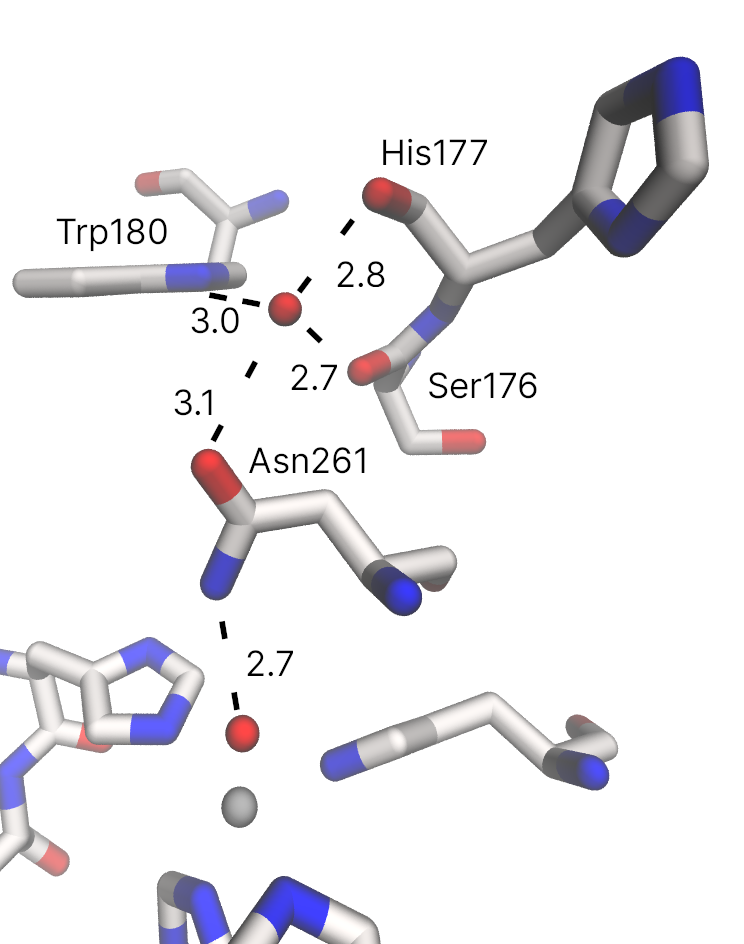
\includegraphics[width=0.5\textwidth]{Figures/crystal_water.png}
    \caption{Hydrogen bond network around the conserved Asn261 residue in the crystal structure of mouse SCD1 (PDB: 4YMK, \cite{Bai2015}). Based on the network, the other Asn rotamer should be more favorable. Colours: silver, zinc; red, oxygen; blue, nitrogen; white, carbon.}
    \label{fig:Crystal_water}
\end{figure}

\begin{table}[htbp]
\centering
\caption{Reactivity of rat stearoyl-CoA desaturase with different acyl-CoA substrates. $K_{m}$ and the Relative maximal velocity are determined by Lineweaver-Burk plots. Some $K_{m}$ values are not measured due to low activity. Adapted from \cite{Enoch1976}.}
\scalebox{0.8}{\begin{tabular}{@{}lcc@{}}
\toprule
\multicolumn{1}{c}{Compound tested} & $K_m$      & \begin{tabular}[c]{@{}c@{}}Relative\\ maximal\\ velocity\end{tabular} \\ \midrule
                                    & $\mu M$    & \%                                                                    \\
Decanoyl-CoA                        & -          & \textless 1                                                           \\
Dodecanoyl-CoA                      & -          & 7                                                                     \\
Tridecanoyl-CoA                     & 8.0        & 50                                                                    \\
Tetradecanoyl-CoA                   & 4.7        & 69                                                                    \\
Hexadecanoyl-CoA (palmitoyl-CoA)    & 4.7        & 86                                                                    \\
Heptadecanoyl-CoA                   & 5.0        & 103                                                                   \\
Octadecanoyl-CoA (stearoyl-CoA)     & 4.5        & 100                                                                   \\
Nonadecanoyl-CoA                    & 5.0        & 103                                                                   \\
Eicosanoyl-CoA (20:0)               & -          & \textless 1                                                           \\ \bottomrule
\end{tabular}}
\label{tab:Enoch_table}
\end{table}

\begin{figure}[htbp]
    \centering
    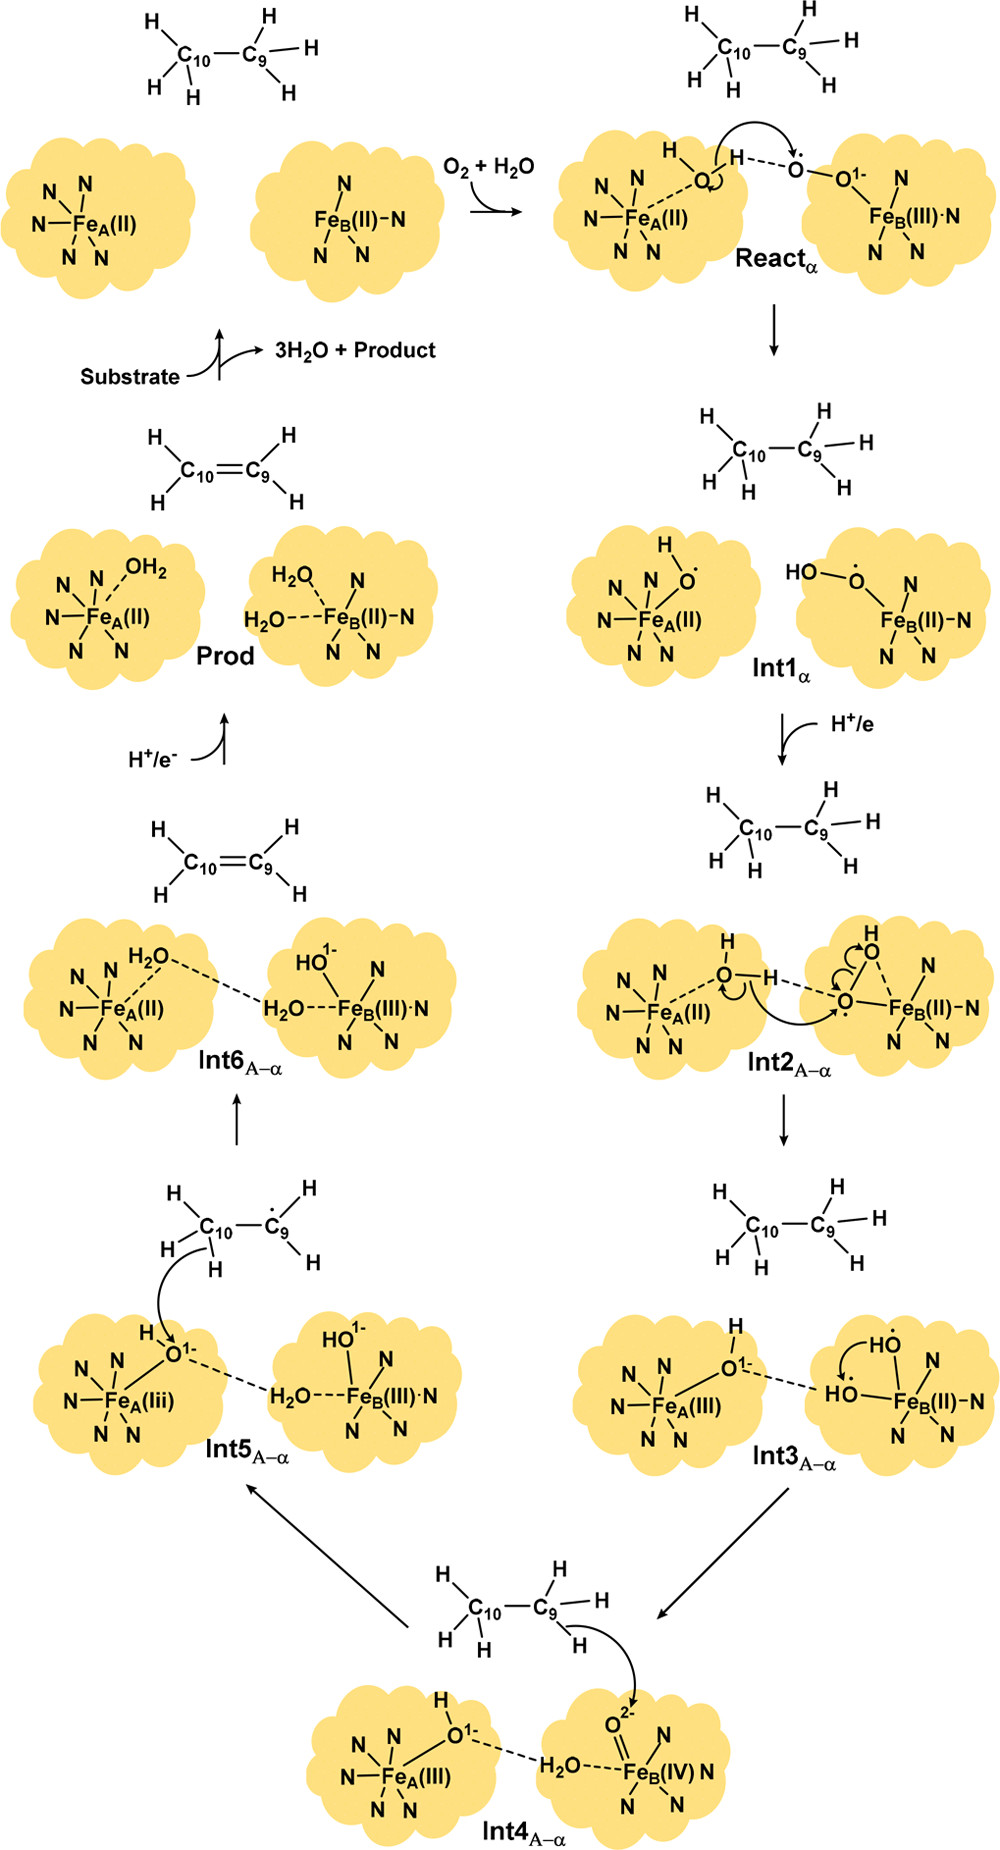
\includegraphics[width=0.65\textwidth]{Figures/Yu_mechanism.jpeg}
    \caption{Proposed reaction mechanism of stearoyl-CoA desaturase based on a cluster model DFT/B3LYP study. Directly taken from \cite{Yu2019}. Note: the exact characterisation of the shown species is not always completely clear. For example, Int3$_{A-\alpha}$ on Fe$_{\text{B}}$ is shown as a dihydroxyl Fe$_{\text{B}}$(II)$-$($\cdot$OH)$_2$ radical but it also has dihydroxo Fe$_{\text{B}}$(IV)$-$(OH)$_{2}^{2-}$ character, so the process from Int3$_{A-\alpha}$ to Int4$_{A-\alpha}$ can be described either as an internal proton transfer or hydrogen atom transfer. In this thesis Int4$_{A-\alpha}$ is referred to as intermediate A.}
    \label{fig:SCD1_mechanism}
\end{figure}


\begin{table}[htbp]
\caption{Equilibration protocol used for classical molecular dynamics simulations of SCD1.}
\centering
\scalebox{0.8}{\begin{tabular}{@{}ccccccc@{}}
\toprule
Run & Calculation type        & Restraints {[}kcal/mol $^2${]}                                                           & Constant & \begin{tabular}[c]{@{}c@{}}Minimization steps / \\ simulation time\end{tabular} & Shake & Timestep {[}fs{]} \\ \midrule
1   & minimization (CPU)      & \begin{tabular}[c]{@{}c@{}}whole protein (100)\\ ST9 (100)\\ membrane (100)\end{tabular} & V        & 1000 steps                                                                      & No    & -                 \\ \midrule
2   & minimization (GPU)      & \begin{tabular}[c]{@{}c@{}}whole protein (100)\\ ST9 (100)\\ membrane (100)\end{tabular} & V        & 10 000 steps                                                                    & No    & -                 \\ \midrule
3   & minimization (CPU)      & \begin{tabular}[c]{@{}c@{}}whole protein (100)\\ ST9 (100)\end{tabular}                  & V        & 1000 steps                                                                      & No    & -                 \\ \midrule
4   & minimization (GPU)      & \begin{tabular}[c]{@{}c@{}}whole protein (100)\\ ST9 (100)\end{tabular}                  & V        & 10 000 steps                                                                    & No    & -                 \\ \midrule
5   & minimization (CPU)      & -                                                                                        & V        & 10 000 steps                                                                    & No    & -                 \\ \midrule
6   & heating (CPU) 0-100 K   & \begin{tabular}[c]{@{}c@{}}whole protein (5)\\ ST9 (5)\\ membrane (5)\end{tabular}       & V        & 5 ps                                                                            & Yes   & 1                 \\ \midrule
7   & heating (GPU) 100-300 K & \begin{tabular}[c]{@{}c@{}}whole protein (5)\\ ST9 (5)\\ membrane (5)\end{tabular}       & P        & 100 ps                                                                          & Yes   & 1                 \\ \midrule
8   & equilibration (GPU)     & \begin{tabular}[c]{@{}c@{}}whole protein (5)\\ ST9 (5)\end{tabular}                      & P        & 1 ns                                                                            & Yes   & 1                 \\ \midrule
9   & equilibration (GPU)     & \begin{tabular}[c]{@{}c@{}}backbone (5)\\ ST9 (5)\end{tabular}                           & P        & 1 ns                                                                            & Yes   & 1                 \\ \midrule
10  & equilibration (GPU)     & \begin{tabular}[c]{@{}c@{}}alpha carbons (5)\\ ST9 (5)\end{tabular}                      & P        & 1 ns                                                                            & Yes   & 1                 \\ \midrule
11  & equilibration (GPU)     & -                                                                                        & P        & 1 ns                                                                            & Yes   & 1                 \\ \midrule
12  & equilibration (GPU)     & -                                                                                        & P        & 5 ns                                                                            & Yes   & 2                 \\ \bottomrule
\end{tabular}}
\label{tab:eq_protocol}
\end{table}

\begin{figure}[htbp]
    \centering
    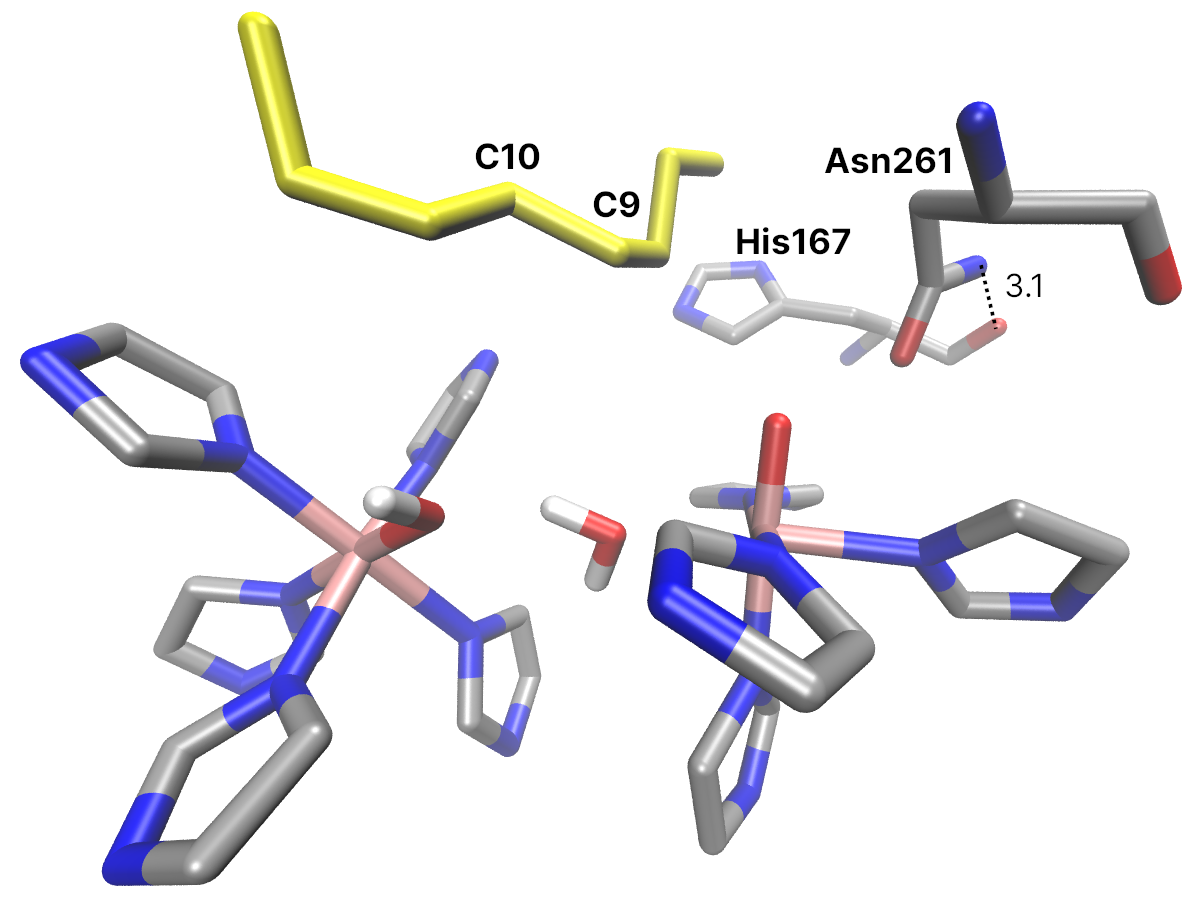
\includegraphics[width=0.8\textwidth]{Figures/int_A_run2.png}
    \caption{Structure of the active site during the second MD production run of intermediate A. Residues are shown as sticks. Distances are shown in Å. Colours: silver, protein carbons; red, oxygen; blue, nitrogen; white, hydrogen; yellow, carbons of stearoyl-CoA; pink, iron. Hydrogen atoms are left out for clarity.}
    \label{fig:intA_run2}
\end{figure}

\begin{figure}[htbp]
    \centering
    \begin{subfigure}{.49\textwidth}
        \centering
        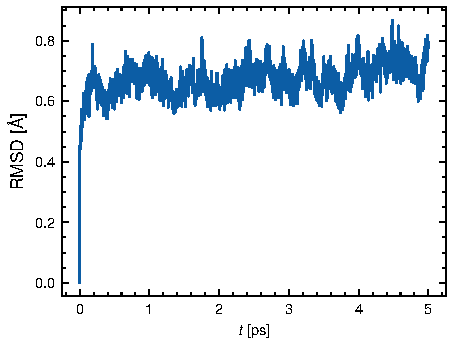
\includegraphics[width=\textwidth]{Figures/B_rmsd.pdf}
    \end{subfigure}
    \begin{subfigure}{.49\textwidth}
        \centering
        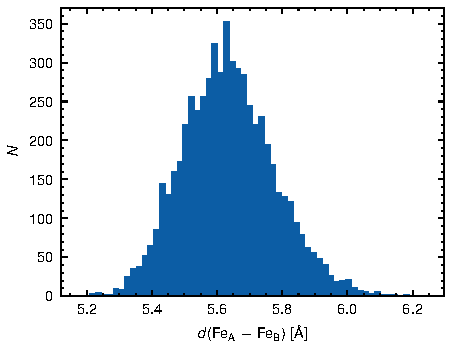
\includegraphics[width=\textwidth]{Figures/B_fe-fe_hist.pdf}
    \end{subfigure}
    \par\bigskip
    \begin{subfigure}{.49\textwidth}
        \centering
        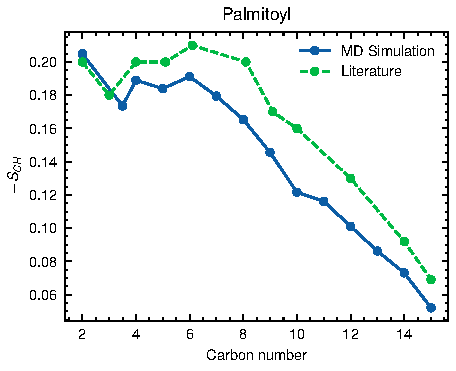
\includegraphics[width=\textwidth]{Figures/B_palmitoyl.pdf}
    \end{subfigure}
    \begin{subfigure}{.49\textwidth}
        \centering
        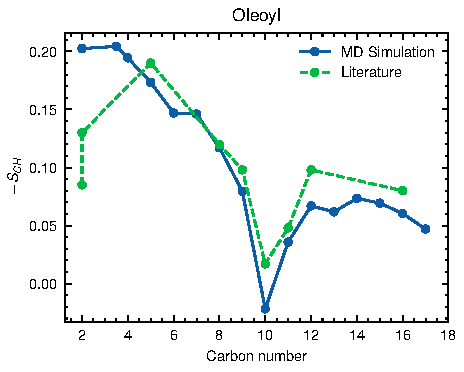
\includegraphics[width=\textwidth]{Figures/B_oleoyl.pdf}
    \end{subfigure}
    \caption{Data to assess the equilibration of intermediate B taken from the last 5 ns equilibration run. RMSD of the protein's backbone alpha carbon atoms with respect to the first frame (top left). Distribution of the iron-iron distance (top right). Average lipid order parameters for the palmitoyl chain of POPC (bottom left). Average lipid order parameters for the oleoyl chain of POPC (bottom right). Experimental values for the lipid order parameters are taken from \cite{Seelig1978,Perly1985}.}
    \label{fig:B_equilibration}
\end{figure}


\begin{figure}[htbp]
    \centering
    \begin{subfigure}{\textwidth}
        \centering
        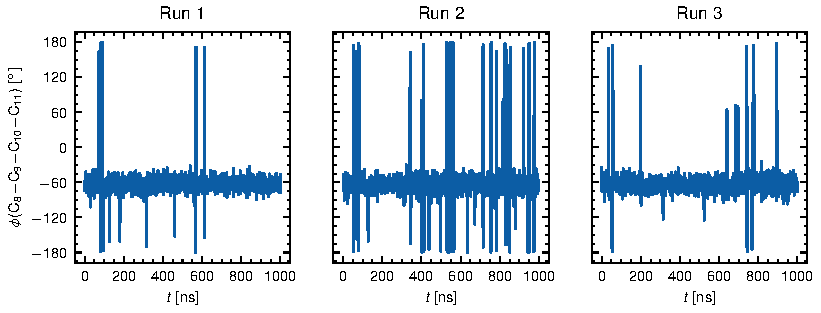
\includegraphics[width=\textwidth]{Figures/B_C9-C10_all.pdf}
    \end{subfigure}
    \par\bigskip
    \begin{subfigure}{\textwidth}
        \centering
        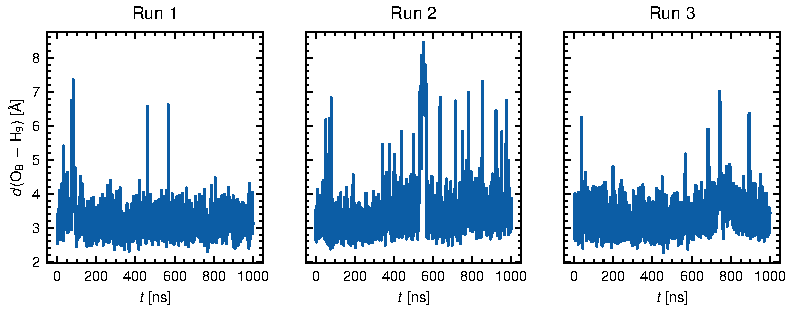
\includegraphics[width=\textwidth]{Figures/B_Ob-H9_all.pdf}
    \end{subfigure}
    \par\bigskip
    \begin{subfigure}{\textwidth}
        \centering
        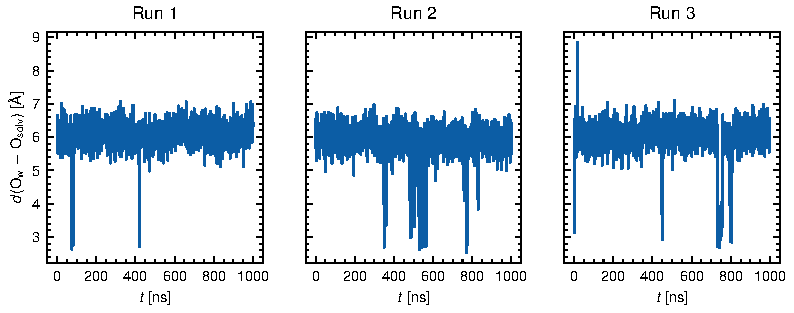
\includegraphics[width=\textwidth]{Figures/B_Ow-Ow_all.pdf}
    \end{subfigure}
    \caption{Data from the three 1 $\mu$s production runs of intermediate B: value of the C$_8-$C$_9-$C$_{10}-$C$_{11}$ dihedral angle of the substrate (top); distance between the oxo oxygen (O$_{\text{B}}$) and \textit{pro}-R hydrogen on C$_9$ (H$_{9}$) that needs to get abstracted (middle); distance between the oxygen of the active site water ligand (O$_{\text{W}}$) and oxygen of a nearby solvent water molecule in the substrate tunnel (bottom). Note: due to the cyclical nature of the dihedral angles the values around 180$^{\circ}$ and $-$180$^{\circ}$ correspond to the same \textit{anti} conformation.}
    \label{fig:B_appendix}
\end{figure}

\begin{figure}
    \centering
    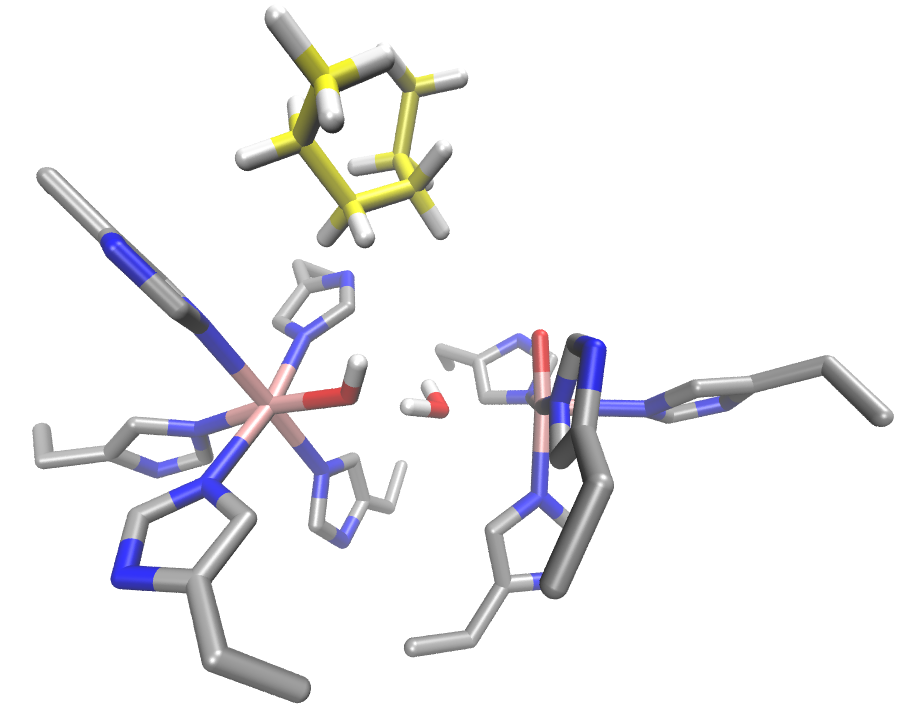
\includegraphics[width=0.7\textwidth]{Figures/intA_xtb.png}
    \caption{Structure of intermediate A after optimization with GFN2-xTB. Residues are shown as sticks. Distances are shown in Å. Colours: silver, protein carbons; red, oxygen; blue, nitrogen; white, hydrogen; yellow, carbons of stearoyl-CoA; pink, iron. Protein's hydrogen atoms are left out for clarity.}
    \label{fig:xtb_intA}
\end{figure}

\begin{figure}
    \centering
    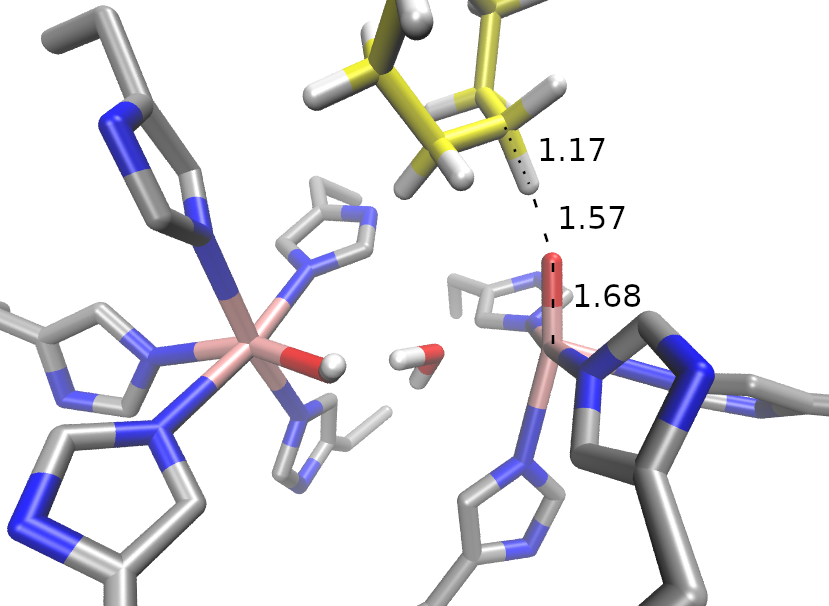
\includegraphics[width=0.7\textwidth]{Figures/TS_xtb.png}
    \caption{Structure of the predicted TS from the GFN2-xTB cluster model PES scan. Residues are shown as sticks. Distances are shown in Å. Colours: silver, protein carbons; red, oxygen; blue, nitrogen; white, hydrogen; yellow, carbons of stearoyl-CoA; pink, iron. Protein's hydrogen atoms are left out for clarity.}
    \label{fig:xtb_TS}
\end{figure}

\begin{table}[htbp]
\caption{Spin densities of the TS predicted by the GFN2-xTB cluster model relaxed potential energy surface scan of intermediate A. Predicted values with B3LYP are taken from \cite{Yu2019}.}
\centering
\begin{tabular}{@{}ccc@{}}
\toprule
\textbf{Atom} & \textbf{\textit{S}$_\text{B3LYP}$} & \textbf{\textit{S}$_\text{GFN2-xTB}$} \\ \midrule
Fe$_{\text{A}}$           & 4.14            & 3.86               \\ \midrule
O$_{\text{A}}$             & 0.27            & 0.25               \\ \midrule
Fe$_{\text{B}}$            & -3.80           & 2.72               \\ \midrule
O$_{\text{B}}$             & -0.25           & 0.64               \\ \midrule
C$_{\text{9}}$             & 0.30            & 0.20               \\ \bottomrule
\end{tabular}
\label{tab:xtb_spin}
\end{table}

\begin{figure}[htbp]
    \centering
    \begin{subfigure}{.49\textwidth}
        \centering
        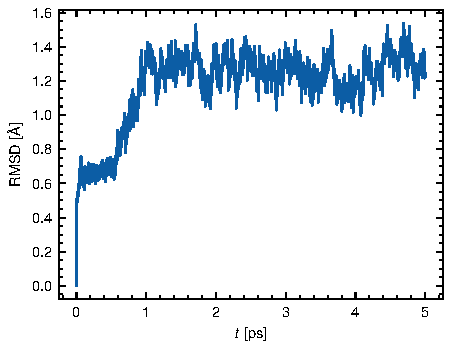
\includegraphics[width=\textwidth]{Figures/TIP3P_rmsd.pdf}
    \end{subfigure}
    \begin{subfigure}{.49\textwidth}
        \centering
        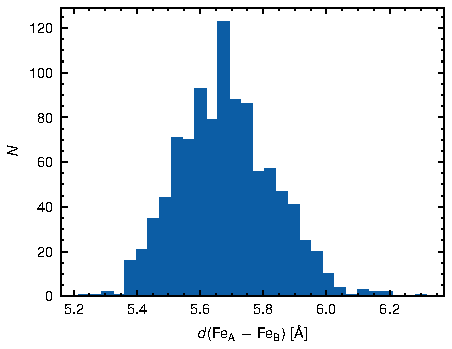
\includegraphics[width=\textwidth]{Figures/TIP3P_fe-fe_hist.pdf}
    \end{subfigure}
    \par\bigskip
    \begin{subfigure}{.49\textwidth}
        \centering
        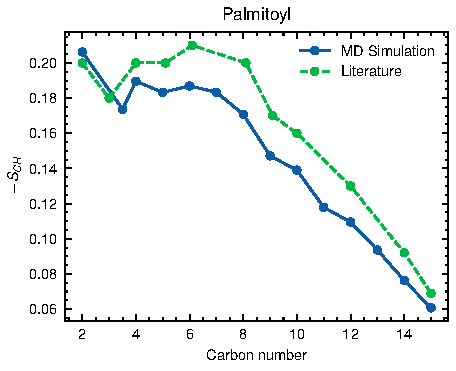
\includegraphics[width=\textwidth]{Figures/TIP3P_palmitoyl.pdf}
    \end{subfigure}
    \begin{subfigure}{.49\textwidth}
        \centering
        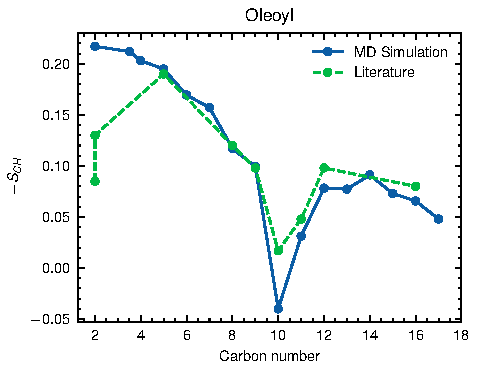
\includegraphics[width=\textwidth]{Figures/TIP3P_oleoyl.pdf}
    \end{subfigure}
    \caption{Data to assess the equilibration of intermediate B with the TIP3P water model taken from the last 5 ns equilibration run. RMSD of the protein's backbone alpha carbon atoms with respect to the first frame (top left). Distribution of the iron-iron distance (top right). Average lipid order parameters for the palmitoyl chain of POPC (bottom left). Average lipid order parameters for the oleoyl chain of POPC (bottom right). Experimental values for the lipid order parameters are taken from \cite{Seelig1978,Perly1985}.}
    \label{fig:TIP3P_equilibration}
\end{figure}

\begin{figure}[htbp]
    \centering
    \begin{subfigure}{\textwidth}
        \centering
        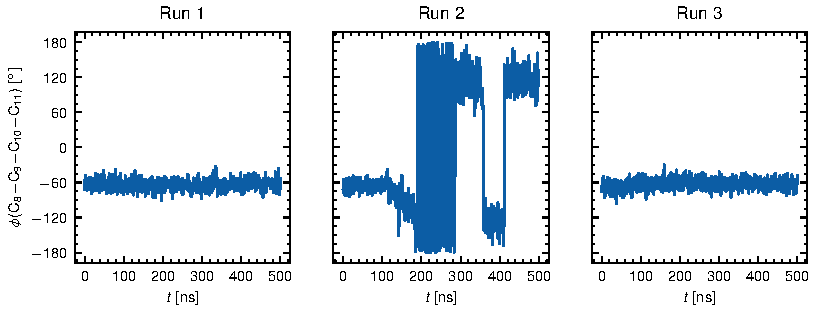
\includegraphics[width=\textwidth]{Figures/xtb_C9-C10_all.pdf}
    \end{subfigure}
    \par\bigskip
    \begin{subfigure}{\textwidth}
        \centering
        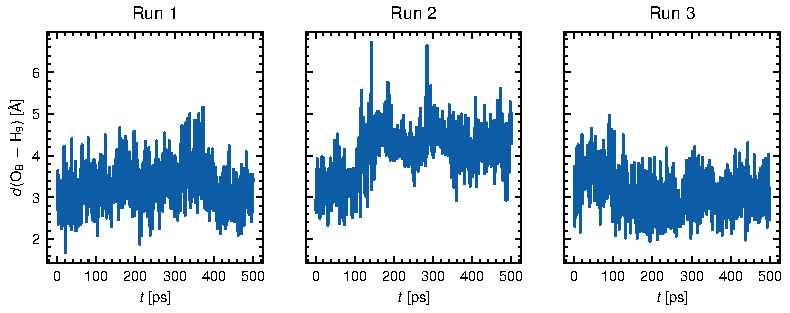
\includegraphics[width=\textwidth]{Figures/xtb_Ob-H9_all.pdf}
    \end{subfigure}
    \par\bigskip
    \begin{subfigure}{\textwidth}
        \centering
        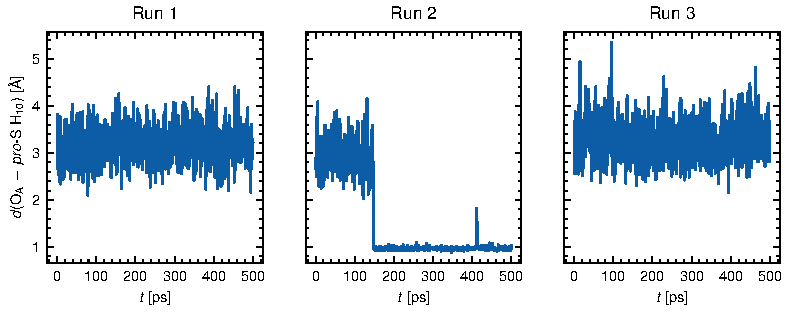
\includegraphics[width=\textwidth]{Figures/xtb_Oa-proSH10_all.pdf}
    \end{subfigure}
    \caption{Data from the three 500 ps QM/MM MD production runs of intermediate B with GFN2-xTB: value of the C$_8-$C$_9-$C$_{10}-$C$_{11}$ dihedral angle of the substrate (top); distance between the oxo oxygen (O$_{\text{B}}$) and \textit{pro}-R hydrogen on C$_9$ (H$_{9}$) that needs to get abstracted (middle); distance between the hydroxide oxygen (O$_{\text{A}}$) and \textit{pro}-S hydrogen on C$_{10}$ (bottom). Note: due to the cyclical nature of the dihedral angles the values around 180$^{\circ}$ and $-$180$^{\circ}$ correspond to the same \textit{anti} conformation.}
    \label{fig:xtb_appendix}
\end{figure}

\begin{figure}[htbp]
    \centering
    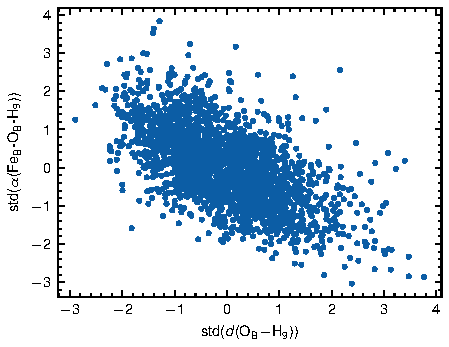
\includegraphics[width=0.6\textwidth]{Figures/2D_plot_starting_frame.pdf}
    \caption{Plot of the standardized values of the Fe$_{\text{B}}-$O$_{\text{B}}-$H$_{\text{9}}$ angle and O$_{\text{B}}-$H$_{\text{9}}$ distance during the first and third QM/MM MD production runs with GFN2-xTB of intermediate B.}
    \label{fig:starting_frame}
\end{figure}

\begin{figure}[htbp]
    \centering
    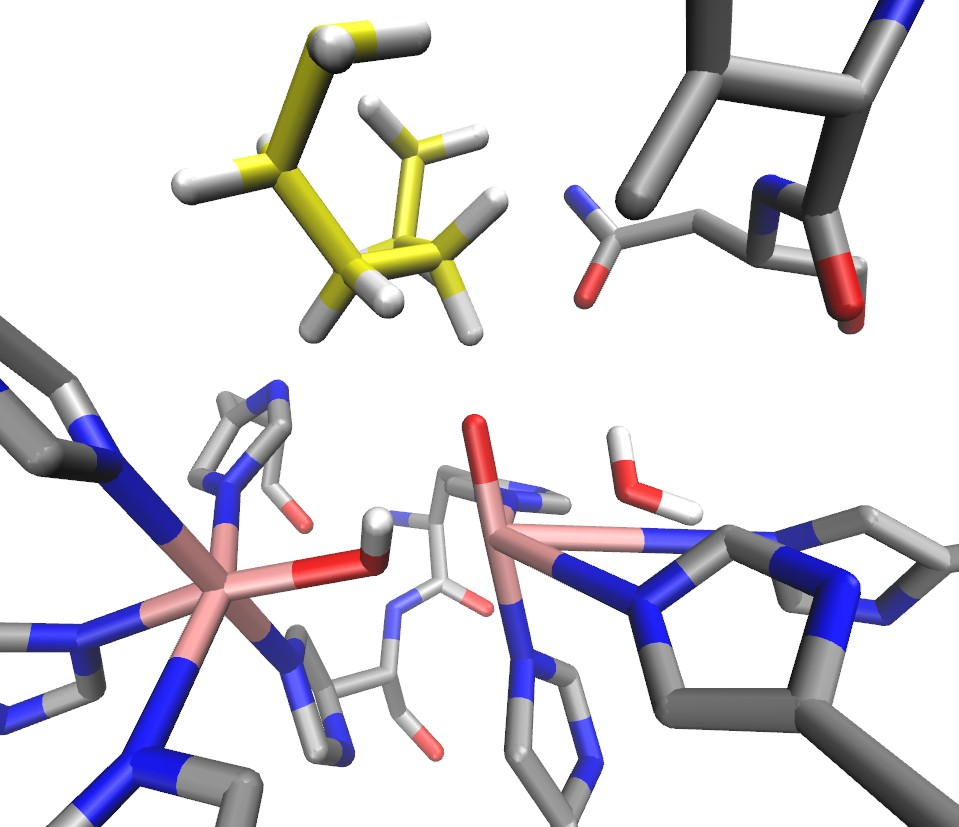
\includegraphics[width=0.7\textwidth]{Figures/pmf_window_28.png}
    \caption{Structure of the system sampled in the $\xi=0.225$ Å umbrella sampling window of intermediate B. Residues are shown as sticks. Distances are shown in Å. Colours: silver, protein carbons; red, oxygen; blue, nitrogen; white, hydrogen; yellow, carbons of stearoyl-CoA; pink, iron. Protein hydrogen atoms are left out for clarity.}
    \label{fig:pmf_window_28}
\end{figure}




\newpage
% ----------------------- Back cover ------------------------------
% Please fill in:
% - Department
% - Department's address
% - Telephone number and fax number
% -----------------------------------------------------------------
\thispagestyle{empty}
\sffamily
%
\begin{textblock}{191}(113,-11)
{\color{blueline}\rule{160pt}{5.5pt}}
\end{textblock}
%
\begin{textblock}{191}(168,-11)
{\color{blueline}\rule{5.5pt}{59pt}}
\end{textblock}
%
\begin{textblock}{183}(-24,-11)
\textblockcolour{}
\flushright
\fontsize{7}{7.5}\selectfont
\textbf{Quantum Chemistry and Physical Chemistry}\\
Celestijnenlaan 200F bus 2404\\
3001 LEUVEN, BELGI\"{E}\\
tel. + 32 16 37 21 98\\
jeremy.harvey@kuleuven.be\\
www.kuleuven.be\\
\end{textblock}
%
\begin{textblock}{191}(154,-7)
\textblockcolour{}
\includegraphics*[height=16.5truemm]{sedes}
\end{textblock}
%
\begin{textblock}{191}(-20,235)
{\color{bluetitle}\rule{544pt}{55pt}}
\end{textblock}
\end{document}
